%%%%%%%%%%%%%%%%%%%%%%%%%%%%%%%%%%%%%%%%%
% Masters/Doctoral Thesis
% LaTeX Template
% Version 2.4 (22/11/16)
%
% This template has been downloaded from:
% http://www.LaTeXTemplates.com
%
% Version 2.x major modifications by:
% Vel (vel@latextemplates.com)
%
% This template is based on a template by:
% Steve Gunn (http://users.ecs.soton.ac.uk/srg/softwaretools/document/templates/)
% Sunil Patel (http://www.sunilpatel.co.uk/thesis-template/)
%
% Template license:
% CC BY-NC-SA 3.0 (http://creativecommons.org/licenses/by-nc-sa/3.0/)
%
%%%%%%%%%%%%%%%%%%%%%%%%%%%%%%%%%%%%%%%%%

%----------------------------------------------------------------------------------------
%	PACKAGES AND OTHER DOCUMENT CONFIGURATIONS
%----------------------------------------------------------------------------------------

\documentclass[
11pt, % The default document font size, options: 10pt, 11pt, 12pt
%oneside, % Two side (alternating margins) for binding by default, uncomment to switch to one side
{english, spanish}, % ngerman for German
singlespacing, % Single line spacing, alternatives: onehalfspacing or doublespacing
%draft, % Uncomment to enable draft mode (no pictures, no links, overfull hboxes indicated)
%nolistspacing, % If the document is onehalfspacing or doublespacing, uncomment this to set spacing in lists to single
%liststotoc, % Uncomment to add the list of figures/tables/etc to the table of contents
%toctotoc, % Uncomment to add the main table of contents to the table of contents
%parskip, % Uncomment to add space between paragraphs
%nohyperref, % Uncomment to not load the hyperref package
headsepline, % Uncomment to get a line under the header
%chapterinoneline, % Uncomment to place the chapter title next to the number on one line
%consistentlayout, % Uncomment to change the layout of the declaration, abstract and acknowledgements pages to match the default layout
]{MastersDoctoralThesis} % The class file specifying the document structure

\usepackage[utf8]{inputenc} % Required for inputting international characters
\usepackage[T1]{fontenc} % Output font encoding for international characters

\usepackage{palatino} % Use the Palatino font by default

\usepackage[backend=bibtex,style=authoryear,natbib=true]{biblatex} % Use the bibtex backend with the authoryear citation style (which resembles APA)

\addbibresource{example.bib} % The filename of the bibliography

\usepackage[autostyle=true]{csquotes} % Required to generate language-dependent quotes in the bibliography

%----------------------------------------------------------------------------------------
%	MARGIN SETTINGS
%----------------------------------------------------------------------------------------

\geometry{
	paper=a4paper, % Change to letterpaper for US letter
	inner=2.5cm, % Inner margin
	outer=3.8cm, % Outer margin
	bindingoffset=.5cm, % Binding offset
	top=1.5cm, % Top margin
	bottom=1.5cm, % Bottom margin
	%showframe, % Uncomment to show how the type block is set on the page
}


%----------------------------------------------------------------------------------------
%	MARCIAL SETTINGS
%----------------------------------------------------------------------------------------


\usepackage{titlesec}

\setlength{\parskip}{1em}
\setcounter{secnumdepth}{4}
\titleformat{\paragraph}
{\normalfont\normalsize\bfseries}{\theparagraph}{1em}{}
\titlespacing*{\paragraph}
{0pt}{3.25ex plus 1ex minus .2ex}{1.5ex plus .2ex}

\usepackage{pdfpages}

%----------------------------------------------------------------------------------------
%	THESIS INFORMATION
%----------------------------------------------------------------------------------------

\thesistitle{Banco de Calibración de Zowi} % Your thesis title, this is used in the title and abstract, print it elsewhere with \ttitle
\supervisor{Juan Manuel \textsc{Enrique}} % Your supervisor's name, this is used in the title page, print it elsewhere with \supname
\examiner{} % Your examiner's name, this is not currently used anywhere in the template, print it elsewhere with \examname
\degree{Ingeniería Industrial} % Your degree name, this is used in the title page and abstract, print it elsewhere with \degreename
\author{Marcial \textsc{Rodríguez}} % Your name, this is used in the title page and abstract, print it elsewhere with \authorname
\addresses{} % Your address, this is not currently used anywhere in the template, print it elsewhere with \addressname

\subject{Investigación y Robótica} % Your subject area, this is not currently used anywhere in the template, print it elsewhere with \subjectname
\keywords{} % Keywords for your thesis, this is not currently used anywhere in the template, print it elsewhere with \keywordnames
\university{\href{http://www.uhu.es}{Universidad de Huelva}} % Your university's name and URL, this is used in the title page and abstract, print it elsewhere with \univname
\department{\href{}{}} % Your department's name and URL, this is used in the title page and abstract, print it elsewhere with \deptname
\group{\href{}{}} % Your research group's name and URL, this is used in the title page, print it elsewhere with \groupname
\faculty{\href{http://www.uhu.es/etsi}{Escuela Técnica Superior de Ingeniería}} % Your faculty's name and URL, this is used in the title page and abstract, print it elsewhere with \facname

\AtBeginDocument{
\hypersetup{pdftitle=\ttitle} % Set the PDF's title to your title
\hypersetup{pdfauthor=\authorname} % Set the PDF's author to your name
\hypersetup{pdfkeywords=\keywordnames} % Set the PDF's keywords to your keywords
}

\begin{document}

\frontmatter % Use roman page numbering style (i, ii, iii, iv...) for the pre-content pages

\pagestyle{plain} % Default to the plain heading style until the thesis style is called for the body content

%----------------------------------------------------------------------------------------
%	TITLE PAGE
%----------------------------------------------------------------------------------------

\begin{titlepage}
\begin{center}

\vspace*{.06\textheight}
{\scshape\LARGE \univname\par}\vspace{0.1cm} % University name
{\scshape\Large \facname\par}\vspace{0.8cm} % University name
\textsc{\Large Proyecto Fin de Carrera}\\[0.2cm] % Thesis type

\HRule \\[0.6cm] % Horizontal line
{\huge \bfseries \ttitle\par}\vspace{0.2cm} % Thesis title
\HRule \\[1.2cm] % Horizontal line

\begin{minipage}[t]{0.4\textwidth}
\begin{flushleft} \large
\emph{Autor:}\\
\href{http://uborzz.es}{\authorname} % Author name - remove the \href bracket to remove the link
\end{flushleft}
\end{minipage}
\begin{minipage}[t]{0.4\textwidth}
\begin{flushright} \large
\emph{Coordinador:} \\
\href{}{\supname} % Supervisor name - remove the \href bracket to remove the link
\end{flushright}
\end{minipage}\\[0.1cm]

\vfill
\large \textit{Proyecto Fin de Carrera \\ para la titulación de \degreename}\\[0.3cm] % University requirement text
\textit{realizado en}\\[0.4cm]
% \groupname\\\deptname\\[2cm] % Research group name and department name
Grupo Robótica Industrial y Automatización\\Extinto Dpto. Innovación y Robótica\\BQ\\[2cm] % Research group name and department name

\vfill

{\large \today}\\[1cm] % Date
%\includegraphics{Logo} % University/department logo - uncomment to place it

\vfill
\end{center}
\end{titlepage}

% %----------------------------------------------------------------------------------------
% %	DECLARATION PAGE
% %----------------------------------------------------------------------------------------
%
% \begin{declaration}
% \addchaptertocentry{\authorshipname} % Add the declaration to the table of contents
% \noindent I, \authorname, declare that this thesis titled, \enquote{\ttitle} and the work presented in it are my own. I confirm that:
%
% \begin{itemize}
% \item This work was done wholly or mainly while in candidature for a research degree at this University.
% \item Where any part of this thesis has previously been submitted for a degree or any other qualification at this University or any other institution, this has been clearly stated.
% \item Where I have consulted the published work of others, this is always clearly attributed.
% \item Where I have quoted from the work of others, the source is always given. With the exception of such quotations, this thesis is entirely my own work.
% \item I have acknowledged all main sources of help.
% \item Where the thesis is based on work done by myself jointly with others, I have made clear exactly what was done by others and what I have contributed myself.\\
% \end{itemize}
%
% \noindent Signed:\\
% \rule[0.5em]{25em}{0.5pt} % This prints a line for the signature
%
% \noindent Date:\\
% \rule[0.5em]{25em}{0.5pt} % This prints a line to write the date
% \end{declaration}
%
%\cleardoublepage
%
% %----------------------------------------------------------------------------------------
% %	QUOTATION PAGE
% %----------------------------------------------------------------------------------------

\vspace*{0.2\textheight}

\noindent\enquote{\itshape Everyday we make it, we'll make it the best we can.}\bigbreak

\hfill Jack Daniel

 %----------------------------------------------------------------------------------------
 %	ABSTRACT PAGE
 %----------------------------------------------------------------------------------------

 \begin{abstract}
 \addchaptertocentry{\abstractname} % Add the abstract to the table of contents
 
El lanzamiento de un nuevo producto en la línea de robótica educativa de BQ necesitó la implicación de gran parte de los departamentos de la empresa. En este momento el autor de este proyecto y miembro del Departamento de Innovación y Robótica, trabajaba en sistemas de automatización y visión por computador.

Este documento recoge la información sobre el diseño de un sistema, basado en Arduino, Raspberry y sensores IMU, que da solución al problema del calibrado automático en línea de producción de los servomotores del nuevo producto antes mencionado, el robot educativo Zowi. 


 \end{abstract}
 %----------------------------------------------------------------------------------------
 %	ACKNOWLEDGEMENTS
 %----------------------------------------------------------------------------------------

 \begin{acknowledgements}
 \addchaptertocentry{\acknowledgementname} % Add the acknowledgements to the table of contents

Este proyecto cierra una etapa de mi formación que ha sido mucho más larga y discontinuada de lo esperado. Aprovecho para agradecer a todas las personas que me han acompañado en este camino, muchas de ellas con más ganas de verme acabar la titulación que yo mismo.

En primer lugar, gracias a Liss por estar siempre a mi lado y ser mi más fiable fuente de conocimiento y sabiduría.

Gracias a mi familia, mis padres no pueden haberme dicho más veces las palabras: ``Chiquillo, acaba ya la carrera''.

Gracias al Departamento de Innovación y Robótica de BQ construido por Obijuan, por la creación de Zowi, por el puesto de trabajo y por tantos conocimientos adquiridos.

Gracias a la Universidad de Huelva, a mi gran compañero y amigo Emilian, y a Juanma, mi coordinador. Parecía que ésto no iba a acabar nunca, ¿verdad?.

Gracias a los Dofitos, porque sí.

Y por último, mencionar a mis compañeros más directos en mi paso por BQ, que se han convertido en auténticos amigos. Los integrantes del Grupo de Robótica Industrial y Materiales: Santi, Jose Emilio, Chema, Raúl y Javi. En este grupo todo lo que se hacía no solamente se hacía bien, sino que se hacía bonito y original, innovar y crear desde cero era una preferencia para todos los miembros del grupo. Todos los días se volvía a casa con un corte o una quemadura nueva, pero también con una sonrisa. Gracias.


 \end{acknowledgements}

%----------------------------------------------------------------------------------------
%	LIST OF CONTENTS/FIGURES/TABLES PAGES
%----------------------------------------------------------------------------------------

\tableofcontents % Prints the main table of contents

\listoffigures % Prints the list of figures

\listoftables % Prints the list of tables

% %----------------------------------------------------------------------------------------
% %	ABBREVIATIONS
% %----------------------------------------------------------------------------------------
%
% \begin{abbreviations}{ll} % Include a list of abbreviations (a table of two columns)
%
% \textbf{LAH} & \textbf{L}ist \textbf{A}bbreviations \textbf{H}ere\\
% \textbf{WSF} & \textbf{W}hat (it) \textbf{S}tands \textbf{F}or\\
%
% \end{abbreviations}

% %----------------------------------------------------------------------------------------
% %	PHYSICAL CONSTANTS/OTHER DEFINITIONS
% %----------------------------------------------------------------------------------------
%
% \begin{constants}{lr@{${}={}$}l} % The list of physical constants is a three column table
%
% % The \SI{}{} command is provided by the siunitx package, see its documentation for instructions on how to use it
%
% Speed of Light & $c_{0}$ & \SI{2.99792458e8}{\meter\per\second} (exact)\\
% %Constant Name & $Symbol$ & $Constant Value$ with units\\
%
% \end{constants}

% %----------------------------------------------------------------------------------------
% %	SYMBOLS
% %----------------------------------------------------------------------------------------
%
% \begin{symbols}{lll} % Include a list of Symbols (a three column table)
%
% $a$ & distance & \si{\meter} \\
% $P$ & power & \si{\watt} (\si{\joule\per\second}) \\
% %Symbol & Name & Unit \\
%
% \addlinespace % Gap to separate the Roman symbols from the Greek
%
% $\omega$ & angular frequency & \si{\radian} \\
%
% \end{symbols}

% %----------------------------------------------------------------------------------------
% %	DEDICATION
% %----------------------------------------------------------------------------------------
%
% \dedicatory{For/Dedicated to/To my\ldots}

%----------------------------------------------------------------------------------------
%	THESIS CONTENT - CHAPTERS
%----------------------------------------------------------------------------------------

\mainmatter % Begin numeric (1,2,3...) page numbering

\pagestyle{thesis} % Return the page headers back to the "thesis" style

% Include the chapters of the thesis as separate files from the Chapters folder
% Uncomment the lines as you write the chapters

% Chapter 1

\chapter{Chapter Title Here} % Main chapter title

\label{Chapter1} % For referencing the chapter elsewhere, use \ref{Chapter1} 

%----------------------------------------------------------------------------------------

% Define some commands to keep the formatting separated from the content 
\newcommand{\keyword}[1]{\textbf{#1}}
\newcommand{\tabhead}[1]{\textbf{#1}}
\newcommand{\code}[1]{\texttt{#1}}
\newcommand{\file}[1]{\texttt{\bfseries#1}}
\newcommand{\option}[1]{\texttt{\itshape#1}}

%----------------------------------------------------------------------------------------

\section{Welcome and Thank You}
Welcome to this \LaTeX{} Thesis Template, a beautiful and easy to use template for writing a thesis using the \LaTeX{} typesetting system.

If you are writing a thesis (or will be in the future) and its subject is technical or mathematical (though it doesn't have to be), then creating it in \LaTeX{} is highly recommended as a way to make sure you can just get down to the essential writing without having to worry over formatting or wasting time arguing with your word processor.

\LaTeX{} is easily able to professionally typeset documents that run to hundreds or thousands of pages long. With simple mark-up commands, it automatically sets out the table of contents, margins, page headers and footers and keeps the formatting consistent and beautiful. One of its main strengths is the way it can easily typeset mathematics, even \emph{heavy} mathematics. Even if those equations are the most horribly twisted and most difficult mathematical problems that can only be solved on a super-computer, you can at least count on \LaTeX{} to make them look stunning.

%----------------------------------------------------------------------------------------

\section{Learning \LaTeX{}}

\LaTeX{} is not a \textsc{wysiwyg} (What You See is What You Get) program, unlike word processors such as Microsoft Word or Apple's Pages. Instead, a document written for \LaTeX{} is actually a simple, plain text file that contains \emph{no formatting}. You tell \LaTeX{} how you want the formatting in the finished document by writing in simple commands amongst the text, for example, if I want to use \emph{italic text for emphasis}, I write the \verb|\emph{text}| command and put the text I want in italics in between the curly braces. This means that \LaTeX{} is a \enquote{mark-up} language, very much like HTML.

\subsection{A (not so short) Introduction to \LaTeX{}}

If you are new to \LaTeX{}, there is a very good eBook -- freely available online as a PDF file -- called, \enquote{The Not So Short Introduction to \LaTeX{}}. The book's title is typically shortened to just \emph{lshort}. You can download the latest version (as it is occasionally updated) from here:
\url{http://www.ctan.org/tex-archive/info/lshort/english/lshort.pdf}

It is also available in several other languages. Find yours from the list on this page: \url{http://www.ctan.org/tex-archive/info/lshort/}

It is recommended to take a little time out to learn how to use \LaTeX{} by creating several, small `test' documents, or having a close look at several templates on:\\ 
\url{http://www.LaTeXTemplates.com}\\ 
Making the effort now means you're not stuck learning the system when what you \emph{really} need to be doing is writing your thesis.

\subsection{A Short Math Guide for \LaTeX{}}

If you are writing a technical or mathematical thesis, then you may want to read the document by the AMS (American Mathematical Society) called, \enquote{A Short Math Guide for \LaTeX{}}. It can be found online here:
\url{http://www.ams.org/tex/amslatex.html}
under the \enquote{Additional Documentation} section towards the bottom of the page.

\subsection{Common \LaTeX{} Math Symbols}
There are a multitude of mathematical symbols available for \LaTeX{} and it would take a great effort to learn the commands for them all. The most common ones you are likely to use are shown on this page:
\url{http://www.sunilpatel.co.uk/latex-type/latex-math-symbols/}

You can use this page as a reference or crib sheet, the symbols are rendered as large, high quality images so you can quickly find the \LaTeX{} command for the symbol you need.

\subsection{\LaTeX{} on a Mac}
 
The \LaTeX{} distribution is available for many systems including Windows, Linux and Mac OS X. The package for OS X is called MacTeX and it contains all the applications you need -- bundled together and pre-customized -- for a fully working \LaTeX{} environment and work flow.
 
MacTeX includes a custom dedicated \LaTeX{} editor called TeXShop for writing your `\file{.tex}' files and BibDesk: a program to manage your references and create your bibliography section just as easily as managing songs and creating playlists in iTunes.

%----------------------------------------------------------------------------------------

\section{Getting Started with this Template}

If you are familiar with \LaTeX{}, then you should explore the directory structure of the template and then proceed to place your own information into the \emph{THESIS INFORMATION} block of the \file{main.tex} file. You can then modify the rest of this file to your unique specifications based on your degree/university. Section \ref{FillingFile} on page \pageref{FillingFile} will help you do this. Make sure you also read section \ref{ThesisConventions} about thesis conventions to get the most out of this template.

If you are new to \LaTeX{} it is recommended that you carry on reading through the rest of the information in this document.

Before you begin using this template you should ensure that its style complies with the thesis style guidelines imposed by your institution. In most cases this template style and layout will be suitable. If it is not, it may only require a small change to bring the template in line with your institution's recommendations. These modifications will need to be done on the \file{MastersDoctoralThesis.cls} file.

\subsection{About this Template}

This \LaTeX{} Thesis Template is originally based and created around a \LaTeX{} style file created by Steve R.\ Gunn from the University of Southampton (UK), department of Electronics and Computer Science. You can find his original thesis style file at his site, here:
\url{http://www.ecs.soton.ac.uk/~srg/softwaretools/document/templates/}

Steve's \file{ecsthesis.cls} was then taken by Sunil Patel who modified it by creating a skeleton framework and folder structure to place the thesis files in. The resulting template can be found on Sunil's site here:
\url{http://www.sunilpatel.co.uk/thesis-template}

Sunil's template was made available through \url{http://www.LaTeXTemplates.com} where it was modified many times based on user requests and questions. Version 2.0 and onwards of this template represents a major modification to Sunil's template and is, in fact, hardly recognisable. The work to make version 2.0 possible was carried out by \href{mailto:vel@latextemplates.com}{Vel} and Johannes Böttcher.

%----------------------------------------------------------------------------------------

\section{What this Template Includes}

\subsection{Folders}

This template comes as a single zip file that expands out to several files and folders. The folder names are mostly self-explanatory:

\keyword{Appendices} -- this is the folder where you put the appendices. Each appendix should go into its own separate \file{.tex} file. An example and template are included in the directory.

\keyword{Chapters} -- this is the folder where you put the thesis chapters. A thesis usually has about six chapters, though there is no hard rule on this. Each chapter should go in its own separate \file{.tex} file and they can be split as:
\begin{itemize}
\item Chapter 1: Introduction to the thesis topic
\item Chapter 2: Background information and theory
\item Chapter 3: (Laboratory) experimental setup
\item Chapter 4: Details of experiment 1
\item Chapter 5: Details of experiment 2
\item Chapter 6: Discussion of the experimental results
\item Chapter 7: Conclusion and future directions
\end{itemize}
This chapter layout is specialised for the experimental sciences, your discipline may be different.

\keyword{Figures} -- this folder contains all figures for the thesis. These are the final images that will go into the thesis document.

\subsection{Files}

Included are also several files, most of them are plain text and you can see their contents in a text editor. After initial compilation, you will see that more auxiliary files are created by \LaTeX{} or BibTeX and which you don't need to delete or worry about:

\keyword{example.bib} -- this is an important file that contains all the bibliographic information and references that you will be citing in the thesis for use with BibTeX. You can write it manually, but there are reference manager programs available that will create and manage it for you. Bibliographies in \LaTeX{} are a large subject and you may need to read about BibTeX before starting with this. Many modern reference managers will allow you to export your references in BibTeX format which greatly eases the amount of work you have to do.

\keyword{MastersDoctoralThesis.cls} -- this is an important file. It is the class file that tells \LaTeX{} how to format the thesis. 

\keyword{main.pdf} -- this is your beautifully typeset thesis (in the PDF file format) created by \LaTeX{}. It is supplied in the PDF with the template and after you compile the template you should get an identical version.

\keyword{main.tex} -- this is an important file. This is the file that you tell \LaTeX{} to compile to produce your thesis as a PDF file. It contains the framework and constructs that tell \LaTeX{} how to layout the thesis. It is heavily commented so you can read exactly what each line of code does and why it is there. After you put your own information into the \emph{THESIS INFORMATION} block -- you have now started your thesis!

Files that are \emph{not} included, but are created by \LaTeX{} as auxiliary files include:

\keyword{main.aux} -- this is an auxiliary file generated by \LaTeX{}, if it is deleted \LaTeX{} simply regenerates it when you run the main \file{.tex} file.

\keyword{main.bbl} -- this is an auxiliary file generated by BibTeX, if it is deleted, BibTeX simply regenerates it when you run the \file{main.aux} file. Whereas the \file{.bib} file contains all the references you have, this \file{.bbl} file contains the references you have actually cited in the thesis and is used to build the bibliography section of the thesis.

\keyword{main.blg} -- this is an auxiliary file generated by BibTeX, if it is deleted BibTeX simply regenerates it when you run the main \file{.aux} file.

\keyword{main.lof} -- this is an auxiliary file generated by \LaTeX{}, if it is deleted \LaTeX{} simply regenerates it when you run the main \file{.tex} file. It tells \LaTeX{} how to build the \emph{List of Figures} section.

\keyword{main.log} -- this is an auxiliary file generated by \LaTeX{}, if it is deleted \LaTeX{} simply regenerates it when you run the main \file{.tex} file. It contains messages from \LaTeX{}, if you receive errors and warnings from \LaTeX{}, they will be in this \file{.log} file.

\keyword{main.lot} -- this is an auxiliary file generated by \LaTeX{}, if it is deleted \LaTeX{} simply regenerates it when you run the main \file{.tex} file. It tells \LaTeX{} how to build the \emph{List of Tables} section.

\keyword{main.out} -- this is an auxiliary file generated by \LaTeX{}, if it is deleted \LaTeX{} simply regenerates it when you run the main \file{.tex} file.

So from this long list, only the files with the \file{.bib}, \file{.cls} and \file{.tex} extensions are the most important ones. The other auxiliary files can be ignored or deleted as \LaTeX{} and BibTeX will regenerate them.

%----------------------------------------------------------------------------------------

\section{Filling in Your Information in the \file{main.tex} File}\label{FillingFile}

You will need to personalise the thesis template and make it your own by filling in your own information. This is done by editing the \file{main.tex} file in a text editor or your favourite LaTeX environment.

Open the file and scroll down to the third large block titled \emph{THESIS INFORMATION} where you can see the entries for \emph{University Name}, \emph{Department Name}, etc \ldots

Fill out the information about yourself, your group and institution. You can also insert web links, if you do, make sure you use the full URL, including the \code{http://} for this. If you don't want these to be linked, simply remove the \verb|\href{url}{name}| and only leave the name.

When you have done this, save the file and recompile \code{main.tex}. All the information you filled in should now be in the PDF, complete with web links. You can now begin your thesis proper!

%----------------------------------------------------------------------------------------

\section{The \code{main.tex} File Explained}

The \file{main.tex} file contains the structure of the thesis. There are plenty of written comments that explain what pages, sections and formatting the \LaTeX{} code is creating. Each major document element is divided into commented blocks with titles in all capitals to make it obvious what the following bit of code is doing. Initially there seems to be a lot of \LaTeX{} code, but this is all formatting, and it has all been taken care of so you don't have to do it.

Begin by checking that your information on the title page is correct. For the thesis declaration, your institution may insist on something different than the text given. If this is the case, just replace what you see with what is required in the \emph{DECLARATION PAGE} block.

Then comes a page which contains a funny quote. You can put your own, or quote your favourite scientist, author, person, and so on. Make sure to put the name of the person who you took the quote from.

Following this is the abstract page which summarises your work in a condensed way and can almost be used as a standalone document to describe what you have done. The text you write will cause the heading to move up so don't worry about running out of space.

Next come the acknowledgements. On this page, write about all the people who you wish to thank (not forgetting parents, partners and your advisor/supervisor).

The contents pages, list of figures and tables are all taken care of for you and do not need to be manually created or edited. The next set of pages are more likely to be optional and can be deleted since they are for a more technical thesis: insert a list of abbreviations you have used in the thesis, then a list of the physical constants and numbers you refer to and finally, a list of mathematical symbols used in any formulae. Making the effort to fill these tables means the reader has a one-stop place to refer to instead of searching the internet and references to try and find out what you meant by certain abbreviations or symbols.

The list of symbols is split into the Roman and Greek alphabets. Whereas the abbreviations and symbols ought to be listed in alphabetical order (and this is \emph{not} done automatically for you) the list of physical constants should be grouped into similar themes.

The next page contains a one line dedication. Who will you dedicate your thesis to?

Finally, there is the block where the chapters are included. Uncomment the lines (delete the \code{\%} character) as you write the chapters. Each chapter should be written in its own file and put into the \emph{Chapters} folder and named \file{Chapter1}, \file{Chapter2}, etc\ldots Similarly for the appendices, uncomment the lines as you need them. Each appendix should go into its own file and placed in the \emph{Appendices} folder.

After the preamble, chapters and appendices finally comes the bibliography. The bibliography style (called \option{authoryear}) is used for the bibliography and is a fully featured style that will even include links to where the referenced paper can be found online. Do not underestimate how grateful your reader will be to find that a reference to a paper is just a click away. Of course, this relies on you putting the URL information into the BibTeX file in the first place.

%----------------------------------------------------------------------------------------

\section{Thesis Features and Conventions}\label{ThesisConventions}

To get the best out of this template, there are a few conventions that you may want to follow.

One of the most important (and most difficult) things to keep track of in such a long document as a thesis is consistency. Using certain conventions and ways of doing things (such as using a Todo list) makes the job easier. Of course, all of these are optional and you can adopt your own method.

\subsection{Printing Format}

This thesis template is designed for double sided printing (i.e. content on the front and back of pages) as most theses are printed and bound this way. Switching to one sided printing is as simple as uncommenting the \option{oneside} option of the \code{documentclass} command at the top of the \file{main.tex} file. You may then wish to adjust the margins to suit specifications from your institution.

The headers for the pages contain the page number on the outer side (so it is easy to flick through to the page you want) and the chapter name on the inner side.

The text is set to 11 point by default with single line spacing, again, you can tune the text size and spacing should you want or need to using the options at the very start of \file{main.tex}. The spacing can be changed similarly by replacing the \option{singlespacing} with \option{onehalfspacing} or \option{doublespacing}.

\subsection{Using US Letter Paper}

The paper size used in the template is A4, which is the standard size in Europe. If you are using this thesis template elsewhere and particularly in the United States, then you may have to change the A4 paper size to the US Letter size. This can be done in the margins settings section in \file{main.tex}.

Due to the differences in the paper size, the resulting margins may be different to what you like or require (as it is common for institutions to dictate certain margin sizes). If this is the case, then the margin sizes can be tweaked by modifying the values in the same block as where you set the paper size. Now your document should be set up for US Letter paper size with suitable margins.

\subsection{References}

The \code{biblatex} package is used to format the bibliography and inserts references such as this one \parencite{Reference1}. The options used in the \file{main.tex} file mean that the in-text citations of references are formatted with the author(s) listed with the date of the publication. Multiple references are separated by semicolons (e.g. \parencite{Reference2, Reference1}) and references with more than three authors only show the first author with \emph{et al.} indicating there are more authors (e.g. \parencite{Reference3}). This is done automatically for you. To see how you use references, have a look at the \file{Chapter1.tex} source file. Many reference managers allow you to simply drag the reference into the document as you type.

Scientific references should come \emph{before} the punctuation mark if there is one (such as a comma or period). The same goes for footnotes\footnote{Such as this footnote, here down at the bottom of the page.}. You can change this but the most important thing is to keep the convention consistent throughout the thesis. Footnotes themselves should be full, descriptive sentences (beginning with a capital letter and ending with a full stop). The APA6 states: \enquote{Footnote numbers should be superscripted, [...], following any punctuation mark except a dash.} The Chicago manual of style states: \enquote{A note number should be placed at the end of a sentence or clause. The number follows any punctuation mark except the dash, which it precedes. It follows a closing parenthesis.}

The bibliography is typeset with references listed in alphabetical order by the first author's last name. This is similar to the APA referencing style. To see how \LaTeX{} typesets the bibliography, have a look at the very end of this document (or just click on the reference number links in in-text citations).

\subsubsection{A Note on bibtex}

The bibtex backend used in the template by default does not correctly handle unicode character encoding (i.e. "international" characters). You may see a warning about this in the compilation log and, if your references contain unicode characters, they may not show up correctly or at all. The solution to this is to use the biber backend instead of the outdated bibtex backend. This is done by finding this in \file{main.tex}: \option{backend=bibtex} and changing it to \option{backend=biber}. You will then need to delete all auxiliary BibTeX files and navigate to the template directory in your terminal (command prompt). Once there, simply type \code{biber main} and biber will compile your bibliography. You can then compile \file{main.tex} as normal and your bibliography will be updated. An alternative is to set up your LaTeX editor to compile with biber instead of bibtex, see \href{http://tex.stackexchange.com/questions/154751/biblatex-with-biber-configuring-my-editor-to-avoid-undefined-citations/}{here} for how to do this for various editors.

\subsection{Tables}

Tables are an important way of displaying your results, below is an example table which was generated with this code:

{\small
\begin{verbatim}
\begin{table}
\caption{The effects of treatments X and Y on the four groups studied.}
\label{tab:treatments}
\centering
\begin{tabular}{l l l}
\toprule
\tabhead{Groups} & \tabhead{Treatment X} & \tabhead{Treatment Y} \\
\midrule
1 & 0.2 & 0.8\\
2 & 0.17 & 0.7\\
3 & 0.24 & 0.75\\
4 & 0.68 & 0.3\\
\bottomrule\\
\end{tabular}
\end{table}
\end{verbatim}
}

\begin{table}
\caption{The effects of treatments X and Y on the four groups studied.}
\label{tab:treatments}
\centering
\begin{tabular}{l l l}
\toprule
\tabhead{Groups} & \tabhead{Treatment X} & \tabhead{Treatment Y} \\
\midrule
1 & 0.2 & 0.8\\
2 & 0.17 & 0.7\\
3 & 0.24 & 0.75\\
4 & 0.68 & 0.3\\
\bottomrule\\
\end{tabular}
\end{table}

You can reference tables with \verb|\ref{<label>}| where the label is defined within the table environment. See \file{Chapter1.tex} for an example of the label and citation (e.g. Table~\ref{tab:treatments}).

\subsection{Figures}

There will hopefully be many figures in your thesis (that should be placed in the \emph{Figures} folder). The way to insert figures into your thesis is to use a code template like this:
\begin{verbatim}
\begin{figure}
\centering

\includegraphics{Figures/Electron}
\decoRule
\caption[An Electron]{An electron (artist's impression).}
\label{fig:Electron}
\end{figure}
\end{verbatim}
Also look in the source file. Putting this code into the source file produces the picture of the electron that you can see in the figure below.

\begin{figure}[th]
\centering

\includegraphics{Figures/Electron}
\decoRule
\caption[An Electron]{An electron (artist's impression).}
\label{fig:Electron}
\end{figure}

Sometimes figures don't always appear where you write them in the source. The placement depends on how much space there is on the page for the figure. Sometimes there is not enough room to fit a figure directly where it should go (in relation to the text) and so \LaTeX{} puts it at the top of the next page. Positioning figures is the job of \LaTeX{} and so you should only worry about making them look good!

Figures usually should have captions just in case you need to refer to them (such as in Figure~\ref{fig:Electron}). The \verb|\caption| command contains two parts, the first part, inside the square brackets is the title that will appear in the \emph{List of Figures}, and so should be short. The second part in the curly brackets should contain the longer and more descriptive caption text.

The \verb|\decoRule| command is optional and simply puts an aesthetic horizontal line below the image. If you do this for one image, do it for all of them.

\LaTeX{} is capable of using images in pdf, jpg and png format.

\subsection{Typesetting mathematics}

If your thesis is going to contain heavy mathematical content, be sure that \LaTeX{} will make it look beautiful, even though it won't be able to solve the equations for you.

The \enquote{Not So Short Introduction to \LaTeX} (available on \href{http://www.ctan.org/tex-archive/info/lshort/english/lshort.pdf}{CTAN}) should tell you everything you need to know for most cases of typesetting mathematics. If you need more information, a much more thorough mathematical guide is available from the AMS called, \enquote{A Short Math Guide to \LaTeX} and can be downloaded from:
\url{ftp://ftp.ams.org/pub/tex/doc/amsmath/short-math-guide.pdf}

There are many different \LaTeX{} symbols to remember, luckily you can find the most common symbols in \href{http://ctan.org/pkg/comprehensive}{The Comprehensive \LaTeX~Symbol List}.

You can write an equation, which is automatically given an equation number by \LaTeX{} like this:
\begin{verbatim}
\begin{equation}
E = mc^{2}
\label{eqn:Einstein}
\end{equation}
\end{verbatim}

This will produce Einstein's famous energy-matter equivalence equation:
\begin{equation}
E = mc^{2}
\label{eqn:Einstein}
\end{equation}

All equations you write (which are not in the middle of paragraph text) are automatically given equation numbers by \LaTeX{}. If you don't want a particular equation numbered, use the unnumbered form:
\begin{verbatim}
\[ a^{2}=4 \]
\end{verbatim}

%----------------------------------------------------------------------------------------

\section{Sectioning and Subsectioning}

You should break your thesis up into nice, bite-sized sections and subsections. \LaTeX{} automatically builds a table of Contents by looking at all the \verb|\chapter{}|, \verb|\section{}|  and \verb|\subsection{}| commands you write in the source.

The Table of Contents should only list the sections to three (3) levels. A \verb|chapter{}| is level zero (0). A \verb|\section{}| is level one (1) and so a \verb|\subsection{}| is level two (2). In your thesis it is likely that you will even use a \verb|subsubsection{}|, which is level three (3). The depth to which the Table of Contents is formatted is set within \file{MastersDoctoralThesis.cls}. If you need this changed, you can do it in \file{main.tex}.

%----------------------------------------------------------------------------------------

\section{In Closing}

You have reached the end of this mini-guide. You can now rename or overwrite this pdf file and begin writing your own \file{Chapter1.tex} and the rest of your thesis. The easy work of setting up the structure and framework has been taken care of for you. It's now your job to fill it out!

Good luck and have lots of fun!

\begin{flushright}
Guide written by ---\\
Sunil Patel: \href{http://www.sunilpatel.co.uk}{www.sunilpatel.co.uk}\\
Vel: \href{http://www.LaTeXTemplates.com}{LaTeXTemplates.com}
\end{flushright}

% Chapter Template

\chapter{Chapter Title Here} % Main chapter title

\label{Chapter2} % Change X to a consecutive number; for referencing this chapter elsewhere, use \ref{ChapterX}

%----------------------------------------------------------------------------------------
%	SECTION 1
%----------------------------------------------------------------------------------------

\section{Main Section 1}

Lorem ipsum dolor sit amet, consectetur adipiscing elit. Aliquam ultricies lacinia euismod. Nam tempus risus in dolor rhoncus in interdum enim tincidunt. Donec vel nunc neque. In condimentum ullamcorper quam non consequat. Fusce sagittis tempor feugiat. Fusce magna erat, molestie eu convallis ut, tempus sed arcu. Quisque molestie, ante a tincidunt ullamcorper, sapien enim dignissim lacus, in semper nibh erat lobortis purus. Integer dapibus ligula ac risus convallis pellentesque.

%-----------------------------------
%	SUBSECTION 1
%-----------------------------------
\subsection{Subsection 1}

Nunc posuere quam at lectus tristique eu ultrices augue venenatis. Vestibulum ante ipsum primis in faucibus orci luctus et ultrices posuere cubilia Curae; Aliquam erat volutpat. Vivamus sodales tortor eget quam adipiscing in vulputate ante ullamcorper. Sed eros ante, lacinia et sollicitudin et, aliquam sit amet augue. In hac habitasse platea dictumst.

%-----------------------------------
%	SUBSECTION 2
%-----------------------------------

\subsection{Subsection 2}
Morbi rutrum odio eget arcu adipiscing sodales. Aenean et purus a est pulvinar pellentesque. Cras in elit neque, quis varius elit. Phasellus fringilla, nibh eu tempus venenatis, dolor elit posuere quam, quis adipiscing urna leo nec orci. Sed nec nulla auctor odio aliquet consequat. Ut nec nulla in ante ullamcorper aliquam at sed dolor. Phasellus fermentum magna in augue gravida cursus. Cras sed pretium lorem. Pellentesque eget ornare odio. Proin accumsan, massa viverra cursus pharetra, ipsum nisi lobortis velit, a malesuada dolor lorem eu neque.

%----------------------------------------------------------------------------------------
%	SECTION 2
%----------------------------------------------------------------------------------------

\section{Main Section 2}

Sed ullamcorper quam eu nisl interdum at interdum enim egestas. Aliquam placerat justo sed lectus lobortis ut porta nisl porttitor. Vestibulum mi dolor, lacinia molestie gravida at, tempus vitae ligula. Donec eget quam sapien, in viverra eros. Donec pellentesque justo a massa fringilla non vestibulum metus vestibulum. Vestibulum in orci quis felis tempor lacinia. Vivamus ornare ultrices facilisis. Ut hendrerit volutpat vulputate. Morbi condimentum venenatis augue, id porta ipsum vulputate in. Curabitur luctus tempus justo. Vestibulum risus lectus, adipiscing nec condimentum quis, condimentum nec nisl. Aliquam dictum sagittis velit sed iaculis. Morbi tristique augue sit amet nulla pulvinar id facilisis ligula mollis. Nam elit libero, tincidunt ut aliquam at, molestie in quam. Aenean rhoncus vehicula hendrerit.


% Chapter Template

\chapter{Desarrollo} % Main chapter title

\label{Chapter3} % Change X to a consecutive number; for referencing this chapter elsewhere, use \ref{ChapterX}

%----------------------------------------------------------------------------------------
%	SECTION 1
%----------------------------------------------------------------------------------------

\section{Introducción}

En el presente capítulo se exponen las distintas vías propuestas para abordar la resolución del problema, con el desarrollo de unos prototipos para validación de concepto. Se muestra, también, la evolución del prototipo hasta la versión funcional de laboratorio, así como los detalles de la versión final desarrollada y empleada en la línea de producción.

%----------------------------------------------------------------------------------------
%	SECTION 2
%----------------------------------------------------------------------------------------

\section{Prototipo de validación de concepto}

Para dar solución al problema planteado, inicialmente se realizan dos pruebas con tecnologías diferentes. Por un lado, y por petición de la empresa, se presentó una versión basada en visión por computador, tecnología utilizada por el autor del presente proyecto en proyectos anteriores. Por otra parte, se dió una solución alternativa basada en sensores giróscopo-acelerómetro.

Para ambas pruebas, se cuenta con un prototipo impreso de Zowi con una placa controladora genérica: BQ ZUM BT (ver Figura \ref{fig:BQZUM}), versión propia de BQ de la conocida Arduino UNO. Tanto el juguete como su placa controladora se están desarrollando a la fecha de las pruebas.

\begin{figure}
\centering
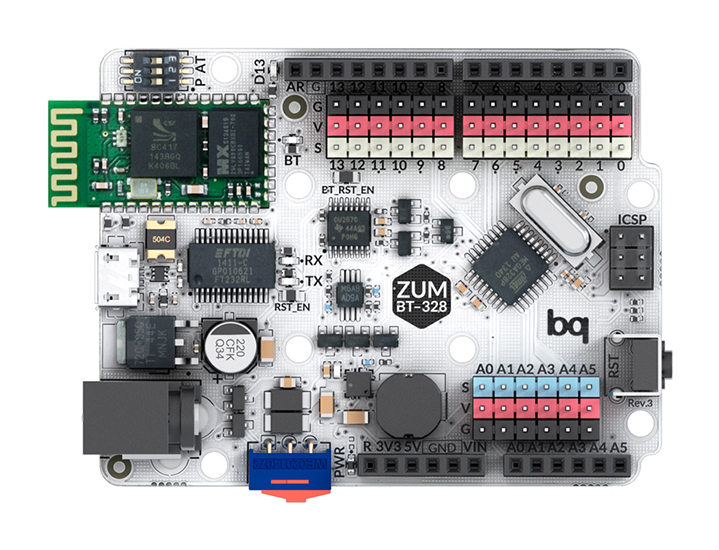
\includegraphics[width=0.6\textwidth]{Figures/BQZUM}
\caption[BQ Zum Bluetooth empleada para mover los servos]{BQ Zum Bluetooth empleada para mover los servos}
\label{fig:BQZUM}
\end{figure}


%-----------------------------------
%	SUBSECTION 1: VISIÓN
%-----------------------------------
\subsection{Cámara visión por computador}

Se realiza una prueba piloto aprovechando el sistema de visión instalado para otro proyecto, compuesto por la cámara fija de Fanuc, 2 paneles LED de luz difusa (60W) y el software de visión Fanuc: iRvision. Se elige realizar las pruebas en ésta plataforma, y no en un ordenador convencional con matlab u opencv, por inmediatez, el sistema está ya calibrado y en funcionamiento, además de que cuenta con un rack de salidas y entradas digitales; como se ha dicho, el objetivo era comprobar la viabilidad.

El sistema de visión está conectado al controlador de un brazo robótico LRMate 200iD, con un módulo I/O digitales a 24 voltios. Por lo que se realiza una interfaz con 2 relés para comunicar con la placa Arduino (5V), encargada de calibrar los servos del juguete.

En la figura \ref{fig:CeldaFanuc} podemos ver el área de trabajo de la celda robótica y su cámara.

\begin{figure}
\centering
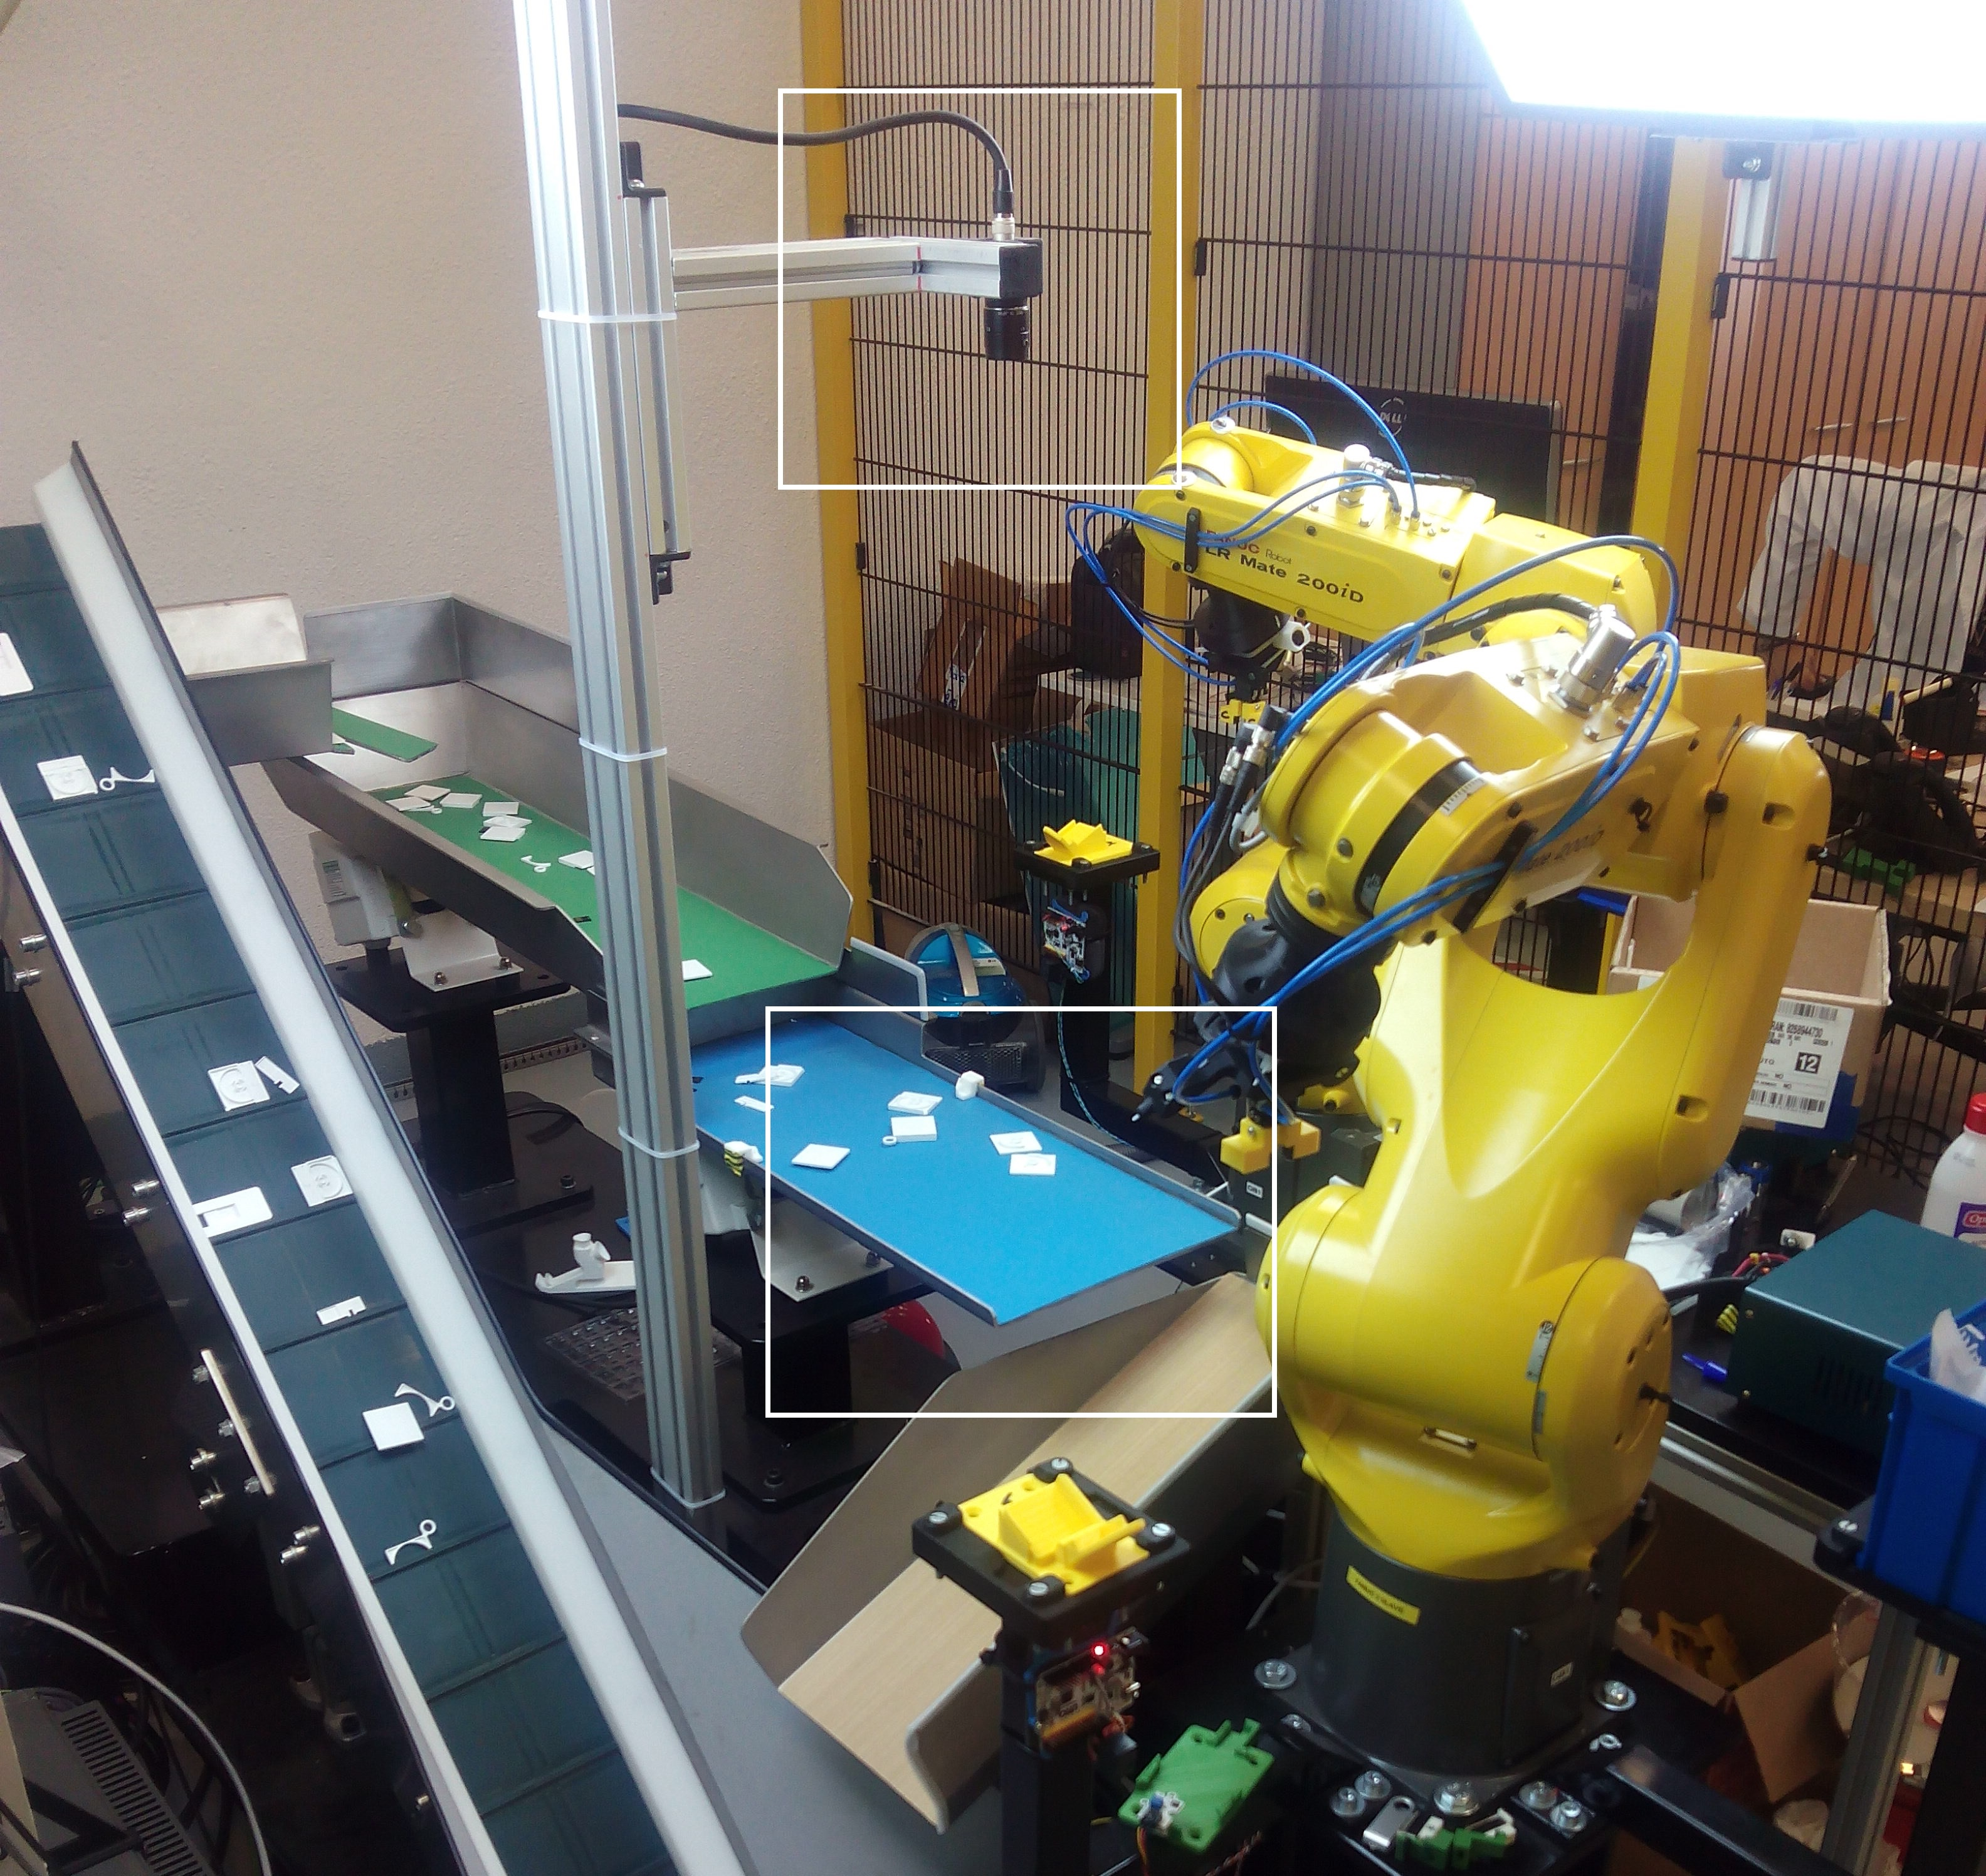
\includegraphics[width=120mm]{Figures/CeldaFanuc}
\caption[Celda con cámara de Fanuc]{Celda con cámara de Fanuc}
\label{fig:CeldaFanuc}
\end{figure}

El programa creado en Arduino recibe como entradas dos señales que indican en qué sentido se debe girar el servo. Como salida, actúan sobre el servo hacíendolo corregir su posición iterativamente 1 grado cada segundo hasta alcanzar la posición deseada.

La posición deseada es definida utilizando iRvision (Software de visión de Fanuc), mediante técnicas de visión por computador (Localización de elementos entrenados, medición de distancias y ángulos entre ellos). Para el caso del "tobillo", buscando perpendicularidad con la "cadera", y para ésta, consiguiendo cierta distancia entre dos líneas paralelas. Se pueden ver las Figuras \ref{fig:Tobillo} y \ref{fig:Cadera}.

\begin{figure}
\centering
\begin{minipage}{.5\textwidth}
  \centering
  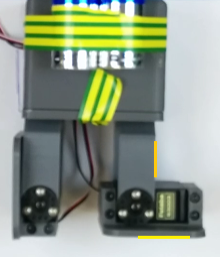
\includegraphics[width=.7\textwidth]{Figures/Tobillo}
  \captionof{figure}{Calibración tobillo con visión}
  \label{fig:Tobillo}
\end{minipage}%
\begin{minipage}{.5\textwidth}
  \centering
  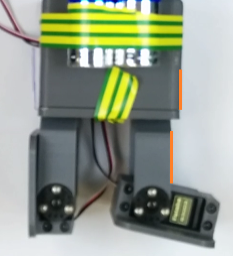
\includegraphics[width=.7\textwidth]{Figures/Cadera}
  \captionof{figure}{Calibración cadera con visión}
  \label{fig:Cadera}
\end{minipage}
\end{figure}


%-----------------------------------
%	SUBSECTION 2: IMUS
%-----------------------------------

\subsection{Sensores IMUs}
Para la segunda prueba se emplea una placa que combina un giróscopo, acelerómetro y magnetómetro para formar una unidad de medición inercial (de ahora en adelante IMU) con una precisión de hasta 0.1 grados.

\subsubsection{Teoría}

La MinIMU-9 v3 (Figura \ref{fig:MinIMU_board} fue seleccionada de entre varias opciones, como la famosa MPU6050, la GY-87 o la versión v2 de MinIMU (todas de un precio similar), por la precisión y repetibilidad de las lecturas, además de parecer un dispositivo ampliamente utilizado y probado por la comunidad.

\begin{figure}
\centering
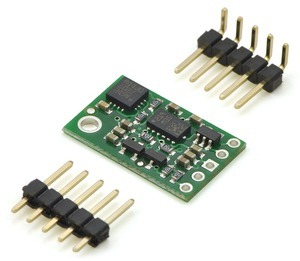
\includegraphics[width=65mm]{Figures/MinIMU_board}
\caption[MinIMU-9 v3 de Pololu]{MinIMU-9 v3 de Pololu}
\label{fig:MinIMU_board}
\end{figure}

Tras estudiar el comportamiento del sensor, y una fase de documentación acerca de las opciones de que se dispone, surgen tres posibilidades:

\begin{itemize}
  \item Librería de Pololu "MinIMU-9 AHRS"
  \item Librería "Open IMU"
  \item Desarrollar la matemática tomando los valores RAW del sensor
\end{itemize}

A pesar de lo atractivo de la tercera opción, no se disponía de suficiente tiempo para seguir adelante con ella, se trató de comprender el funcionamiento de las 2 librerías ya creadas.

Por simplicidad, Open IMU resultaba llamativa, pero rápidamente se percibió que podía quedarse demasiado corta y que las lecturas obtenidas empleando ésta librería (los ángulos euler de pitch, roll y yaw) parecían no tener la repetibilidad necesaria para nuestra aplicación, por otro lado, hacía más de 3 años que no se realizaban cambios en su repositorio GIT, por lo que posiblemente estaba preparada para funcionar con la versión anterior de la placa, MinIMU-9 v2, con una exactitud de hasta 1 grado solamente.

La línea elegida fue la de la librería recomendada por Pololu (fabricante del dispositivo), dejando un poco limitado el modo de funcionar pero ofreciendo un acceso rápido a las mediciones del sensor en forma de posición en ángulos euler.

Para un correcto funcionamiento del magnetómetro, se han de configurar los valores máximos y mínimos de las lecturas del acelerómetro, estos 2 sensores se encuentran en el encapsulado LSM303, la librería de dicho chip proporciona un programa de Arduino que captura dichas mediciones y salva la mayor mientras movemos la placa en todas las orientaciones posibles, mostrandola por el puerto serie. Los valores obtenidos se han de escribir, sustituyendo los "por defecto", en la cabecera de la misma librería.

La limitación de ésta librería que se había comentado antes , es que para obtener con precisión los ángulos euler en todas las orientaciones, se debe llamar una función de la librería \textbf{calibrateIMU()} con la placa colocada en una de las 2 posiciones que se ven en la Figura \ref{fig:IMU_positions}, lo más paralelo al suelo posible, con ésta función definimos en el espacio el 0 de los ejes X e Y del sistema, por lo que se corrigen desvíos si la posición no es totalmente horizontal, sin embargo, ésto deriva en errores que crecen en proporción a la inclinación que se de en alguno de los ejes. Se elige una de ellas configurando ciertos parámetros de la librería de Pololu en el programa principal.

\begin{figure}
\centering
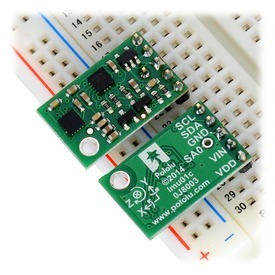
\includegraphics[width=65mm]{Figures/IMU_positions}
\caption[Posiciones calibración IMU]{Posiciones calibración IMU}
\label{fig:IMU_positions}
\end{figure}

La orientación en Z depende de la brújula y su tiempo de estabilización es lento, por ello, se piensa en emplear los giros en los otros 2 ejes, X e Y, por lo que la posición del robot ha de ser la de acostado sobre un lado, descartando las posiciones que, de entrada, parecen más razonables como boca arriba/boca abajo, o con las piernas hacia arriba. Ver Figuras \ref{fig:patas_arriba} y \ref{fig:acostado}.

\begin{figure}
\centering
\begin{minipage}{.5\textwidth}
  \centering
  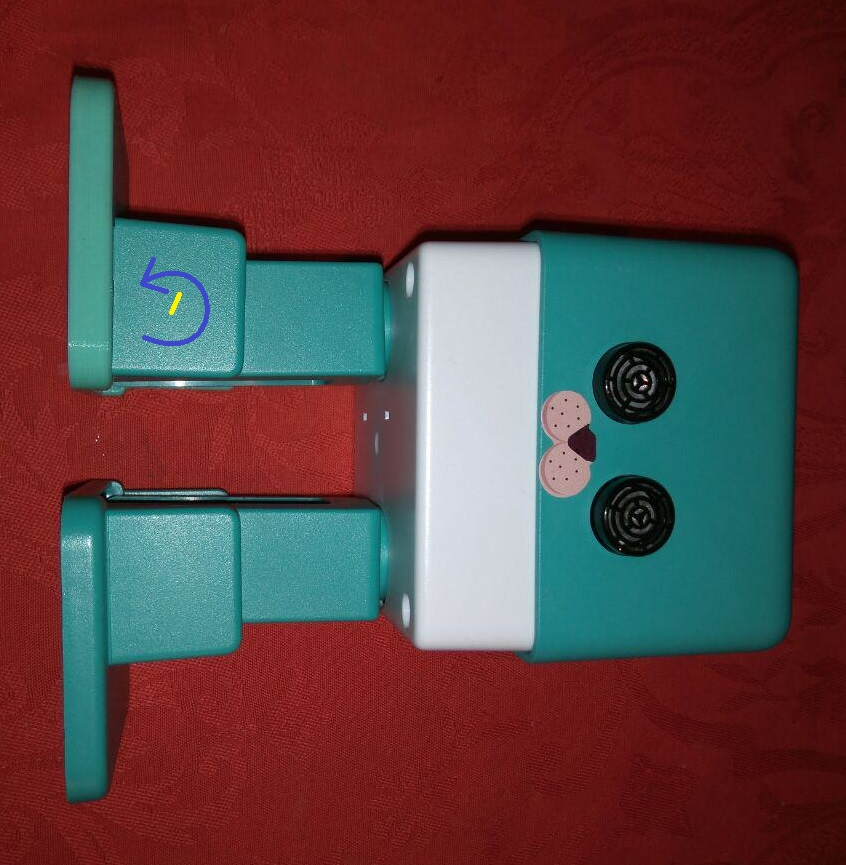
\includegraphics[width=.9\textwidth]{Figures/acostado}
  \captionof{figure}{Tobillo gira sobre eje Z}
  \label{fig:acostado}
\end{minipage}%
\begin{minipage}{.5\textwidth}
  \centering
  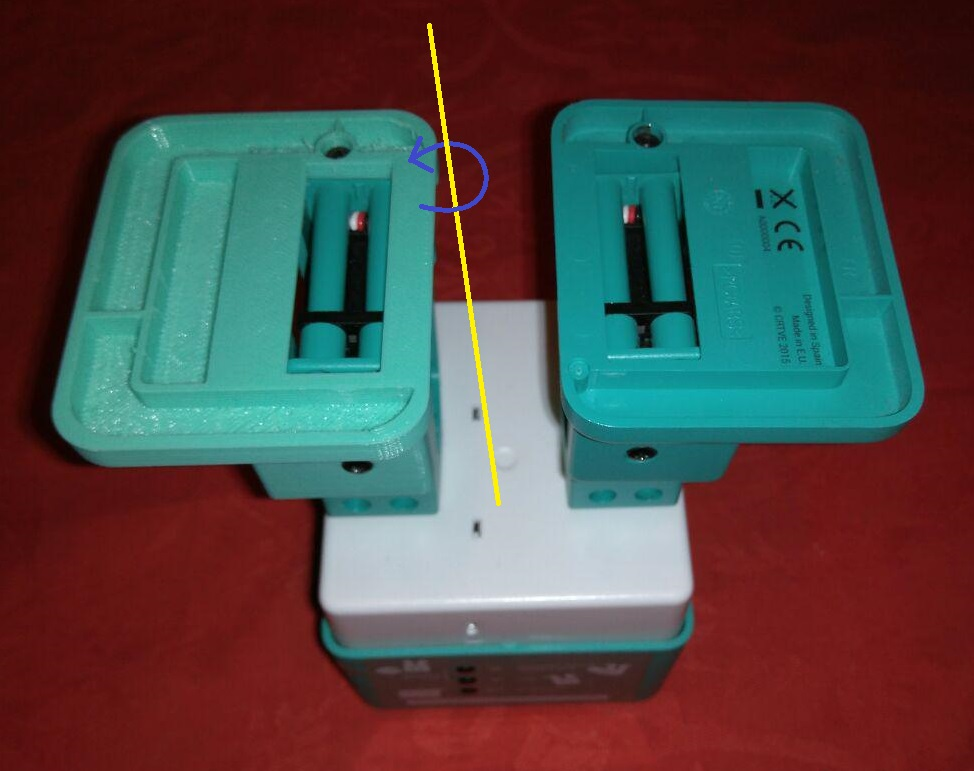
\includegraphics[width=.9\textwidth]{Figures/patas_arriba}
  \captionof{figure}{Cadera gira sobre eje Z}
  \label{fig:patas_arriba}
\end{minipage}
\end{figure}


\subsubsection{Prueba inicial}

Se programa el algoritmo empleando una máquina de estados en la misma placa controladora de Zowi con un pulsador para pasar de un estado a otro. Versión muy básica para probar el concepto. Se emplea comunicación serie para conocer el estado del sensor y una grapa impresa para acoplarlo al pié del Zowi.

El procedimiento programado sería:
\begin{itemize}
  \item Iniciar el sistema -- Automáticamente se produce la calibración de la IMU
  \item Colocar el sensor en el pié de Zowi
  \item Pulsar el botón -- Se inicia la calibración del servo
\end{itemize}

El modo de calibración del servo consiste en dar un primer valor a la posición que debería tener el servo, es decir, 0º para la cadera o 90º para el pie, entonces se lee el sensor para ver el error cometido y se ajusta la posición del servo teniendo en cuenta la diferencia del valor deseado y la nueva lectura, se repite hasta 2 veces.

Se obtienen buenas sensaciones con éste método y se nota de inmediato que el éxito del mismo radica en la correcta calibración inicial del sensor y en una buena fijación al pié del robot, por lo que se desarrolla un zapato para montar en él el sensor y un soporte para el robot, junto a otro soporte para realizar la calibración del sensor (ya integrado en el zapato) en la misma pieza. De esta forma se garantiza la correspondencia y paralelismo de los planos de apoyo de ambas partes (robot – zapato).

%-----------------------------------
%	Conclusiones
%-----------------------------------

\subsection{Conclusiones}
El método de calibración empleando visión muestra buenos resultados y es muy mejorable si se emplea software creado específicamente para la aplicación, sin embargo, las condiciones de iluminación y posición han de ser las mismas o muy parecidas para cada banco de trabajo para garantizar un buen funcionamiento del software, por lo que su instalación, puesta en marcha y configuración, son delicados y se deberían hacer in-situ. En el momento de las pruebas de validación aún se desconoce la ubicación de la fábrica y la nave de montaje -posiblemente en China o Polonia-,  la solución se encarece considerablemente si se han de realizar desplazamientos para llevar a cabo la instalación y puesta en marcha.

Con las IMUs se obtuvieron buenos resultados y se tenía bastante claro que se quería seguir adelante con ellas por su bajo coste y y su fácil implementación. Quedaba afinar el algoritmo de calibración implementando una máquina de estados mucho más robusta y endureciendo el criterio de validación automática de una buena calibración para obtener mejores resultados. En el siguiente subcapítulo se desarrolla su evolución.

%----------------------------------------------------------------------------------------
%	SECTION 3: Laboratorio
%----------------------------------------------------------------------------------------

\section{Prototipo de laboratorio}

Se decide continuar con la solución de las IMUs y se producen reuniones cada pocos días/semanas entre los diferentes grupos implicados en el desarrollo del juguete Zowi (mecánica, hardware, producto, automatización...) dónde las especificaciones el banco de calibración van tomando forma en función de los resultados obtenidos. En la presente sección se mostrará la línea de evolución del prototipo, mencionando las características y mejoras más relevantes añadidas, así como las pruebas realizadas antes de pasar al desarrollo de la versión final.

\subsection{Línea de evolución}

Tras elegir la línea de los sensores IMU, se comienza a trabajar de inmediato en la mejora de la solución.

\subsubsection{Primeras mejoras}

La máquina de estados es mejorada, diferenciando calibraciones malas de calibraciones buenas. Se añaden una indicador led y uno acústico para resaltar el resultado con diferentes sonidos. Esta mejora se mantendrá hasta la versión final del producto.

La siguiente necesidad a cubrir sería garantizar que el robot comparte el plano con el sensor, que ha de ser calibrado antes de colocarse en el robot como explicamos en la sección anterior. Hasta ahora el sensor era fijado utilizando una grapa impresa (Ver Figura \ref{fig:grapa}).

\begin{figure}[h]
\centering
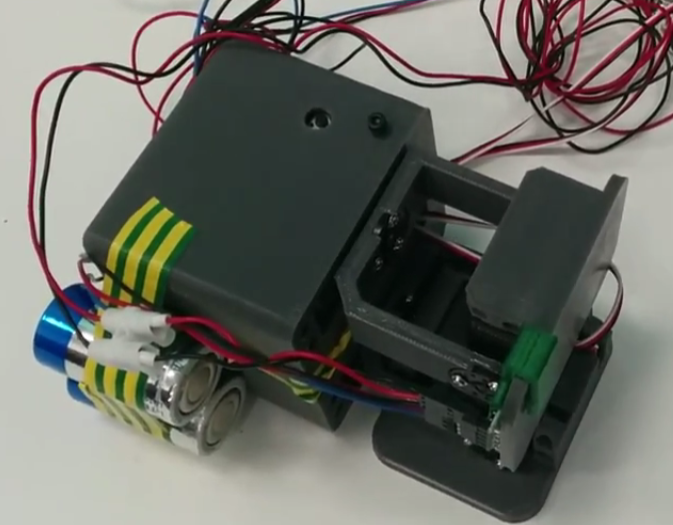
\includegraphics[width=70mm]{Figures/grapa}
\caption[Sensor anclado con grapa impresa]{Sensor anclado con grapa impresa}
\label{fig:grapa}
\end{figure}

Se monta el sensor en una pieza especialmente diseñada e impresa para colocarla en el pié de Zowi, razón por la que es llamada "Zapato".
Se crea también una base donde se coloca el Zowi, con un área para colocar el zapato en el momento de su inicialización, dónde el sensor es calibrado. Se puede ver el banco en la Figura \ref{fig:banco_1zapato}.


\begin{figure}[h]
\centering
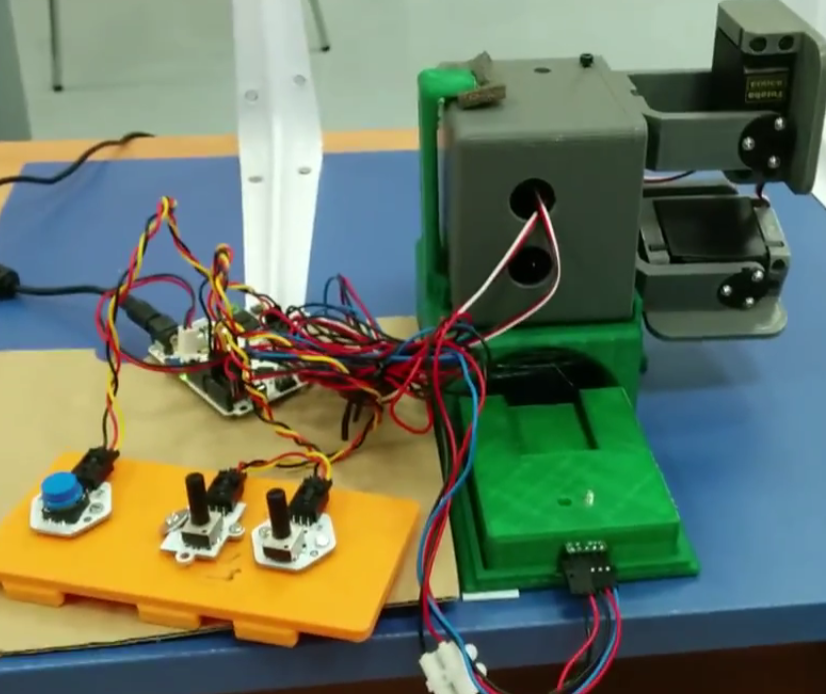
\includegraphics[width=80mm]{Figures/banco_1zapato}
\caption[Bancos impresos para Zowi y zapato]{Bancos impresos para Zowi y zapato}
\label{fig:banco_1zapato}
\end{figure}

El algoritmo hasta ahora pasaba por calibrar una pierna del juguete solamente, haciendo ambas partes -tobillo y cadera-. Se mejora este punto, conectando a la placa controladora 2 sensores IMUs. La comunicación con la MinIMU-9 se realiza a través de I\textsuperscript{2}C, y su interfaz permite seleccionar facilmente entre 2 direcciones distintas para el giróscopo, y lo mismo para el acelerómetro/brújula. Para ello solamente tenemos que conectar SA0 a GND. (Ver Figura \ref{fig:minimu_sa0} y Tabla \ref{tablei2c})

\begin{table}[h]
\centering
\begin{tabular}{l c c}
\toprule
\textbf{Sensor} & \textbf{Slave Add. - default} & \textbf{Slave Add. - SA0 driven low} \\
\midrule
L3GD20H (gyro) & 1101011b & 1101010b \\
LSM303D (acc+magnet) & 0011101b & 0011110b \\
\bottomrule\\
\end{tabular}
\caption{Direcciones de esclavo I\textsuperscript{2}C para MinIMU-9 v3}
\label{tablei2c}
\end{table}

\begin{figure}[h]
\centering
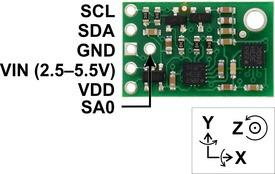
\includegraphics[width=60mm]{Figures/minimu_sa0}
\caption[MinIMU-9 v3 Pin-out]{MinIMU-9 v3 Pin-out}
\label{fig:minimu_sa0}
\end{figure}

Es necesario cambiar las direcciones de una de las placas, de lo contrario ambas tendrían las mismas direcciones de esclavo I\textsuperscript{2}C y causaría un mal funcionamiento el intentar leer de una de ellas. Además, se mejora el banco impreso para poder albergar los 2 zapatos y la máquina de estados, implementando la calibración de ambas piernas y aumentando número de iteraciones e incluyendo un filtrado de múltiples medidas para evitar leer ruido. Ver Figura \ref{fig:banco_2zapato}.

\begin{figure} [h]
\centering
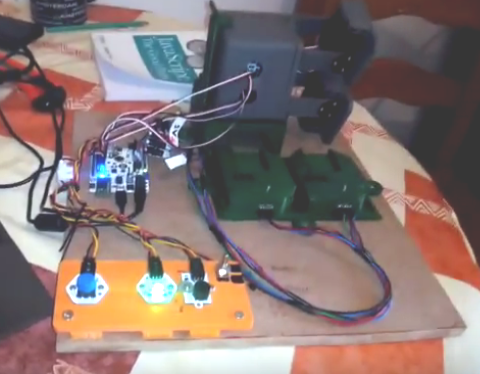
\includegraphics[width=70mm]{Figures/banco_2zapato}
\caption[Banco 1 zapato]{Banco impreso para Zowi y 2 zapatos}
\label{fig:banco_2zapato}
\end{figure}

La calibración/inicialización de los sensores muestra resultados, como se ha comentado anteriormente, no tan buenos cuando el sensor se inclina notablemente. Por ello que el éxito de la calibración de la cadera (0º de set point) es mayor que el de la calibración del pié (90º). Se considera corregir el set point de los piés en la fase de calibración de los sensores.

Se diseñan unos cajetines para el ajuste del sensor a los 90º, de modo que antes de comenzar la calibración de los juguetes, el sensor (zapato), debe ser calibrado en las posiciones horizontal y vertical.

Se impide avanzar en el procedimiento si tras calibrar los sensores al inicio, las medidas obtenidas difieren demasiado de 0º en ambos ejes, se vuelve a un estado en el que se espera pulsar el botón para volver a realizar la calibración, es decir, se comienza a implementar una gestión de errores.

Se añaden al conjunto un nivel y unos tornillos para regular la inclincación y mantener todo lo más horizontal posible antes de comenzar. Ver Figura \ref{fig:banconivel}.

\begin{figure}
\centering
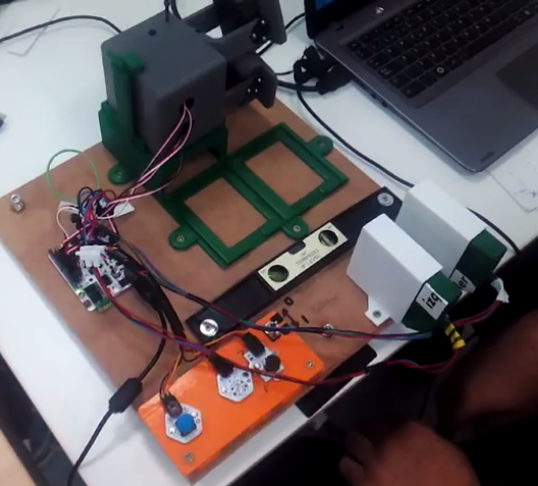
\includegraphics[width=80mm]{Figures/banco_nivel}
\caption[Banco con inclinación regulable]{Banco con inclinación regulable}
\label{fig:banconivel}
\end{figure}

%-----------------------------------
%	SUBSUBSECTION 1
%-----------------------------------
\subsubsection{Tomando forma}

Hasta ahora todas las pruebas se habían realizado en la misma controladora de Zowi. Se recibe información sobre la placa que será empleada para los robots (en desarrollo por el Dpto. de Hardware), se conoce que el número de entradas/salidas será reducido y ajustado a los sensores/actuadores del propio juguete, por lo que realizar todas las conexiones que planteamos en nuestras pruebas en la misma placa junto a todos los periféricos de zowi no es una opción.

Se plantea el uso de otra placa conectada por I\textsuperscript{2}C a la placa controladora del Zowi (por ahora una ZUM BT) y la librería Wire.h de Arduino. Zum BT es una versión de la Arduino UNO con bluetooth incorporado, y una etapa de potencia capaz de sacar hasta 3.2 amperios por sus salidas digitales.

La nueva placa empleada sería una Freeduino Mega, versión basada en la Mega, es elegida por ser compatible con todo lo desarrollado y por su bajo coste para la empresa y por presentar una cantidad de entradas y salidas mayor que los modelos UNO.

Se vuelven a diseñar unos bancos para calibrar los sensores tanto horizontal como verticalmente, es decir, inicializar ejes y ajustar el eje Y en vertical. Todo en el mismo espacio, como se puede ver en la Figura \ref{fig:bancov3}.

\begin{figure}
\centering
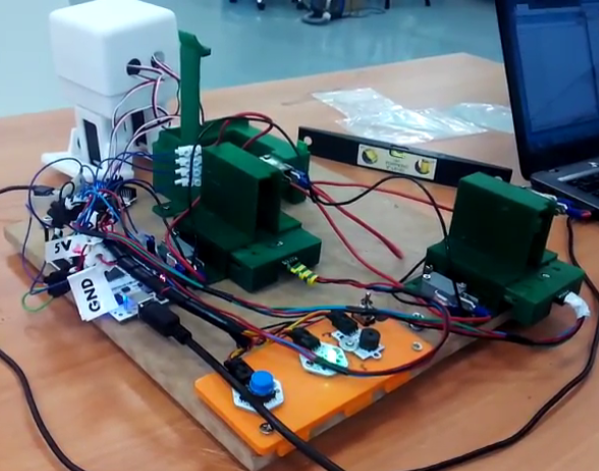
\includegraphics[width=110mm]{Figures/banco_v3}
\caption[Banco con conexión MEGA-ZUM]{Banco con conexión MEGA-ZUM}
\label{fig:bancov3}
\end{figure}

El empleo de una Mega nos proporciona una gran cantidad de pines de entrada salida, se incorporan al sistema unos finales de carrera para detectar que los zapatos están en la posición correcta para su calibración.

Como característica \textbf{principal}, se diseña una interfaz de comunicación entre ambas placas mediante I\textsuperscript{2}C, se construyen determinadas "instrucciones" en la placa Mega (placa con la máquina de estados) y un programa que funciona como intérprete que es cargado en la ZUM (placa del robot), se encarga de traducir las instrucciones recibidas de la otra placa por I\textsuperscript{2}C en movimientos de servos, entre otras cosas. Puede verse la arquitectura del sistema en la Figura \ref{fig:v3-diag}.

\begin{figure}
\centering
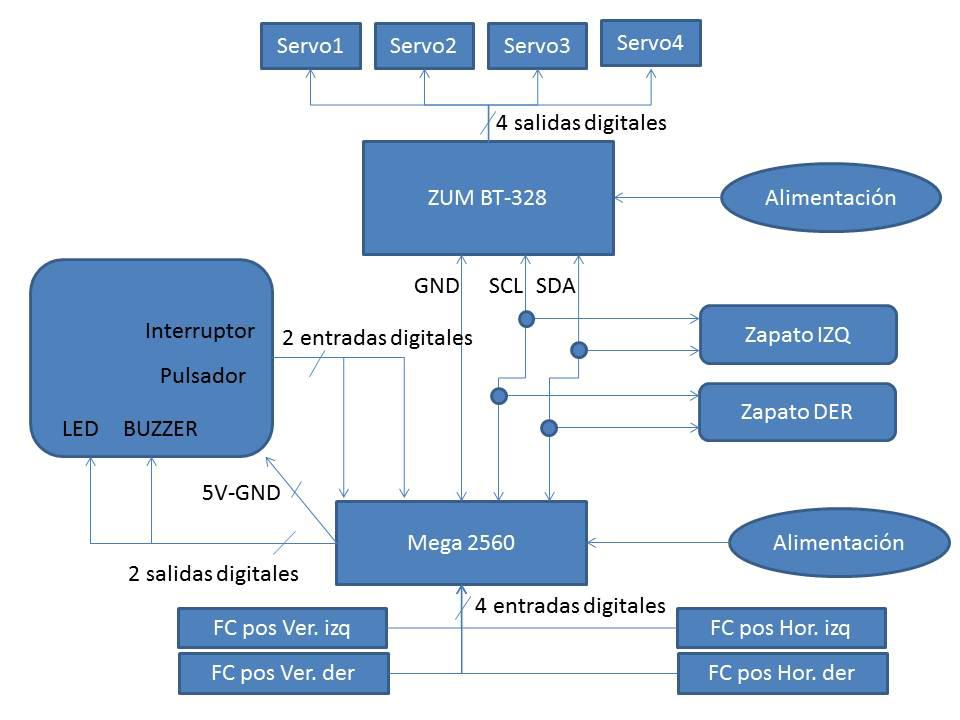
\includegraphics[width=130mm]{Figures/v3-diag}
\caption[Arquitectura versión MEGA-ZUM por I\textsuperscript{2}C]{Arquitectura versión MEGA-ZUM por I\textsuperscript{2}C}
\label{fig:v3-diag}
\end{figure}

La máquina de estados se hace más robusta en general, detectando fallos y facilitando la recuperación para un correcto funcionamiento.

Al final de esta etapa se conoce la controladora que llevará el juguete, así como la versión -prototipo- de Zowi definitiva, sinterizada por láser, en lugar de inyectada, pero ya con sus dimensiones y forma finales. Se puede ver en la Figura \ref{fig:zowi-sls}.

\begin{figure}
\centering
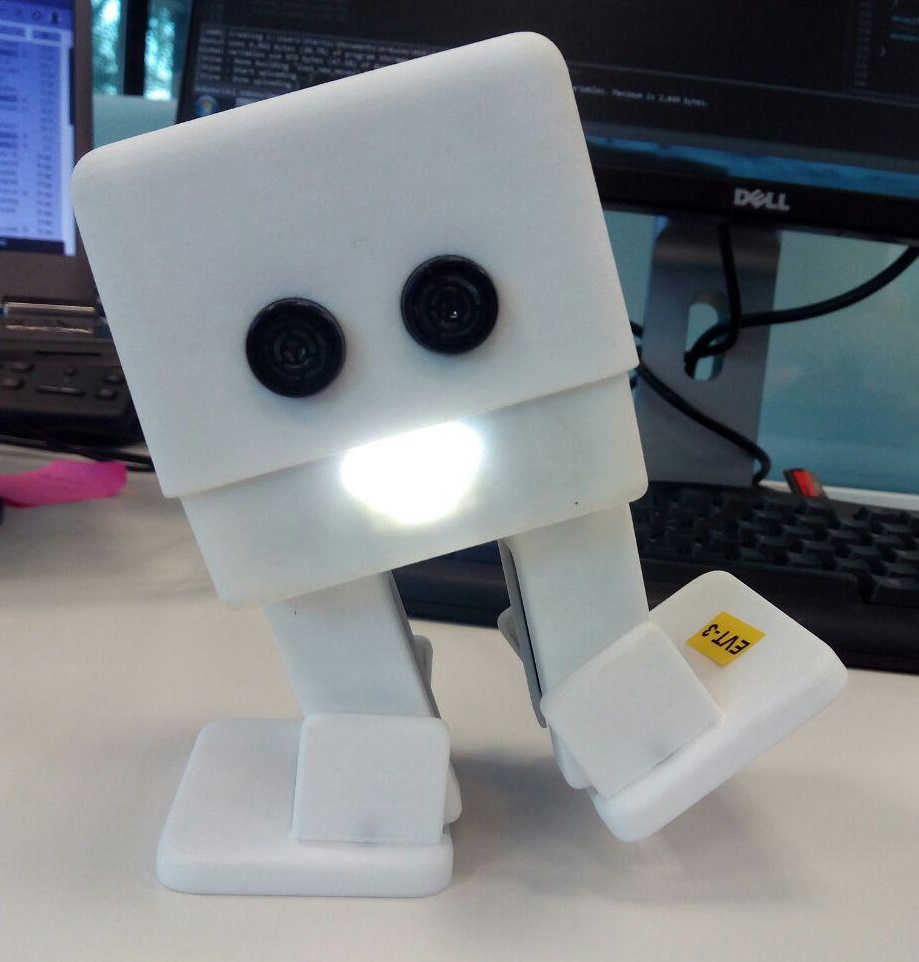
\includegraphics[width=90mm]{Figures/zowi-sls}
\caption[Prototipo final Zowi SLS]{Prototipo final Zowi SLS}
\label{fig:zowi-sls}
\end{figure}

\subsubsection{Prototipo final: Banco de Calibración}

En este punto se produce el mayor cambio en el proyecto. La solución de comunicación por I\textsuperscript{2}C entre las diferentes placas asumía que la controladora de Zowi tendría accesibles los pines al micro para I\textsuperscript{2}C y SPI (cosa incierta) y, además, hacía necesario el acceso al interior del robot, que en principio, podría llegar ya montado de las etapas de producción anteriores. Se sugiere implementar la comunicación a través del puerto USB que tendrá la placa de Zowi.

Las controladoras Arduino pueden ser esclavos serie por USB, no maestros, realizar una comunicación serie de una a otra no es posible, de ahí que se plantee usar una Raspberry PI (Figura \ref{fig:raspi}) como maestro Serie de ambas placas, esclavos serie, sustituyendo la interfaz I\textsuperscript{2}C implementada en la versión anterior y haciendo de puente entre ambas.

Se contempló la posibilidad de quitar la Mega y emplear solamente la Raspberry como núcleo del sistema, sin embargo, eso conllevaría rehacer gran parte del trabajo y encontrar la forma de hacer funcionar los sensores con éste dispositivo, lo que requería un tiempo que no se tenía.

Una primera iteración fue la de sustituir la comunicación por I\textsuperscript{2}C, por la comunicación serie, se adaptaron los programas de MEGA y de ZUM. La comunicación era unidireccional. Mega > Raspberry > Zowi. La Raspberry PI funcionaba como mero driver de comunicaciones:
\begin{itemize}
  \item Se modificaron los comandos enviados con la librería Wire.h desde la freeduino Mega para ser comandos enviados por serie (Librería Serial.h) con ciertos caracteres de inicio y fin de comunicación a modo de protocolo (desarrollado específicamente para esta aplicación).
  \item Se implementó en la Raspberry un programa en Python que hacía de intérprete. Haciendo escucha a la comunicación serie abierta con la Freeduino Mega, y enviando comandos a la placa controladora de Zowi a través de la comunicación Serie abierta con ella.
\end{itemize}

La incorporación al sistema de una Raspberry PI, un ordenador al fin y al cabo, abría gran cantidad de mejoras de fácil implementación, por lo que se aprovechó la ocasión para desarrollar un prototipo "casi definitivo", no solamente a nivel de software.

Se decide introducir la electrónica en un armario eléctrico y, a su vez, emplear el mismo como estructura del soporte de Zowi y de los zapatos. Ver Figura \ref{fig:bancov4}. Se integran nivel y patas regulables.

\begin{figure}
\centering
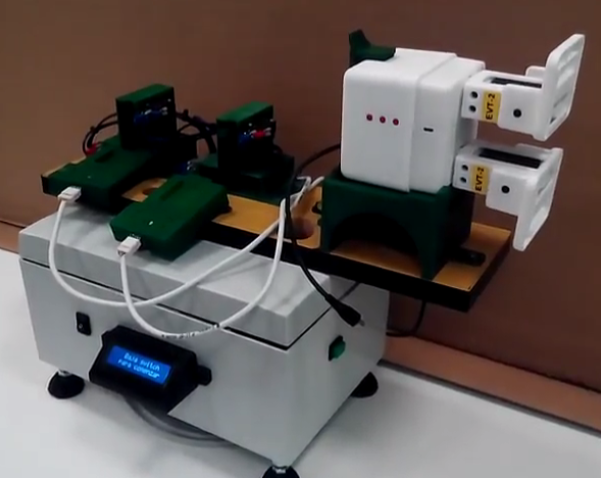
\includegraphics[width=110mm]{Figures/banco_v4}
\caption{Banco prototipo final}
\label{fig:bancov4}
\end{figure}

Se introdujo un display LCD conectado a la Mega por I\textsuperscript{2}C que hacía más fácil la interacción del usuario con el banco de calibración y se trabajó en mejorar la máquina de estados para hacer el uso del sistema más amigable; y se mejoró el conexionado añadiendo una PCB custom como shield de la Mega, que ofrecía borneros para conectar los leds, display LCD, IMUs, finales de carrera y botones.

Durante el proceso de calibración se guardarán los offsets calculados en ciertas posiciones de la memoria EEPROM de la placa controladora de Zowi. Se usa para ello la librería EEPROM.h. Esto es necesario para el funcionamiento de los programas por defecto, cuyas librerías (zowi.h y oscillator.h) están configuradas para usar los valores en dichas posiciones de la memoria.

Multitud de mejoras software definitivas fueron implementadas en esta fase para aumentar su funcionalidad, en el subcapítulo siguiente se verán en mayor detalle, a destacar:
\begin{itemize}
  \item Raspberry utilizada como programador, empleando la utilidad AVRDUDE cargará el programa de calibración en cada Zowi.
  \item Cargará, del mismo modo y al finalizar la calibración, el programa de fábrica con que saldrá a la venta el producto. Sobrescribiendo el de calibración.
  \item Se le habilita acceso remoto por SSH y por XRDP para poder acceder a ella desde fuera.
  \item Se instala un servidor de MySQL y se configura para guardar datos tanto en local como en nuestros servidores.
  \item El entorno de programación de Arduino es instalado, para poder modificar la Mega directamente desde Raspberry.
\end{itemize}

%-----------------------------------
%	SUBSECTION 2
%-----------------------------------

\subsection{Pruebas realizadas}


Durante todo el desarrollo se han realizado pruebas, sin embargo, se comentan los resultados la prueba previa a MP (massive production), realizada con el prototipo final. La Figura \ref{fig:pre-mp} muestra el armario de calibración preparado para la prueba.

Los operadores fueron compañeros que no habían tenido contacto alguno con la máquina, haciendo de operarios de forma distraída.
\begin{figure}
\centering
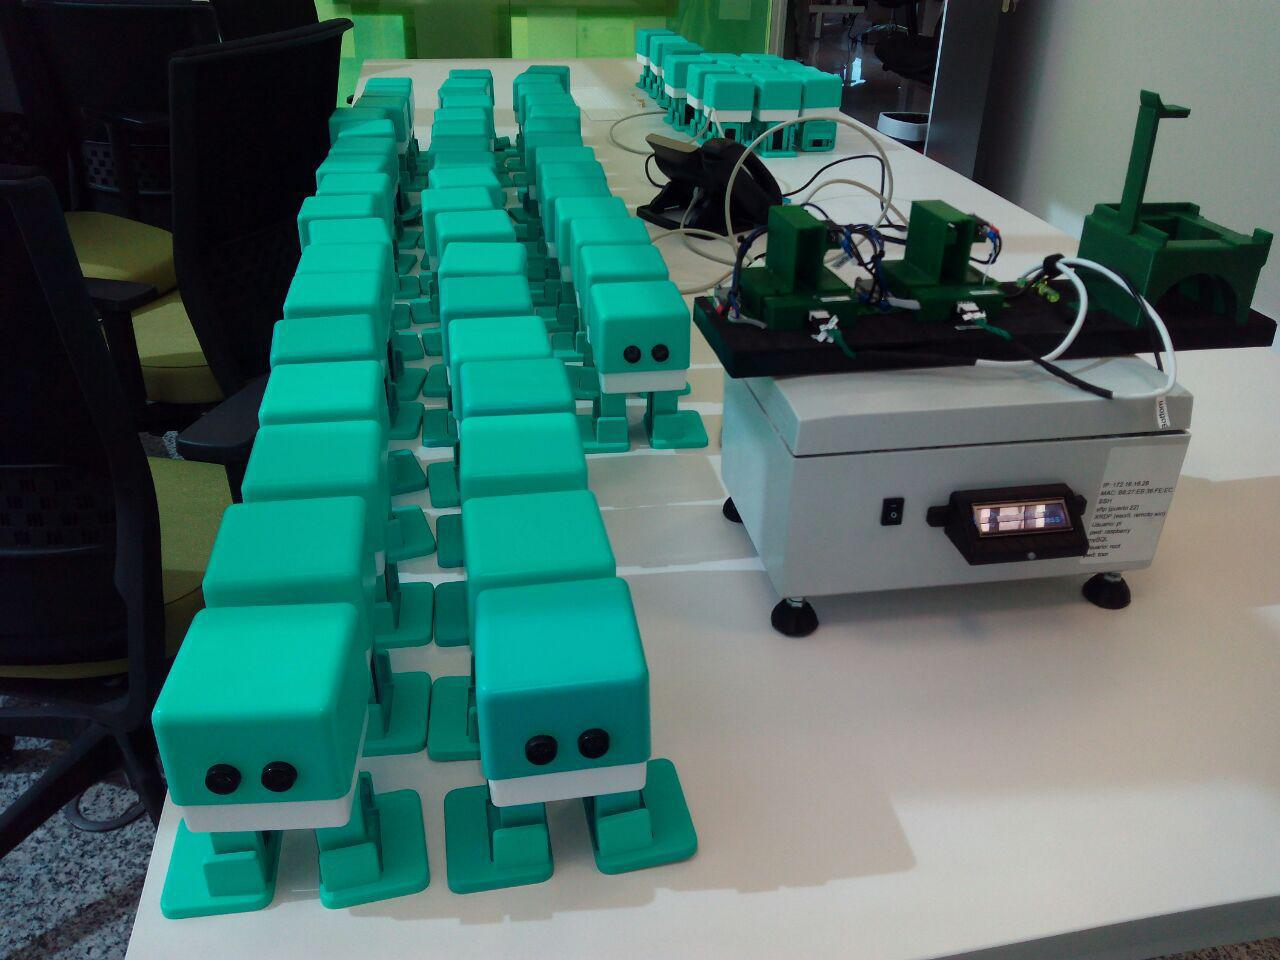
\includegraphics[width=110mm]{Figures/pre-mp}
\caption{Prueba pre MP}
\label{fig:pre-mp}
\end{figure}

Se logran calibrar satisfactoriamente 62 juguetes, con solamente 1 contratiempo: Al no respetar el protocolo en cuanto a órden de operaciones, concretamente, intento de programar la placa sin energizar. Si se intenta programar la placa conectada pero sin encender, el programador AVRDude realiza hasta 10 intentos de programarla sin éxito; al energizarla durante los intentos, según en qué momento se haga, puede ser recuperable, o puede llevar al sistema a un estado de fallo. Se tuvo que reiniciar y volver a hacer la calibración de los zapatos. A pesar de ser un error de operador, se intenta corregir para la versión final.

Un total de 4 veces se produce una calibración mala, inducidas para poner a prueba el sistema, el sistema notifica (Display y sonido) la calibración como mala y se necesita que se vuelva a pulsar el botón. De ahí una calibración de apenas unos segundos en las gráficas siguientes, por no tener que conectar y calzar al juguete).

Analizando la información extraída de la base de datos tras las calibraciones, se muestra (Figura \ref{fig:tiempos}) Segundos vs. n\textsuperscript{o} Zowi, una segunda gráfica (Figura \ref{fig:ok-nok}) muestra 1 para calibraciones válidas, 0 para las declaradas fallidas. Los tiempos del primer y último registro no son representativos.

\begin{figure}
\centering
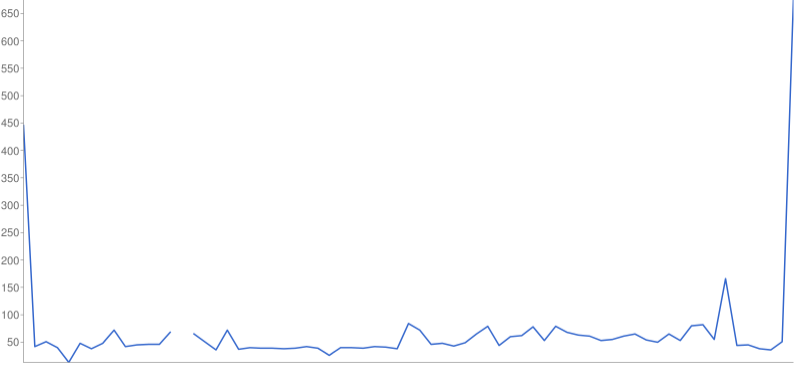
\includegraphics[width=140mm]{Figures/tiempos}
\caption{Segundos por cada calibración de Zowi}
\label{fig:tiempos}
\end{figure}

\begin{figure}
\centering
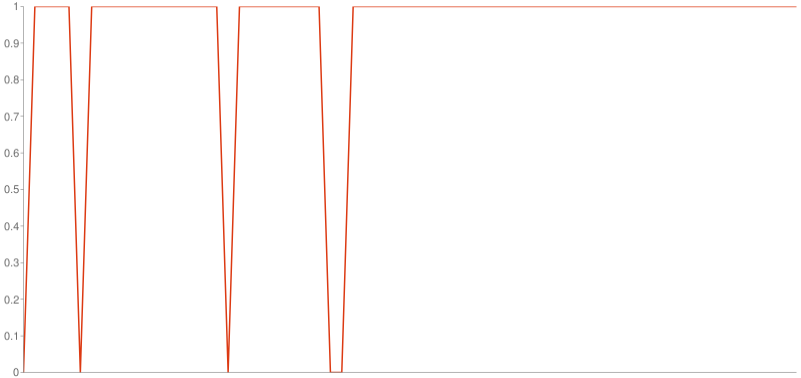
\includegraphics[width=140mm]{Figures/ok-nok}
\caption{OK:1 | NOK:0 - para cada calibración de Zowi}
\label{fig:ok-nok}
\end{figure}

%----------------------------------------------------------------------------------------
%	SECTION 4: Finales
%----------------------------------------------------------------------------------------

\section{Armarios finales}

El trabajo asignado al autor del proyecto debió haber concluido con el prototipo presentado en el subcapítulo anterior, dejando por diseñar una versión definitiva de los soportes y zapatos del banco al Dpto. de Mecánica de BQ, y el montaje de tantos armarios y bancos como fuese necesario para abordar la producción de todos los juguetes a Rosti (empresa de extrusión de plásticos y montaje subcontratada en Polonia), encargados del ensamblado de los robots Zowi; sin embargo, se decidió realizar el montaje de 2 armarios con ligeras modificaciones y planos eléctricos para enviar a Polonia ya probados y validados. Ver armarios en Figura \ref{fig:armariosFinales}.

\begin{figure}
\centering
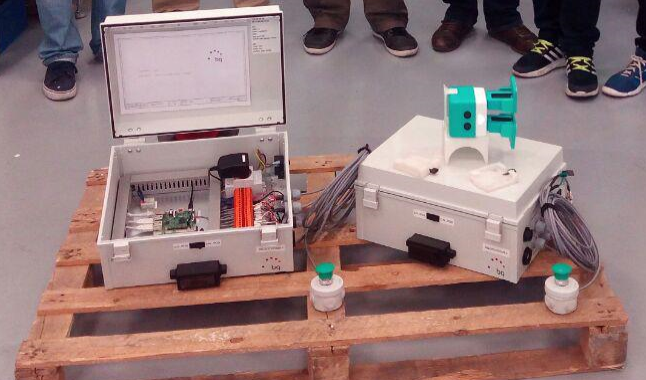
\includegraphics[width=110mm]{Figures/armariosFinales}
\caption{Armarios finales preparados para su envío a fábrica}
\label{fig:armariosFinales}
\end{figure}

Modificaciones destacables respecto al prototipo:
\begin{itemize}
  \item Armario de componentes eléctricos separado de la parte mecánica, se siguieron utilizando los diseños impresos de versiones anteriores para validación del funcionamiento, pero las piezas finales quedaban a cargo del Dpto. de Mecánica. Éste nuevo armario sería más amplio que el anterior.
  \item Mangueras de cables más largas (pues armario y banco de calibración irán separados).
  \item Pulsador exterior con una manguera de cable para ser colocado donde se desee en fábrica, en lugar del pulsador en el lateral del armario de la versión anterior.
  \item Conexión USB y Ethernet por pasamuros al interior del armario.
  \item Cambios en el diseño del cajetín del display LCD, pues el armario irá colocado a la altura de los ojos del operador.
\end{itemize}

%-----------------------------------
%	SUBSECTION 1
%-----------------------------------
\subsection{Componentes e implementación física}

\subsubsection{Arquitectura y conexiones}

El diagrama que se puede ver en la Figura \ref{fig:diagFinal}, muestra, a grandes rasgos, un esquema de las conexiones entre los principales dispositivos que intervienen en el sistema. El sistema completo consta del armario eléctrico, además del juguete Zowi conectado al armario. Por ello se muestran en el esquema tanto las placas internas del armario (Mega y Raspberry), como la placa controladora de Zowi (Zum).

\begin{figure}
\centering
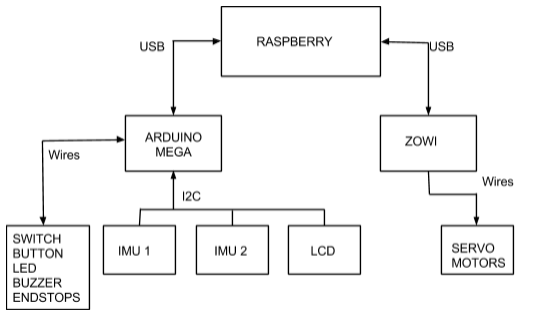
\includegraphics[width=100mm]{Figures/diagFinal}
\caption{Esquema de conexiones}
\label{fig:diagFinal}
\end{figure}

\subsubsection{Armario eléctrico}

Se elige instalar la parte fija del sistema en una placa de montaje dentro de un armario eléctrico de 40x30x18cm. Se emplean canaletas y bornas en un carril DIM para facilitar las conexiones al exterior del armario. Se utilizan pasamuros para las mangueras a pulsador y sensores IMU, así como para conexión USB (Raspberry - Zowi) y RJ45.

\begin{figure}
\centering
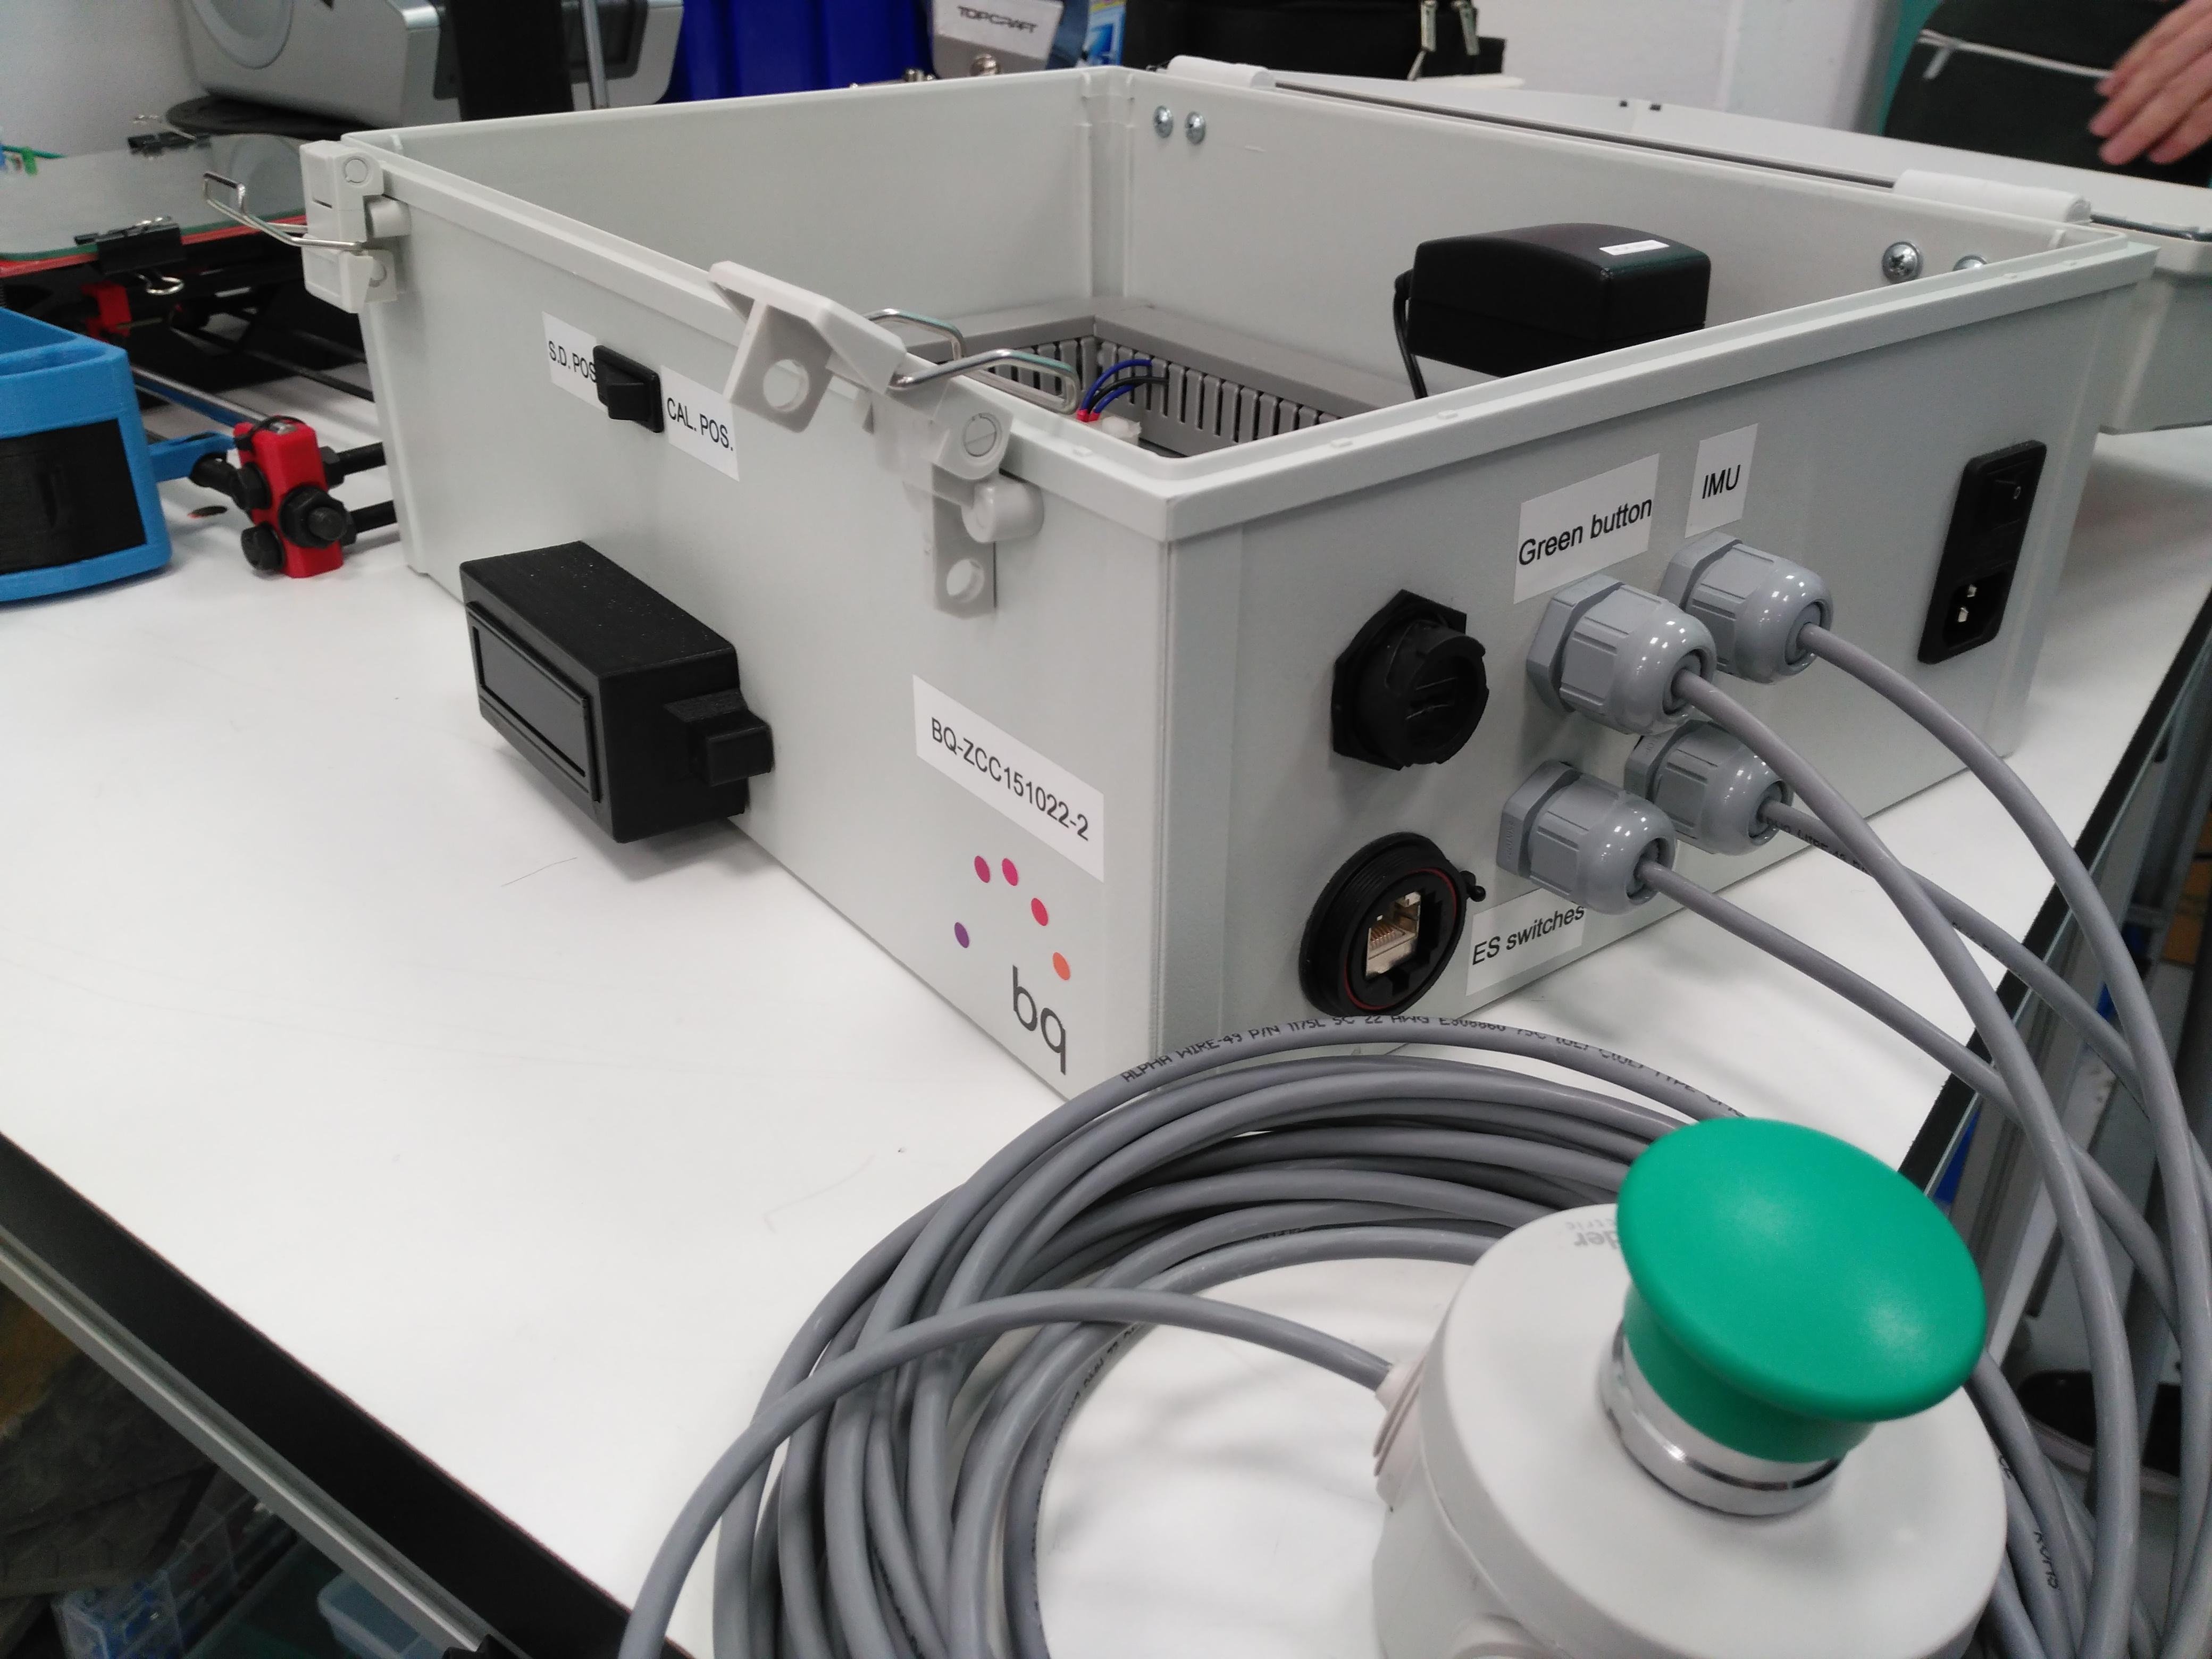
\includegraphics[width=120mm]{Figures/lateralArmario}
\caption{Armario final: Lateral}
\label{fig:lateralArmario}
\end{figure}

En el carril DIM se instala una toma de Schuko, al que se conectará la Raspberry PI para alimentar toda la electrónica. El armario es energizado por un conector a red eléctrica JR-101 con interruptor y fusible.

\begin{figure}
\centering
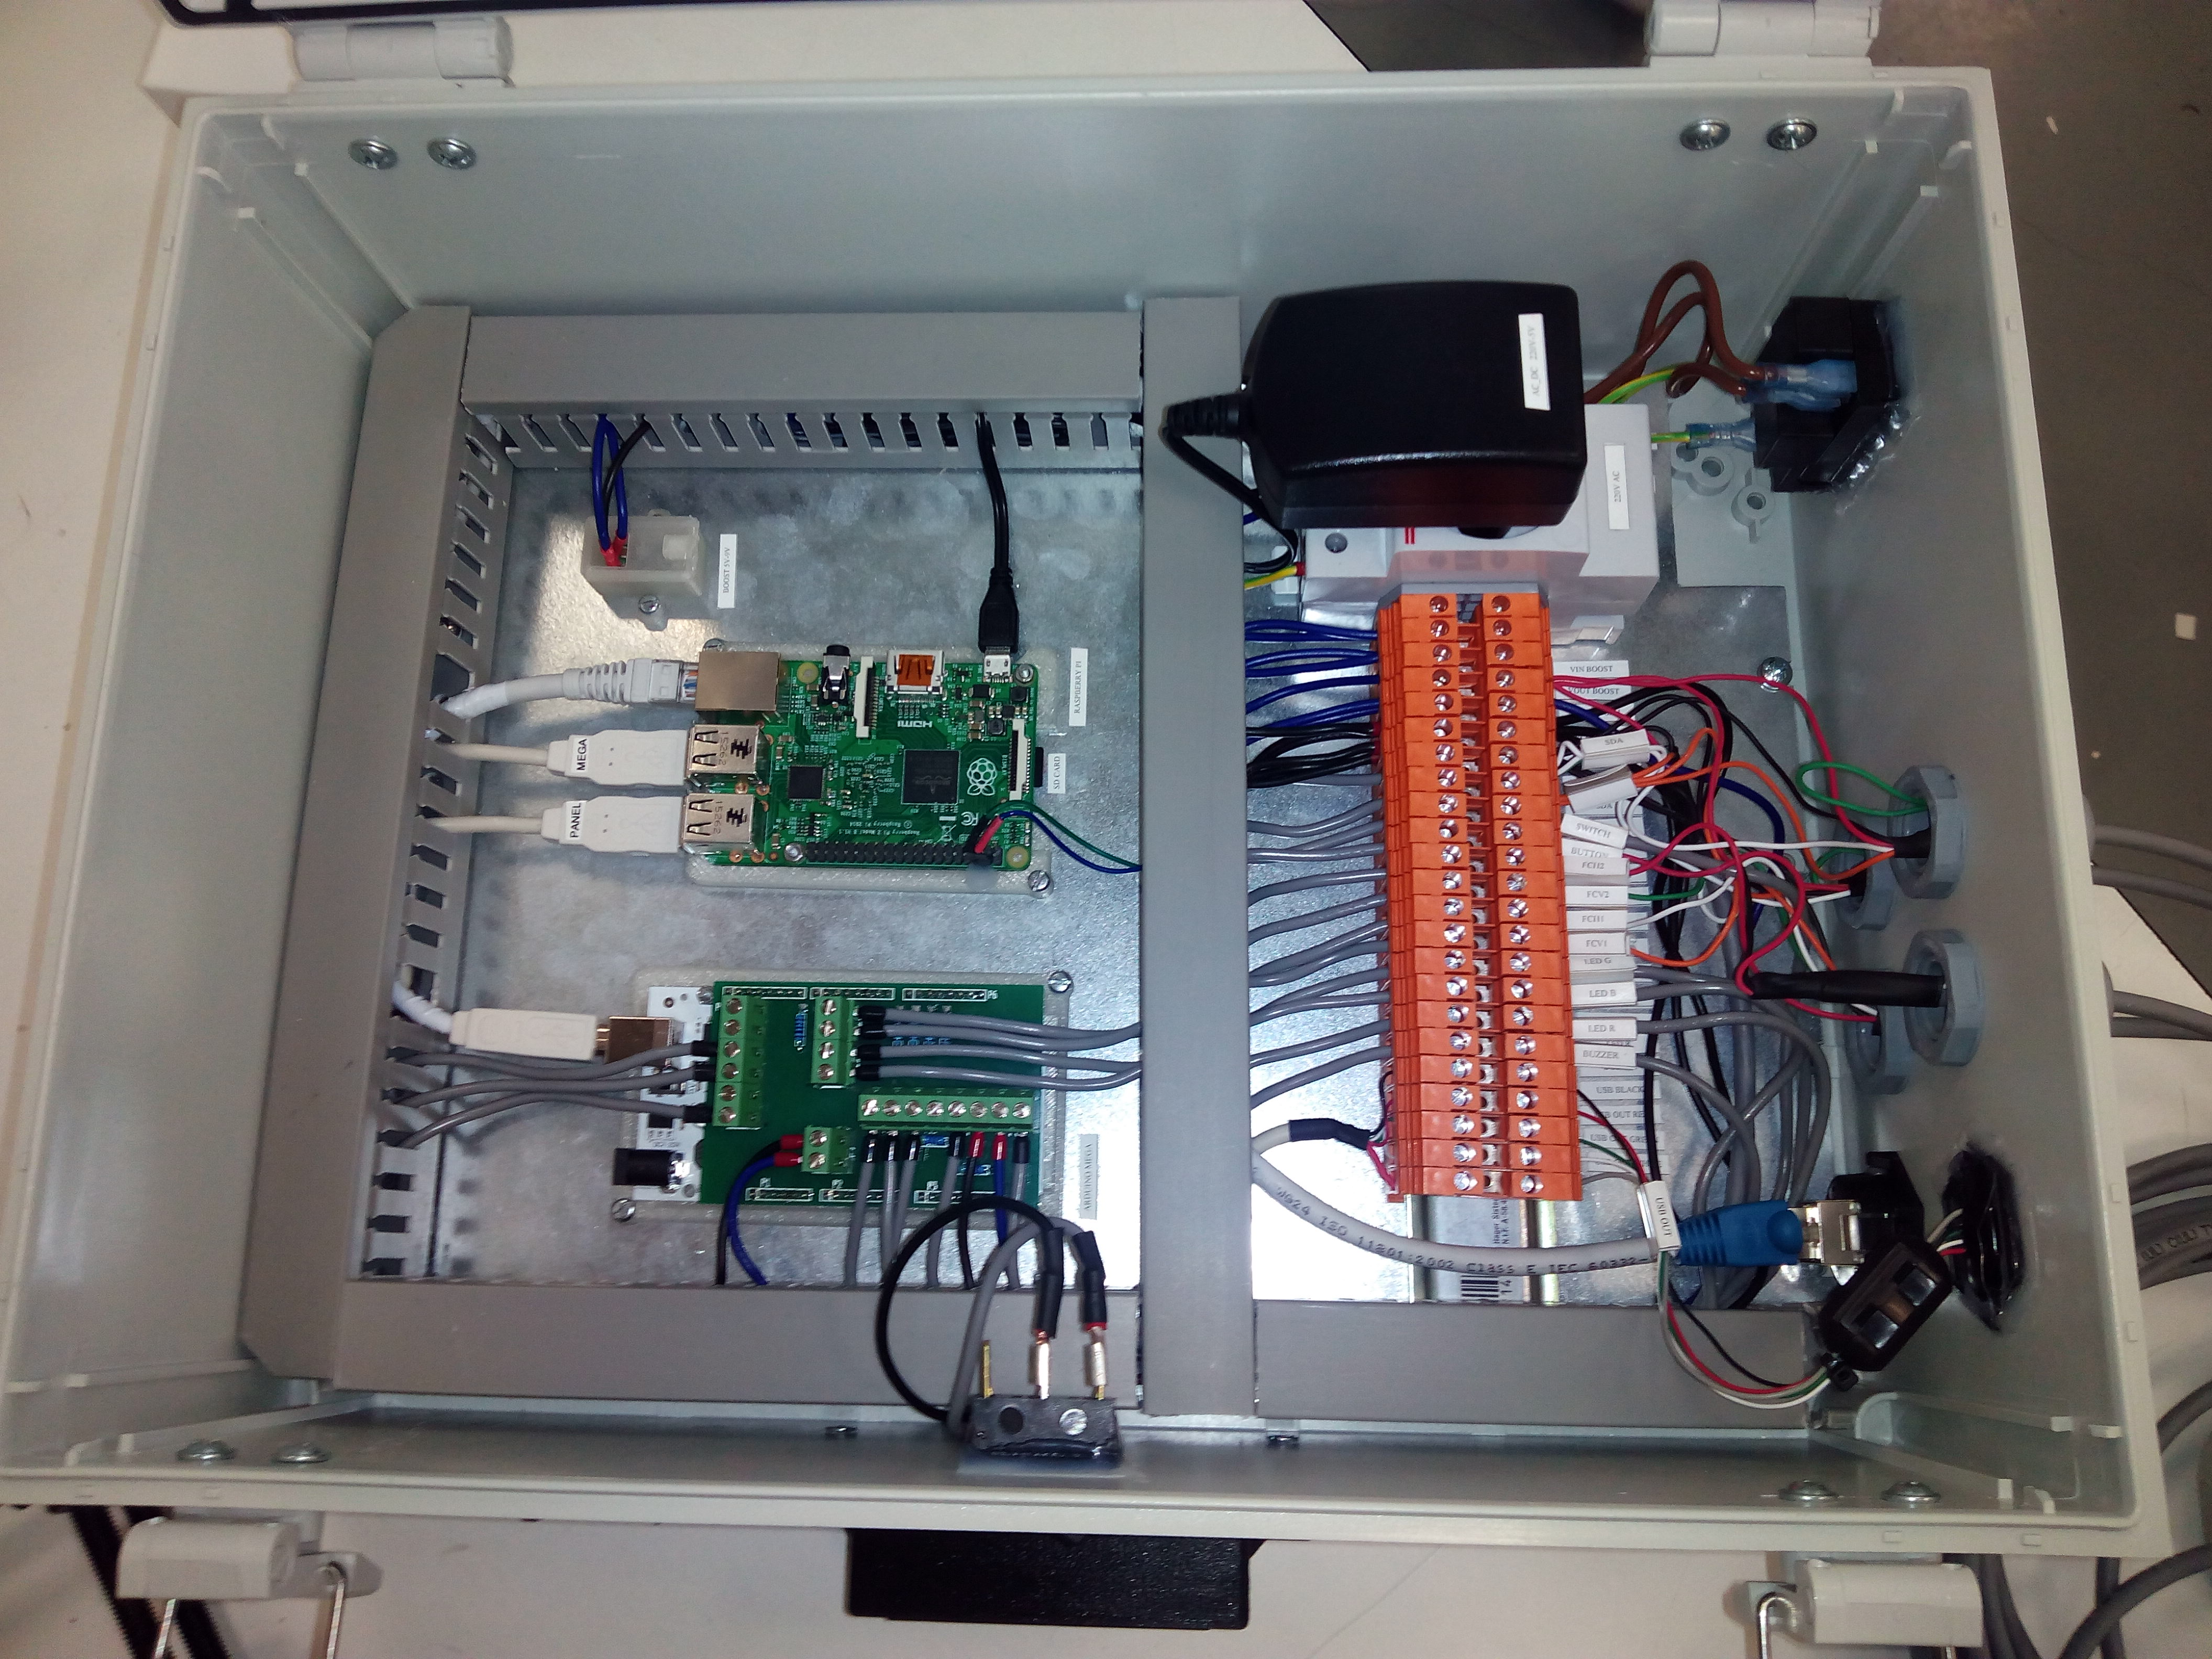
\includegraphics[width=120mm]{Figures/interiorArmario}
\caption{Armario final: Interior}
\label{fig:interiorArmario}
\end{figure}

Se pueden ver las Figuras \ref{fig:interiorArmario} y \ref{fig:lateralArmario}, interior y lateral del armario, respectivamente. Para detalle de las conexiones al clemero, se pueden consultar los planos eléctricos en el Anexo \ref{app:planosElectricos}.

\subsubsection{Mega}
Esta placa hace de cerebro del sistema a pesar de ser alimentada a través de la Raspberry, y de comunicar a través de ella con Zowi. Se pueden consultar las especificaciones en el Anexo \ref{app:mega-specs}.

\begin{figure}
\centering
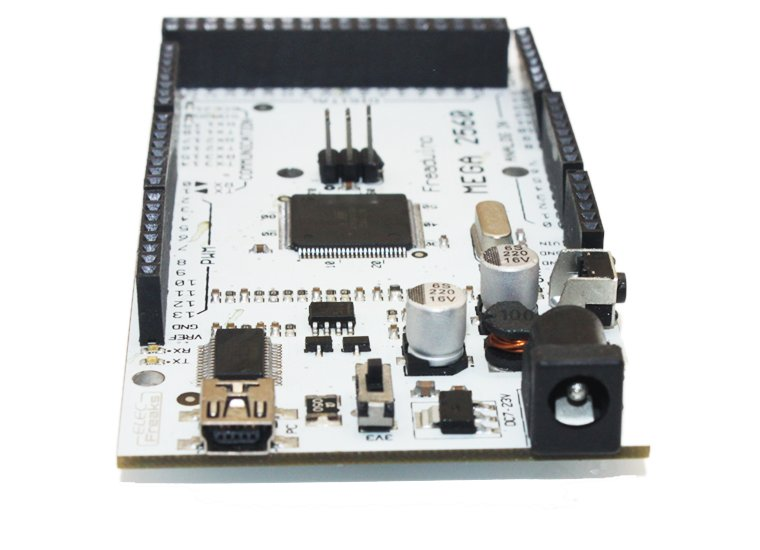
\includegraphics[width=105mm]{Figures/arduinoMega}
\caption{Freaduino Mega2560}
\label{fig:arduinoMega}
\end{figure}

Recibe las lecturas de los sensores IMU, tiene conectados los finales de carrera, interruptor, pulsador, panel LCD, buzzer y leds. Todas las conexiones cableadas de entrada/salida, así como la alimentación pasan por un shield diseñado para ésta aplicación.

Define una máquina de estados que mueve al operador por todos los pasos de la calibración y controla a la raspberry mediante un protocolo de instrucciones implementado para este fin que usa como canal el puerto serie por USB, tambien empleado para hacer llegar instrucciones a la placa de Zowi.

Podemos decir que Mega es la encargada de interactuar con el exterior y, dentro de nuestro sistema, realiza las funciones de un PLC. Para ello se ha elegido cuidadosamente cómo conectar los diferentes componentes a sus entradas/salidas, en el Anexo \ref{app:pinoutMega} se puede consultar el pin-out de ésta placa:
\begin{itemize}
  \item Leds y buzzer necesitan PWM para poder configurar los sonidos/colores.
  \item Los pulsadores y finales de carrera se han conectado a entradas que tienen asociadas resistencias de pull-up, conectadas fácilmente por software.
  \item Se ha alimentado por Vin en lugar de por USB para poder alimentar a todos sus dispositivos.
\end{itemize}

Información sobre software en la Subsección \ref{subsec:Software}. Para conocer con detalle las conexiones se pueden consultar los documentos del Anexo \ref{app:planosElectricos}.

\subsubsection{Shield Mega}
Se emplea el diseño de la shield de la versión prototipo del armario. En este caso se mandan a fabricar las PCBs, ya que nuestra fresadora no dió unos resultados tan profesionales.

\begin{figure}
\centering
\begin{minipage}{.5\textwidth}
  \centering
  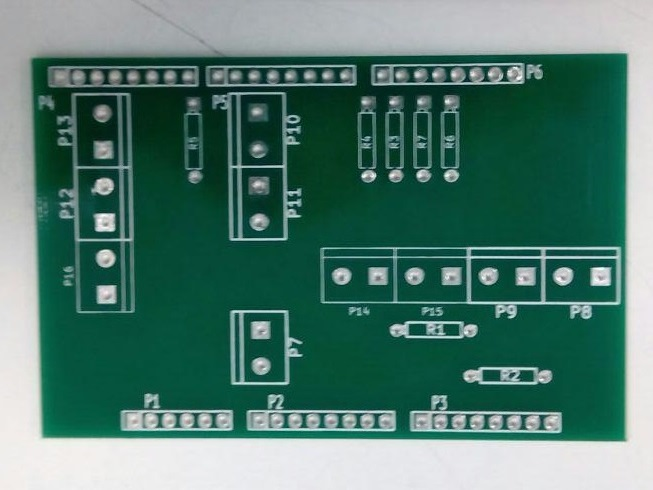
\includegraphics[width=.9\textwidth]{Figures/pcbMega}
  \captionof{figure}{PCB Shield}
  \label{fig:pcbdMega}
\end{minipage}%
\begin{minipage}{.5\textwidth}
  \centering
  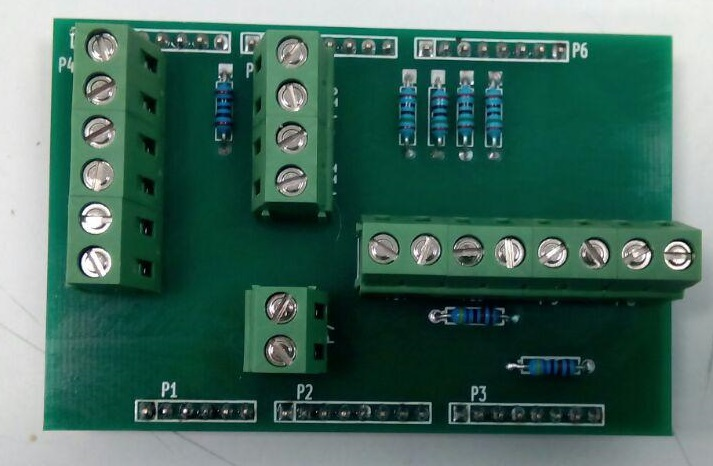
\includegraphics[width=.9\textwidth]{Figures/shieldMega}
  \captionof{figure}{Shield soldada}
  \label{fig:shieldMega}
\end{minipage}
\end{figure}

Esta shield es colocada sobre los pines de la Mega y nos proporciona unos borneros para facilitar la conexión cableada a los dispositivos de entrada y salida, así como a la alimentación.

Los esquemáticos y gerbers con el layout del diseño de la PCB se pueden consultar en el Anexo \ref{app:pcbFiles}. Para información más clara sobre conexiones, se pueden consultar los planos eléctricos de un armario, Anexo \ref{app:planosElectricos}.

\subsubsection{Raspberry PI 2}

Este ordenador (Figura \ref{fig:raspi}) aporta muchísimas mejoras de fácil implementación al sistema, además de su función principal, hacer de enlace entre Mega y la controladora de Zowi. Éstas mejoras serán definidas en la Subsección \ref{subsec:Software}, apartado dedicado al software. Se pueden consultar las especificaciones en el Anexo \ref{app:raspi-specs}.

\begin{figure}
\centering
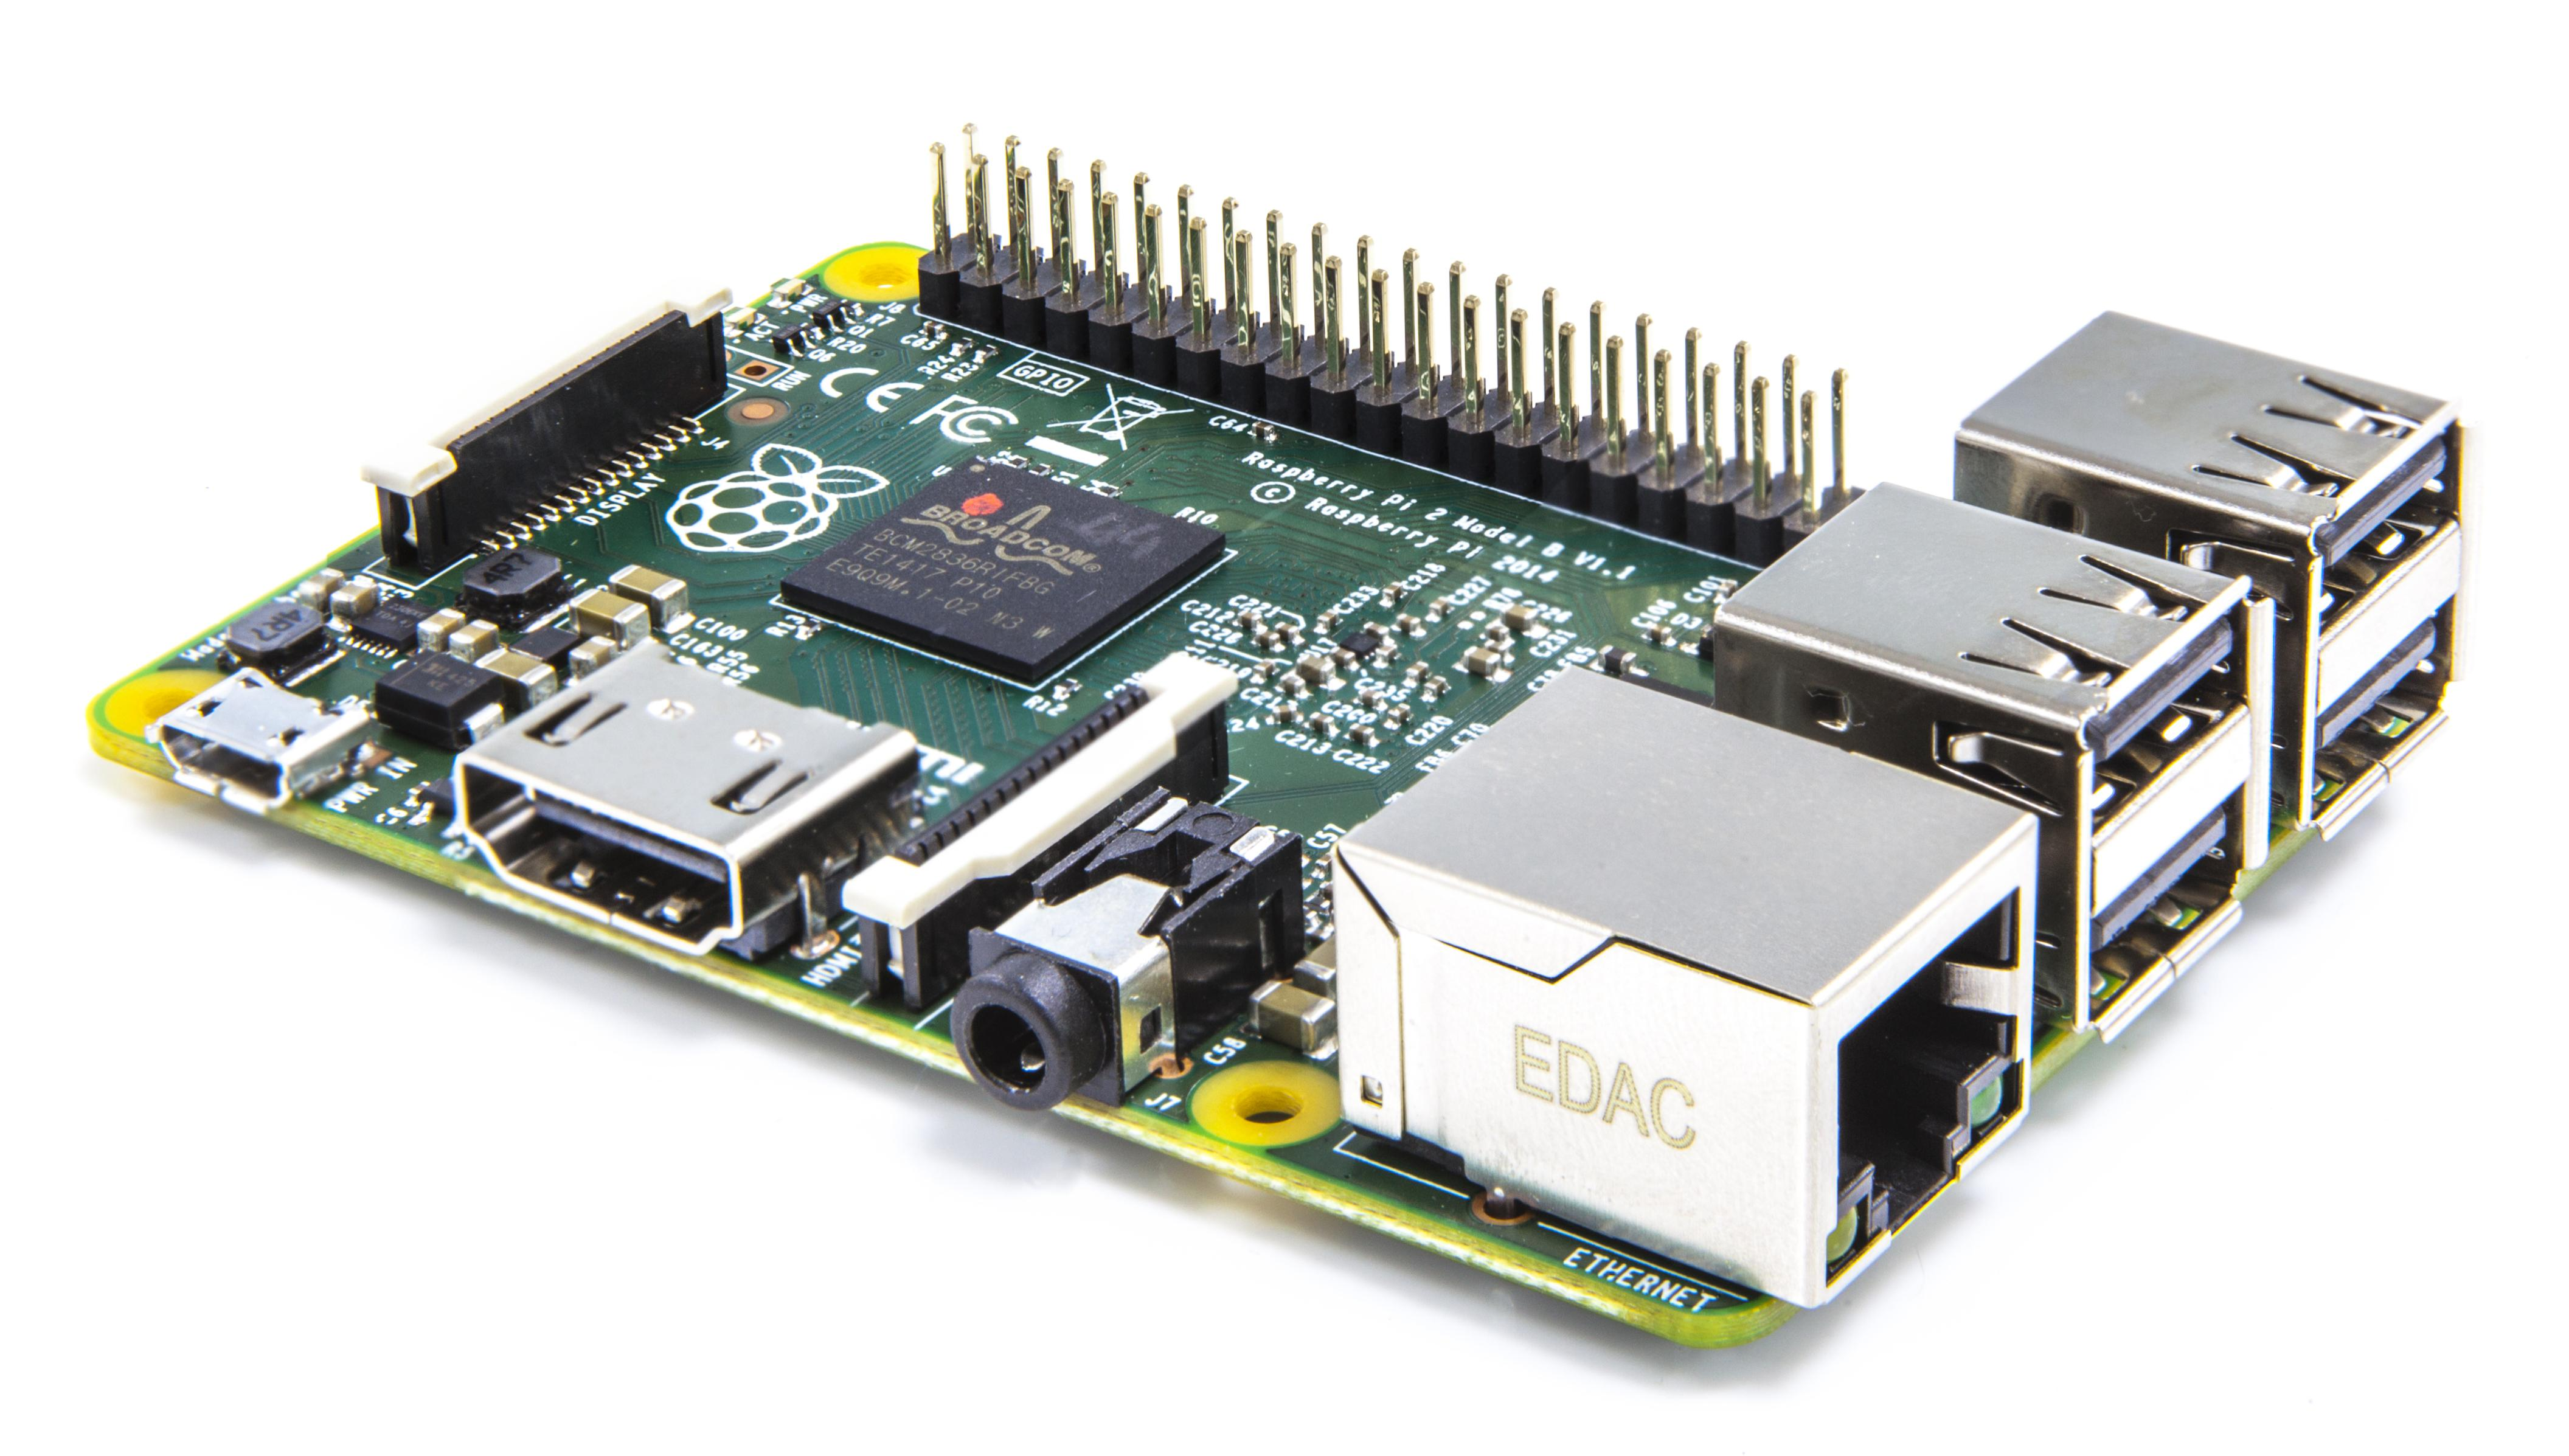
\includegraphics[width=100mm]{Figures/raspi}
\caption{Raspberry PI 2 - 1GB Ram}
\label{fig:raspi}
\end{figure}

Comunica con Mega y con las controladoras de los Zowi (Zum), para ello utiliza protocolo serie por cable USB con cada una de las placas. Además, por Ethernet, se puede acceder a ella por SSH (puerto 22) y por XRDP (puerto 3389) desde la misma red local o desde internet configurando propiamente el NAT; y una IP y puerto pueden ser configurados para guardar datos de calibración contra una base de datos remota.

Es alimentada por su toma microUSB, a través de un transformador conectado al Schuko del armario. Se encarga de alimentar y programar por USB a los Zowi, para lo que ha sido necesario desbloquear el límite de corriente suministrada por puerto USB por el sistema operativo (Se necesita suficiente potencia para mover los servos). También limenta a la Mega por su pin de 5V+, para lo que ha sido necesario elevar dicha tensión. Una vez más, se pueden ver los planos eléctricos para mayor detalle, Anexo \ref{app:planosElectricos} y Anexo \ref{app:planosEle2}.

\subsubsection{Power Boost}

La Mega debe ser alimentada a más de 7V. Para reducir número de transformadores y el espacio ocupado, se decide alimentarla a través de la raspberry.

\begin{figure}
\centering
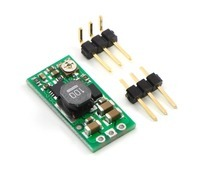
\includegraphics[width=70mm]{Figures/powerBoost}
\caption{Power Boost}
\label{fig:powerBoost}
\end{figure}

Este dispositivo (Figura \ref{fig:powerBoost}) acepta una tensión de entrada de 1.5V a 25V y, mediante el potenciómetro, permite ajustar su salida a valores entre 4V y 25V.

El power boost es ajustado para elevar la tensión suministrada por pines de la Raspberry de 5V a 9V para alimentar la Mega. Necesario para no tener que dar la corriente por el puerto USB. Aún desbloqueando el límite software de intensidad de la Raspberry, con lo que se consigue hasta 1.2A a 5V, el sistema no funciona correctamente al alimentar por USB ambas placas, Zowi carga su batería y mueve sus servos utilizando dicha corriente. De modo que se alimenta la Mega (y todo lo conectado a ella) desde el pin de 5v de Raspberry, sin usar el puerto USB y sin tener que introducir otro transformador en el armario.

\subsubsection{LCD Display}

Una pantalla es instalada para indicar al operador instrucciones e información sobre el uso del sistema. Se elige un display de 16 filas x 2 columnas y un backpack de Adafruit (Figura \ref{fig:backpack}) que nos permite comunicar con el display utilizando I\textsuperscript{2}C en lugar de una buena cantidad de salidas digitales, y que funciona con librerías más que probadas hechas por la comunidad.

\begin{figure}
\centering
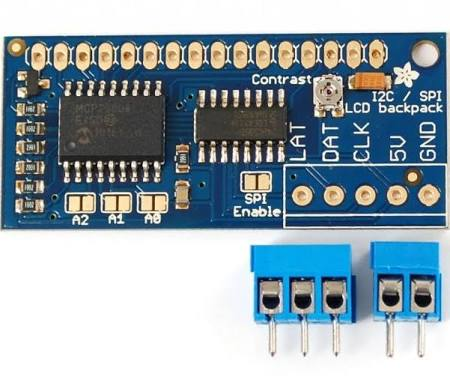
\includegraphics[width=75mm]{Figures/backpack}
\caption{Backpack para Display LCD}
\label{fig:backpack}
\end{figure}

\subsubsection{Otros componentes}

Además de los componentes principales comentados anteriormente, y de los sensores IMU tratados en el Marco Teórico (Capítulo \ref{Chapter2}), se emplean otros componentes menores como son los leds, el buzzer, los botones, finales de carrera, así como sus resistencias, ademas de las clemas, puntas, y más. En los planos eléctricos (Anexo \ref{app:planosElectricos}) y hoja de costes (Anexo \ref{app:BOM}), se puede consultar más información sobre su conexión o modelo.

\subsubsection{Zowi - Zum}

Como se ha comentado anteriormente, Zowi también forma parte del sistema. Su controladora tendrá conectados, entre otras cosas, los 4 servomotores responsables de mover las articulaciones. Comunica solamente con la Raspberry PI utilizando protocolo serie por cable USB. La Raspberry le descargará un software para poder interpretar las instrucciones recibidas, y ser capaz de mover los servos o guardar información en su EEPROM.

\subsubsection{Banco soporte Final de Zowi y zapatos}

Para validaciones y durante todo el desarrollo del proyecto -así como para su uso en Madrid, tras acabar la fase de producción en fábrica- se han empleado, y emplean, los diseños realizados por el autor, cuyas vistas se pueden consultar en el Anexo \ref{app:piezas}. No se especifican cotas de tolerancias por estar pensados para fabricar con impresoras 3D de filamento fundido, donde las dimensiones finales varían por parámetros como la temperatura o la velocidad de extrusión de la máquina.

\begin{figure}
\centering
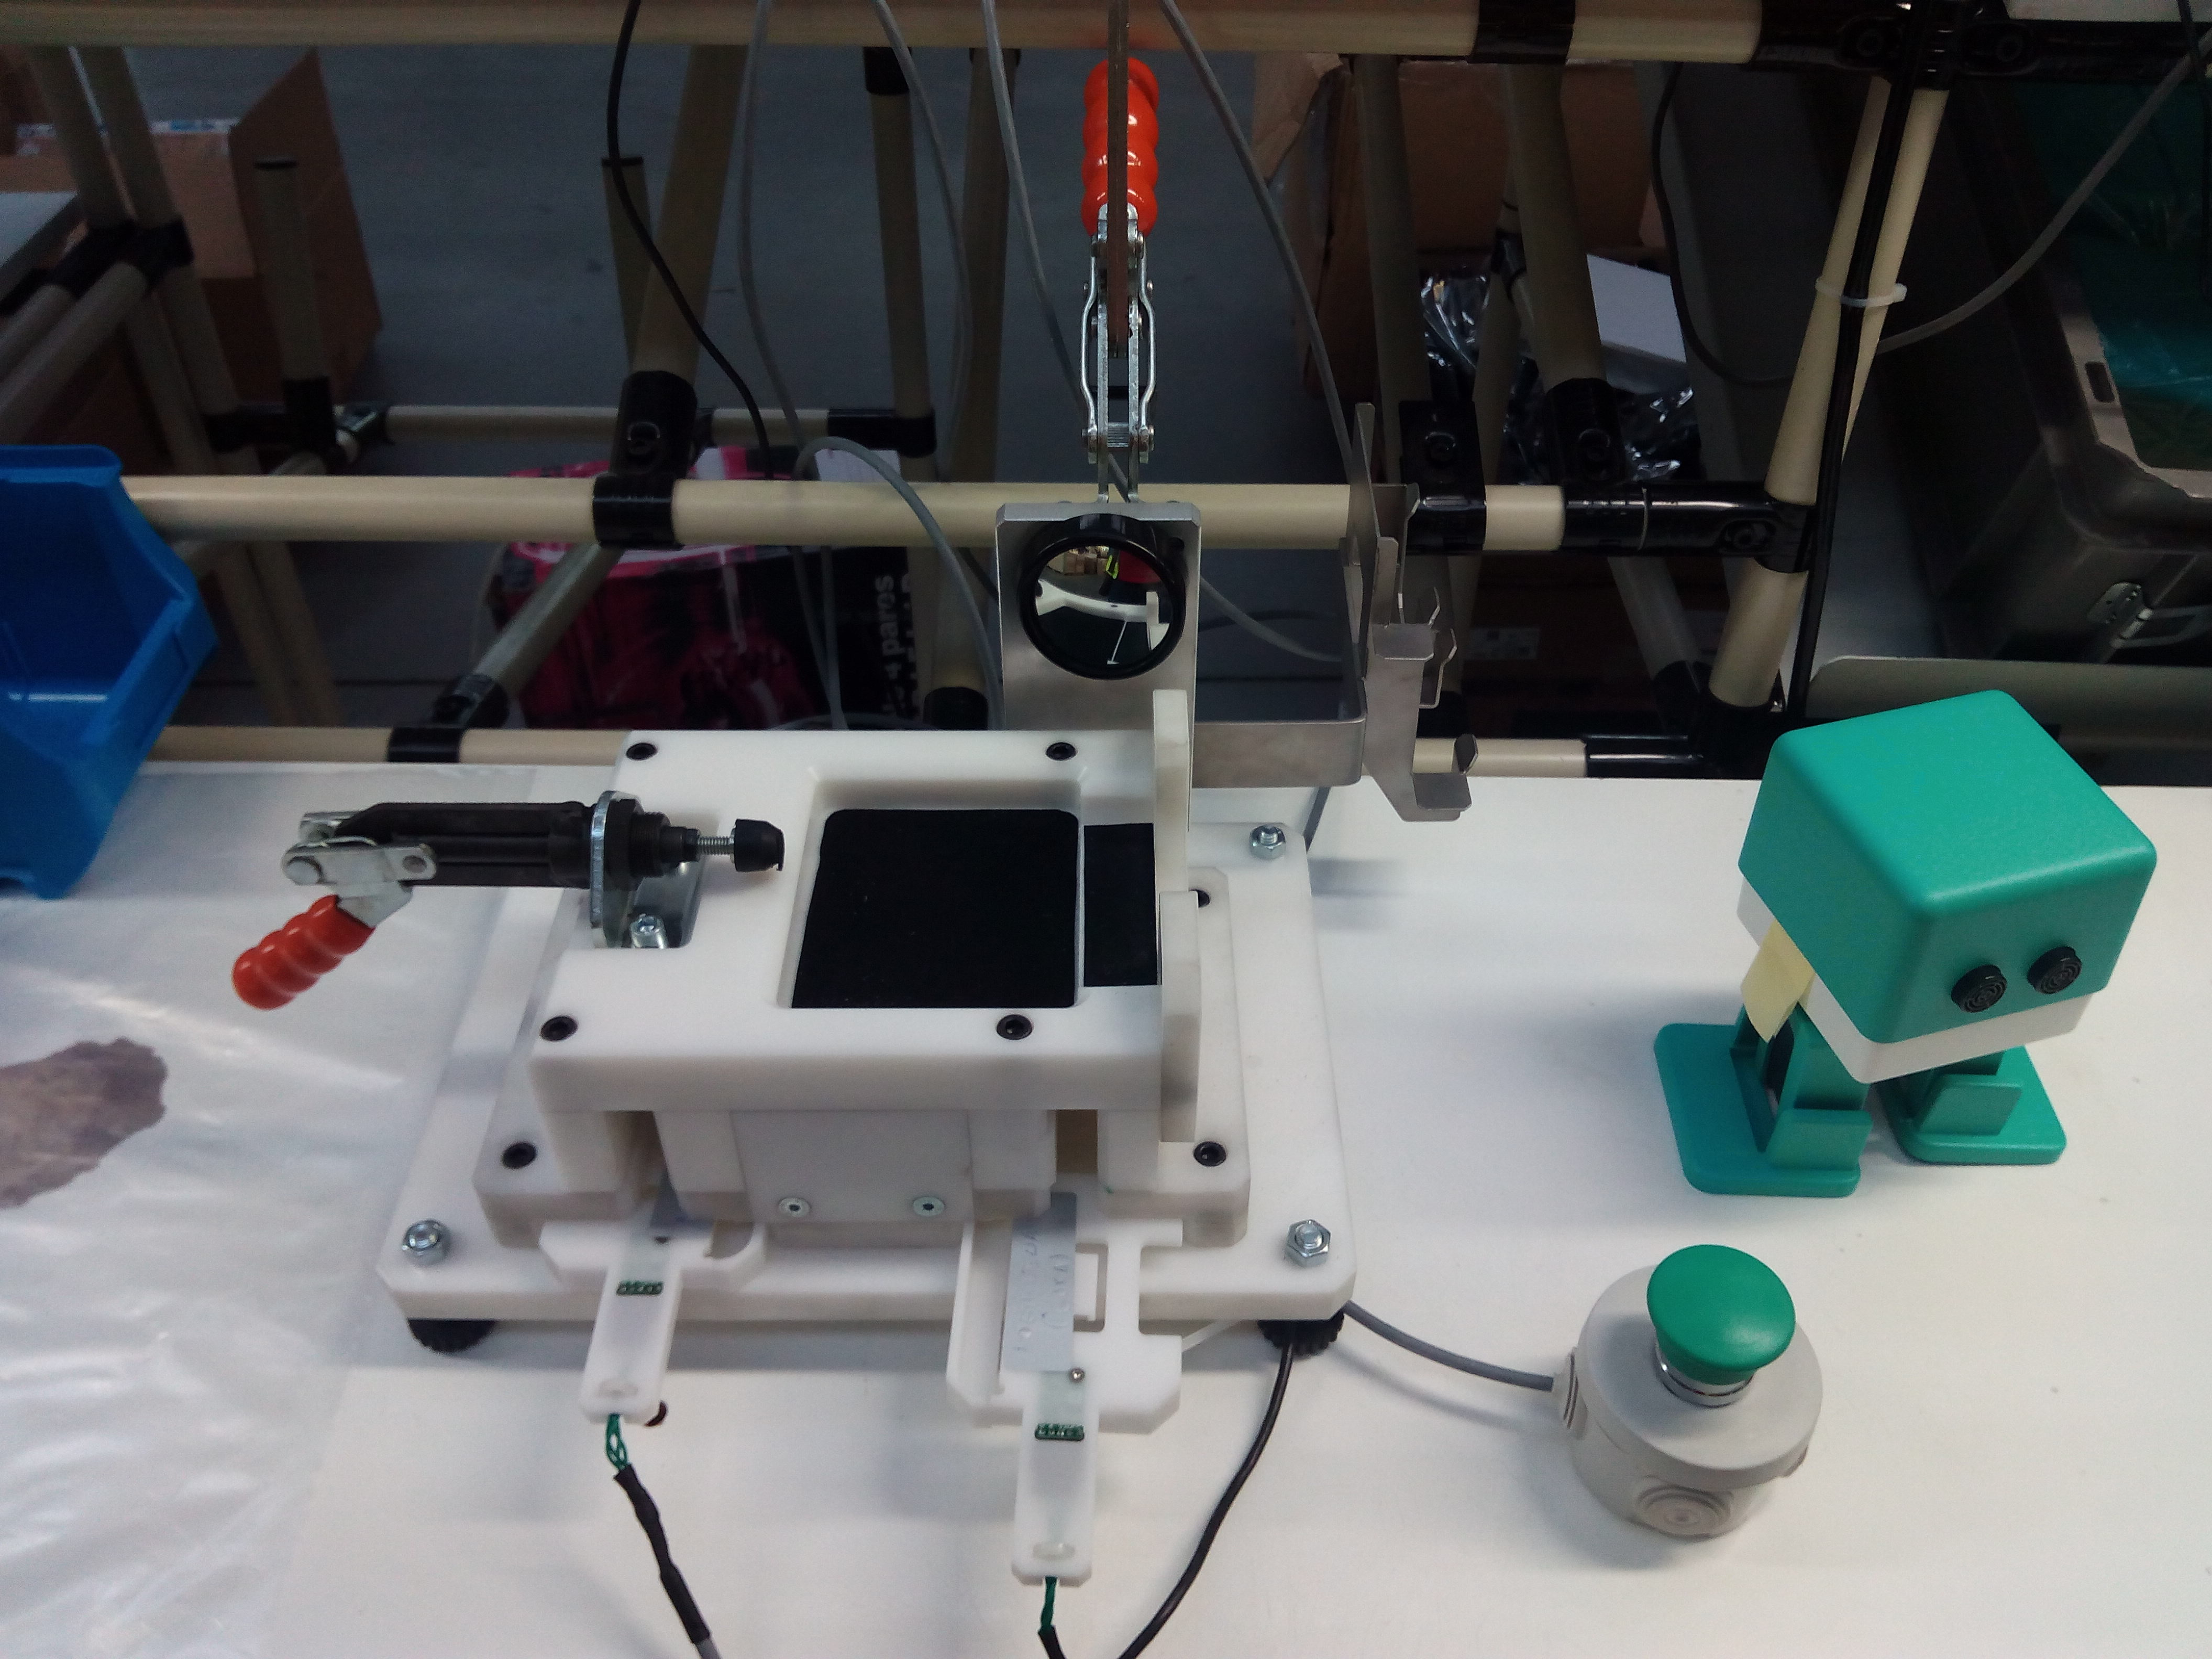
\includegraphics[width=120mm]{Figures/bancoFabrica}
\caption{Banco soporte y zapatos finales}
\label{fig:bancoFabrica}
\end{figure}

Sin embargo, el utillaje empleado en cadena de montaje (Figura \ref{fig:bancoFabrica}) fue rediseñado por el Dpto. de Mecánica y fabricado por sinterizado selectivo por láser, para lograr un acabado más preciso y mayor resistencia. Le añadieron palancas para fijar cada juguete y mejoraron los zapatos para facilitar la colocación.

%-----------------------------------
%	SUBSECTION 2
%-----------------------------------

\subsection{Software}
\label{subsec:Software}
En esta subsección se explicarán los aspectos relacionados con la programación del sistema y los algoritmos empleados. Se ha divido en tres partes, una para cada uno de los tres dispositivos principales, Mega, Raspberry y Zowi. Puede ser útil, para entender el funcionamiento del sistema, consultar los anexos \ref{app:usermanual}, \ref{app:pythoncode}, \ref{app:megacode} y \ref{app:zowicode}, donde se muestra el Manual de Usuario y el Código desarrollado.

\subsubsection{Mega}
Este dispositivo se puede programar utilizando el lenguaje de Arduino,  que es una adaptación de C++ que proveniene de avr-libc y provee de una librería de C de alta calidad para usar con GCC en los microcontroladores AVR de Atmel y muchas funciones específicas para los MCU AVR de Atmel. Su simplicidad y la implicación por parte de la comunidad hacen realmente fácil y rápido su uso y aprendizaje.

El programa principal ha sido creado en el entorno de Arduino, en un fichero (.ino). Se emplean las funciones de Arduino precocinadas y se extiende de librerías de Arduino, programadas en C++, para todo lo posible, a destacar:
\begin{itemize}
  \item LiquidCrystal para escribir al display LCD.
  \item Wire para la comunicación  I\textsuperscript{2}C.
  \item Ficheros de la librería MinIMU, que extiende a su vez de las librerías del giróscopo y el acelerómetro, L3G.h y LSM303.h, respectivamente.
\end{itemize}

El programa de Mega sigue una estructura de máquina de estados que se encarga de llevar al operador por los diferentes pasos del proceso de calibración, es aquí dónde se toman las lecturas de las posiciones de los servos y se decide cuánto se han de mover, dónde se valida el resultado de la calibración y dónde se produce la interacción entre la máquina y el usuario. Se puede decir que es el principal dispositivo del sistema.

Para conocer la lógica de la máquina de estados, se pueden consultar los diagramas del Anexo \ref{app:megadiag}, para conocer el proceso de uso, como operador, se puede consultar el manual de usuario del Anexo \ref{app:usermanual}.

\paragraph{Protocolo de comunicación}

Para lograr enviar instrucciones a la controladora del robot utiliza como intermediario a la Raspberry, que establece una comunicación serie por USB con ambas controladoras. Se desarrolla un protocolo de instrucciones que tiene las siguientes partes:

\begin{itemize}
  \item Signo de dólar (\$) como carácter inicial de la trama.
  \item 4 caracteres que indican el comando función en cuestión.
  \item Dos puntos (:) para indicar inicio de valores de parámetros.
  \item Parámetros de la función, si los tuviera, separados por el carácter (*).
\end{itemize}

Instrucciones desde Mega:

\begin{itemize}
  \item \textbf{IZUM:} Comando que indica a Raspberry que cargue el programa calibración en Zowi.
  \item \textbf{ROFC:} Comando leer offset de las articulaciones de Zowi.
  \item \textbf{WOFC:} Ordena a Zowi escribir los valores de offset en su EEPROM. Se envía con la instrucción un número (1 o 2) para indicar pierna derecha/izquierda, además del separador (*) y las posiciones en grados, 3 dígitos cada una, separadas por el asterisco (*).
  \item \textbf{M90C:} Ordena a Zowi mover todos los servos a la posición 90º, utilizando la librería servo.
  \item \textbf{MHOC:} Ordena a Zowi mover todos los servos a la posición 90º con la corrección guardada en la EEPROM, si la hay.
  \item \textbf{MHOC:} Ordena a Zowi mover todos los servos a la posición indicada, necesita como parámetro un número de tres cifras que indique la posición en grados.
  \item \textbf{MSxC:} Comando a Zowi para mover el servo indicado a la posición indicada. Necesita un número del 1 al 4 que indica el servo a mover, el separador (*), además de 3 dígitos que indiquen el grado.
  \item \textbf{WERC:} Comando que envía los errores medidos tras la calibración a Raspberry. Para cada servo se envía el error con 3 dígitos enteros más 2 decimales, separados por punto. Los datos de cada servo están separados por (*).
  \item \textbf{FZUM:} Ordena a Raspberry que cargue el programa final en Zowi.
  \item \textbf{ROFF:} Comando a Raspberry para apagar el sistema (Shut down).
  \item \textbf{WSQL:} Ordena Raspberry que cierre comunicación con Zowi y registre una entrada de fin de calibración en la base de datos.
\end{itemize}

Si bien las instrucciones anteriores fueron útiles durante el desarrollo, se acabó utilizando, principalmente, el movimiento de un solo servo por ser más controlado, se observaron algunos funcionamientos no deseados al tener en movimiento los 4 servos simultáneamente, además de la batería en carga.

Como entrada, Mega recibirá 'M' o 'B' desde Raspberry en los estados que requieren feedback para determinar el siguiente paso en la máquina de estados, indicando estos 'Mal' y 'Bien', respectivamente. Las funciones de lectura como ROFC tambien resultaron útiles durante el desarrollo, sin embargo no se utilizan en la versión final.

\paragraph{Configuración}

Mega permite hasta 3 canales adicionales de comunicación serie, Serial1 utiliza los pines 19 como RX y 18 como TX para una comunicación serie TTL a 9600 baudios. Gracias a un cable TTL-USB, es posible debugear y desarrollar fácilmente, aún teniendo utilizado el puerto serie habitual para comunicar con Raspberry.

Programación para los componentes acústicos y luminosos utilizando las librerías stándar de Arduino, que permiten emitir un sonido o establecer el color de una luz con una simple línea de código, también se recurre al uso de las resistencias de pull-up integradas, activadas en la declaración del tipo de pin, para reducir la cantidad de electrónica necesaria para los finales de carrera y pulsadores.

\paragraph{Algoritmo básico de calibración}

Este algoritmo se ejecuta para la correcta calibración de cada uno de los juguetes.

Inicialmente se mandan los servos del robot Zowi a las posiciones correspondientes a 90º, se recuerda que el rango del servo es 0-180º, y que el juguete necesita un rango de solamente unos 80º.

La calibración consiste en tomar la lectura de los sensores IMU, de cada sensor interesan 2 orientaciones, una de ellas directamente relacionada con la posición de la cadera del robot, y la otra con el pié. Leyendo ambos sensores se obtienen las 4 posiciones de los servos.

Se calcula el desfase entre la posición leída y la posición actual según el programa de Zowi (inicialmente 90º), y se calcula la nueva posición necesaria a establecer en el servo para obtener los 90º deseados.

El proceso de lectura-corrección se lleva a cabo de forma iterativa hasta obtener una lectura con error inferior a 1º respecto a 90º.

\paragraph{Calibración de los sensores}

Esta calibración se ha de realizar cada vez que el sistema es iniciado o reiniciado.

Mediante las funciones de la librería de MinIMU, se establecen los ángulos cero para cada eje, para ello el operario es guiado a insertar los zapatos (que contienen los sensores) en los cajetines del banco de calibración, en éste paso se toman medidas hasta valorar que la calibración ha sido correcta. En esta etapa se corrigen pequeñas inclinaciones que pueda haber en el espacio de trabajo. Es la parte más crítica del proceso, porque la calibración se ve muy afectada por el movimiento, vibraciones o incluso campos magnéticos.

Durante el algoritmo de calibración se ha hablado del ángulo de 90º como ángulo deseado. Realmente, el valor éste ángulo para las caderas se corresponde con el 0º, mientras que para los piés se corresponde con el 90º, por lo que tambien es ajustado en esta etapa. Tras valorar que los ángulos 0º han sido bien definidos y su lectura es estable, se ha de girar cada zapato 90º utilizando los cajetines verticales. En esta fase se corregirá el pequeño error que pueda tener el sensor en esos 90º (no suele ser mayor de 1º).

\paragraph{Calibración del acelerómetro}

Configuración necesaria cada vez que se reemplace el sensor. Ésta es la única configuración necesaria para replicar el sistema.

Esta calibración no forma parte del programa del sistema, sino de su configuración e instalación. En los 2 armarios que se han creado, se utilizan en total 4 sensores IMUs, los circuitos integrados que contiene no son exactamente iguales y, por recomendación del fabricante y creador de la librería de MinIMU, se han de ajustar los valores máximos y minímos crudos del magnetómetro (mismo encapsulado que el acelerómetro). Para ello se utiliza un programa del fabricante que muestra, por el puerto serie, el valor máximo y mínimo crudos registrados mientras el sensor es movido en todos los ángulos. Estas constantes son introducidas en el programa de cada armario para ser utilizadas por la librería del acelerómetro, LSM303.

\subsubsection{Zowi}

El programa definido para la controladora de Zowi es un intérprete de los comandos definidos. La Raspberry descargará dicho intérprete en el microcontrolador de Zowi para poder comunicarle las posiciones a las que ha de mover los servos, y los valores de calibración que tendrá que guardar en su memoria EEPROM, memoria que no es sobrescrita en el proceso de programación habitual de la placa controladora.

Adicionalmente, la controladora de Zowi cuenta con un módulo de EEPROM por  I\textsuperscript{2}C, donde se recogen datos de fabricación de la placa. De esta forma se tienen 2 módulos de EEPROM, dejando el módulo del microcontrolador disponible para ser modificado por los usuarios de la placa.

Es en el módulo habitual donde se registran los valores de calibración del servo, pudiendo ser configurados por los usuarios en caso de que desmonten el juguete o reemplacen algún componente. Por otro lado, desde el módulo EEPROM por  I\textsuperscript{2}C, se obtendrá el número de serie, que almacenará la Raspberry en la base de datos con fines de trazabilidad.

Las librerías que se utilizan serán I2C\_eeprom.h y las estándar Servo.h para el movimiento de los servos y EEPROM.h para guardar los valores de calibración.

\paragraph{Protocolo visto desde Zowi}

Las siguientes instrucciones son recibidas por Zowi en la última versión del intérprete:

\begin{itemize}
  \item \textbf{MSxC:} Al recibir este comando, Zowi mueve el servo indicado a la posición indicada. El primer parámetro es un número del 1 al 4 que indica el servo a mover, seguido del separador (*) y 3 dígitos que indican el grado.
  \item \textbf{WOFC:} Zowi calcula el valor de offset a partir de las posiciones recibidas y los escribe en su EEPROM. Las instrucciones contienen un número (1 o 2) para indicar pierna derecha/izquierda, además del separador (*) y las posiciones en grados, 3 dígitos cada una, separadas por el asterisco (*).
  \item \textbf{M90C:} Zowi mueve todos los servos a la posición 90º por defecto.
  \item \textbf{MHOC:} Zowi lee el valor del offset de las articulaciones en su EEPROM y mueve todos los servos a la posición 90º con la corrección.
\end{itemize}

Se implementa una instrucción de salida, utilizando el mismo protocolo que se ha visto en Mega (instrucción delimitada por "\$" y "\#"), Zowi lee el número de serie de su controladora (6 dígitos) y se lo envía a la Raspberry con la instrucción \textbf{OKNS:}.

\subsubsection{Raspberry}

La Raspberry resulta ser un componente tan importante como la Mega dentro del sistema. Inicialmente fue incluída para hacer de nexo en la comunicación entre ambos controladores (Mega y ZUM de Zowi), pero inmediatamente se implementaron algunas funcionalidades adicionales.

Este ordenador tiene instalado un sistema operativo Raspbian, versión adaptada de Debian a Raspberry, concretamente se usa la última versión estable en el momento de desarrollo, Wheezie.

El lenguaje elegido para hacer el software es python, por lo rápido que resulta desarrollar con éste lenguaje y por ser el más familiar para el autor. Se instalan por tanto los paquetes necesarios (el entorno python-dev, el gestor de paquetes PIP y el gestor de entornos virtuales, virtualenv). Las librerías empleadas son serial para las comunicaciones serie, os para poder ejecutar comandos del sistema operativo y pymysql para poder escribir en bases de datos MySQL.

Para que el controlador de Zowi interprete las instrucciones que recibirá, se ha de descargar el intérprete creado. Esto requiere que Raspberry programe el micro ATMega328p de Zowi, para ello se utiliza la herramienta AVRdude como instrucción del sistema operativo, directamente desde el programa corriendo en python.
El programa en Arduino del intérprete está convertido en un fichero hexadecimal ya compilado con el entorno de Arduino, AVRdude escribirá este programa en el microcontrolador de Zowi.

Al arrancar el sistema operativo y la script, se inicia comunicación con Mega usando el puerto ttyUSB0 y envía un “1” para inicializar el programa. La Raspberry permanecerá a la escucha, los dispositivos conectados (Mega -y Zowis tras la descarga del intérprete-) envían instrucciones utilizando el protocolo implementado ya comentado en los apartados anteriores, cualquier instrucción a Raspberry irá contenida entre “\$ … \#”. Las instrucciones de Mega que han llegar a Zowi, se envían ya sin los delimitadores (\$ y \#), es decir, solamente el contenido de la instrucción.

Además de delimitar fácilmente qué datos son instrucciones, nos permite poder hacer eco del resto de datos recibidos por serie, para debug o información de los programas de las Arduino en Raspberry.

\paragraph{Máquina de estados en Raspberry}

Se muestra la respuesta de la script de python a las diferentes instrucciones recibidas:

\textbf{IZUM:}
Cuando se recibe este código, Raspberry programará la ZUM de Zowi con el software de calibración (el intérprete), ubicado en el siguiente directorio:
\begin{center} /home/pi/zowi/python/zowi\_offset\_i2c.cpp.hex \end{center}

El programa es subido usando la instrucción de AVRdude:
\begin{center} avrdude -patmega328p -carduino -P/dev/ttyUSB1 -b 115200 -D -Uflash:w:/home/pi/zowi/python/zowi\_offset\_i2c.cpp.hex:i \end{center}

Como se ha dicho anteriormente, éste programa es necesario para interpretar los códigos e instrucciones enviados desde Mega. Se envía un código de confirmación con el texto “M” o “B” indicando a Mega indicando el resultado del proceso.

\textbf{FZUM:}
Cuando se recibe este código, se programa ZUM de Zowi con el programa final del juguete. El fichero está está en el siguiente directorio:
\begin{center} /home/pi/zowi/python/ZOWI\_BASE\_v0.cpp.hex \end{center}

Se envía un código de confirmación con el texto “M” o “B” indicando a Mega indicando el resultado del proceso.

\textbf{ROFF:}
Indica que el sistema se debe apagar, cuando se recibe este comando desde Mega, se apaga el sistema operativo.

\textbf{WERC:}
Este código indica los errores de calibración de cada articulación, es decir, cuántos grados de diferencia se han conseguido entre los valores teóricos y los medidos tras finalizar una calibración, sea exitosa o fallida. Se almacenan dichos valores para ser guardados, posteriormente, en la base de datos.

\textbf{MSxC:}
El resto de instrucciones de movimiento de servos ya comentadas en los apartados de software de Mega y Zowi, se envían directamente de Mega a Zowi. Para el caso de movimiento de un servo específico, \textbf{MSxC}, se almacenan los últimos valores enviados, para poder ser volcados a la base de datos cuando se reciba la instrucción adecuada.

\textbf{WOFC:}
Este código es enviado indicando las nuevas posiciones de los servos de Zowi, las posiciones que hacen que sus articulaciones estén alineadas y calibradas. Raspberry envía estos valores a Zowi para que éste calcule los desfases y los escriba en su memoria EEPROM.

\textbf{OKNS:}
Es la única instrucción que proviene de Zowi, e indica el número de serie de la placa controladora del ejemplar, Raspberry almacena dicho número para su escritura en base de datos.

\paragraph{Base de datos}

Se instala en el sistema una base de datos MySQL local, contra la que se registran los eventos que suceden durante el uso del sistema. Además, la script del programa principal de python está también preparada para escribir a una base de datos remota.
Se escribe en la base de datos tras cada calibración, sea buena o mala. Para lo que se utiliza un campo de "Estado" que valdrá 1 o 0, respectivamente.
Se registran los errores de calibración leídos en Arduino Mega para cada uno de los 4 servos.
Se registran además las 4 posiciones "trim" de los servos, las mismas que se hacen llegar a la placa de Zowi para que guarde en su EEPROM para salir a venta.
Se registra la hora, con fines estadísticos de tiempos y tambien el número de serie del Zowi conectado con fin de trazabilidad en caso de errores/reclamaciones.

Cuando se inicia o apaga el sistema, se escriben todos los campos a 1 salvo la hora para el caso de inicio. Y todos los valores a 0 salvo la hora para el fin.

Durante el uso de los primeros días en producción surgieron algunos problemas, para los que se definieron unos códigos de error y se implementaron ciertas correcciones de forma remota, de la misma forma que para inicio y final se usan valores a 1 y a 0, para estos errores utilizamos:

\begin{itemize}
  \item \textbf{Valores a 2:} Excepción del cable, producido por pérdida de comunicación con Mega.
  \item \textbf{Valores a 3:} Otros errores no conocidos, por excepción en el programa principal.
  \item \textbf{Valores a 4:} Error conexión fallida al intentar descargar intérprete a Zowi.
  \item \textbf{Valores a 5:} Error conexión fallida al intentar descargar programa final a Zowi.
\end{itemize}

Para ver la estructura de la tabla, se puede consultar el Anexo \ref{app:dbsctruct}.

\paragraph{Configuración adicional}
El servicio de escritorio remoto XRDP es instalado, lo que nos permite utilizar la interfaz gráfica de forma remota.

El entorno de Arduino es también instalado, permitiendo modificar el programa de Mega desde Raspberry. Se instalan también las librerías empleadas en los programas creados. El entorno de Arduino instalará AVRdude para realizar la programación de los microcontroladores.

En el fichero de configuración de Raspberry \textbf{/boot/config.txt} se configura \textit{max-usb-current=1} lo que nos permite suministrar hasta to 1.2A por USB para alimentar a Zowi (por defecto, límitado a 600mA).

Se configura el Login automático mediante el fichero \textbf{/etc/inittab}. De este modo el sistema funciona como servidor en lugar de esperar que un usuario introduzca sus credenciales. Procedimiento en el Anexo \ref{app:autologin}.

Se crea una una script, \textbf{running.sh} que funciona como monitor, hará que la script principal sea arrancada siempre que no esté corriendo. Esta medida rearma el sistema ante algunos errores, como por ejemplo, intentar programar una placa que deja de estar energizada o es apagada o desconectada durante la programación. Anexo \ref{app:running}.

Se configura el arranque automático de la script anterior al encender el sistema, dicha script levantará el programa principal nada más ser iniciado el sistema. El arranque automático se logra mediante el fichero \textbf{ZowiInit}, que se puede consultar en el Anexo \ref{app:zowiinit}.

Durante el desarrollo se creó un documento de notas para facilitar la reproducción de la instalación desde cero, además de la creación de unas imágenes completas de la tarjeta SD de la Raspberry, utilizando Win32DiskImager. Se anexan las mencionadas notas por si pudiesen resultar de interés para el lector, Anexo \ref{app:raspi-tips}.

Tras observar el funcionamiento del sistema en producción durante algunos días, se detectan algunos errores al conectar y desconectar repetidas veces los robots. El sistema podría no funcionar si se asigna un puerto diferente a Mega, o si se inicia el sistema con un Zowi ya conectado. Para mejorar ésto, se crean unas reglas (fichero \textbf{50-usbportsbq.rules}) para definir el puerto según el ID del fabricante de la placa, asignando a cualquier puerto USB conectado a Raspberry el alias de “mega” o “zowi” en lugar de ttyUSBX, nombre por defecto) . Dichas reglas son instaladas dentro de \textbf{/etc/udev/rules.d/}. El programa de python es modificado para asumir estos cambios. Las notas sobre el fichero de las reglas se puede ver en el Anexo \ref{app:rules}. Además, se implementa una nueva función en el código que desconecta y conecta eléctricamente la bahía del puerto USB de Zowi por software (utilizando \textbf{bind} y \textbf{unbind}) antes de cada programación. Los errores y reinicios se reducen inmediatamente.

% Chapter Template

\chapter{Conclusiones y trabajos futuros} % Main chapter title

\label{Chapter4} % Change X to a consecutive number; for referencing this chapter elsewhere, use \ref{ChapterX}

%----------------------------------------------------------------------------------------
%	SECTION 1
%----------------------------------------------------------------------------------------

\section{Conclusiones}

El sistema desarrollado fue instalado en la fábrica de Polonia, cumpliendo satisfactoriamente con su función y logrando una producción de 25000 unidades. Se puede ver el puesto en la Figura \ref{fig:conc1}. Otras imágenes de la frábrica en las Figuras \ref{fig:conc2} y \ref{fig:conc3}.

\begin{figure}[h]
\centering
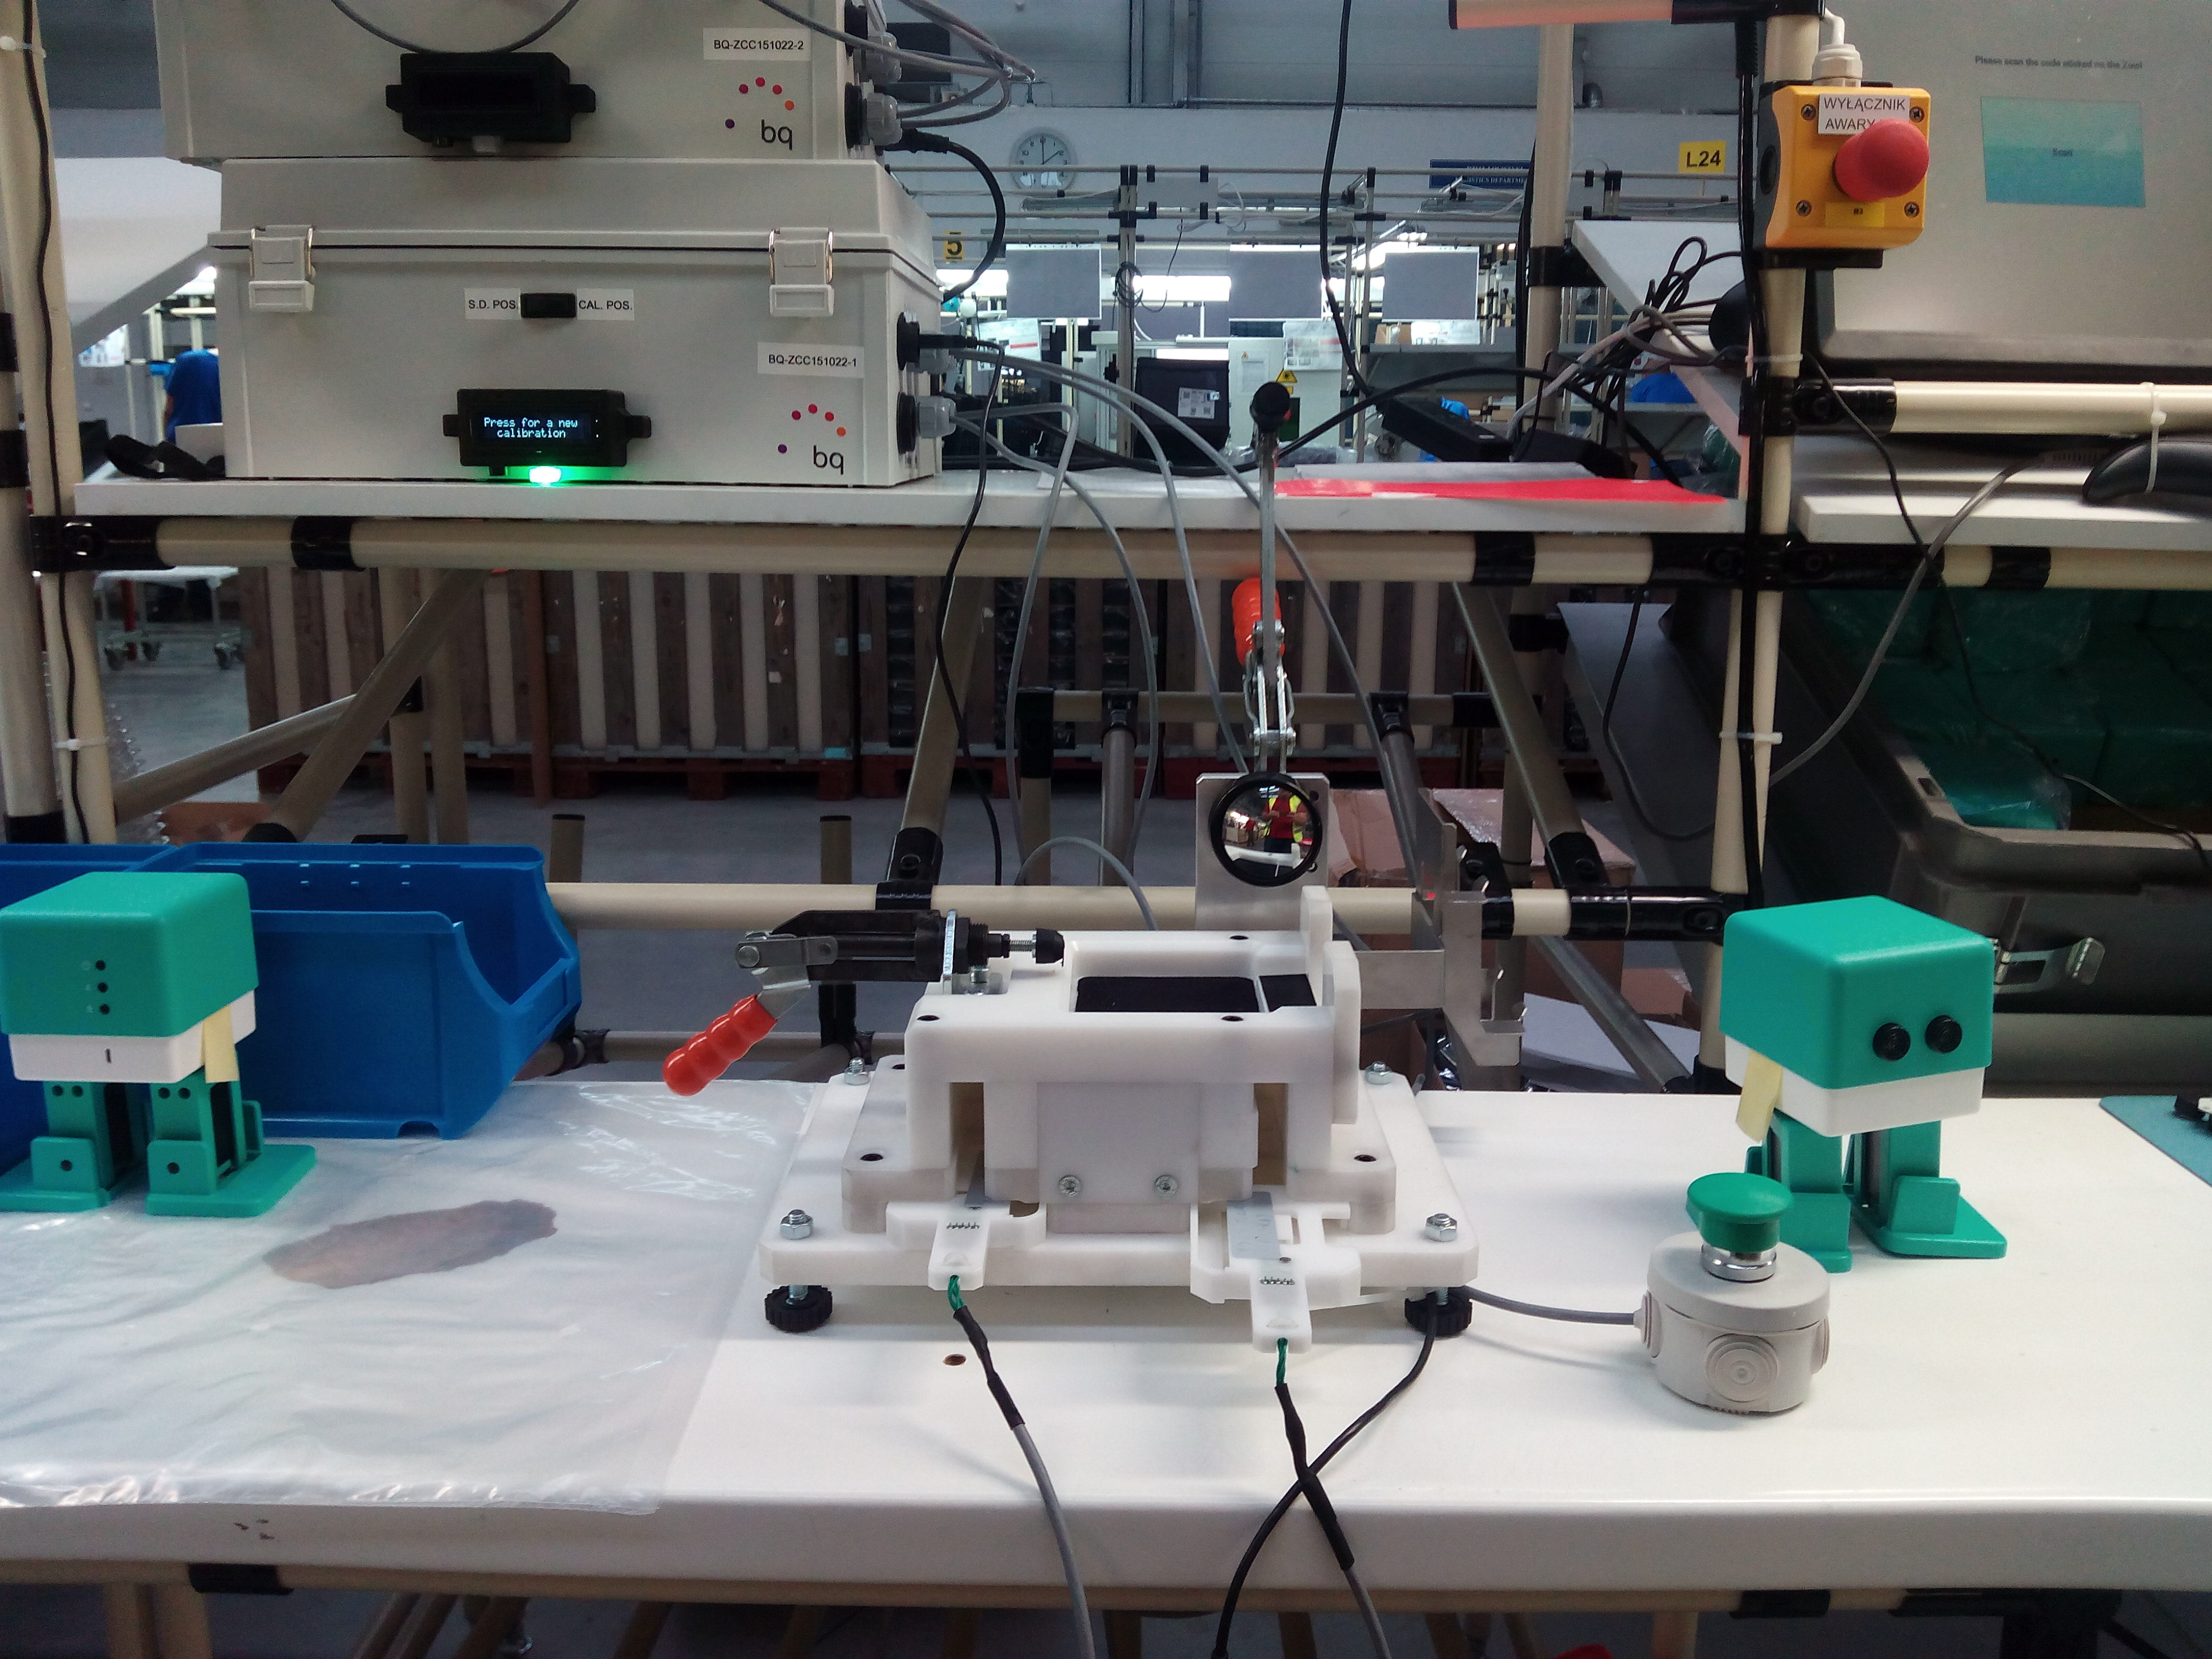
\includegraphics[width=135mm]{Figures/conc1.jpg}
\caption[Puesto de calibración en la línea de montaje]{Operadoras en línea de montaje}
\label{fig:conc1}
\end{figure}

\begin{figure}
\centering
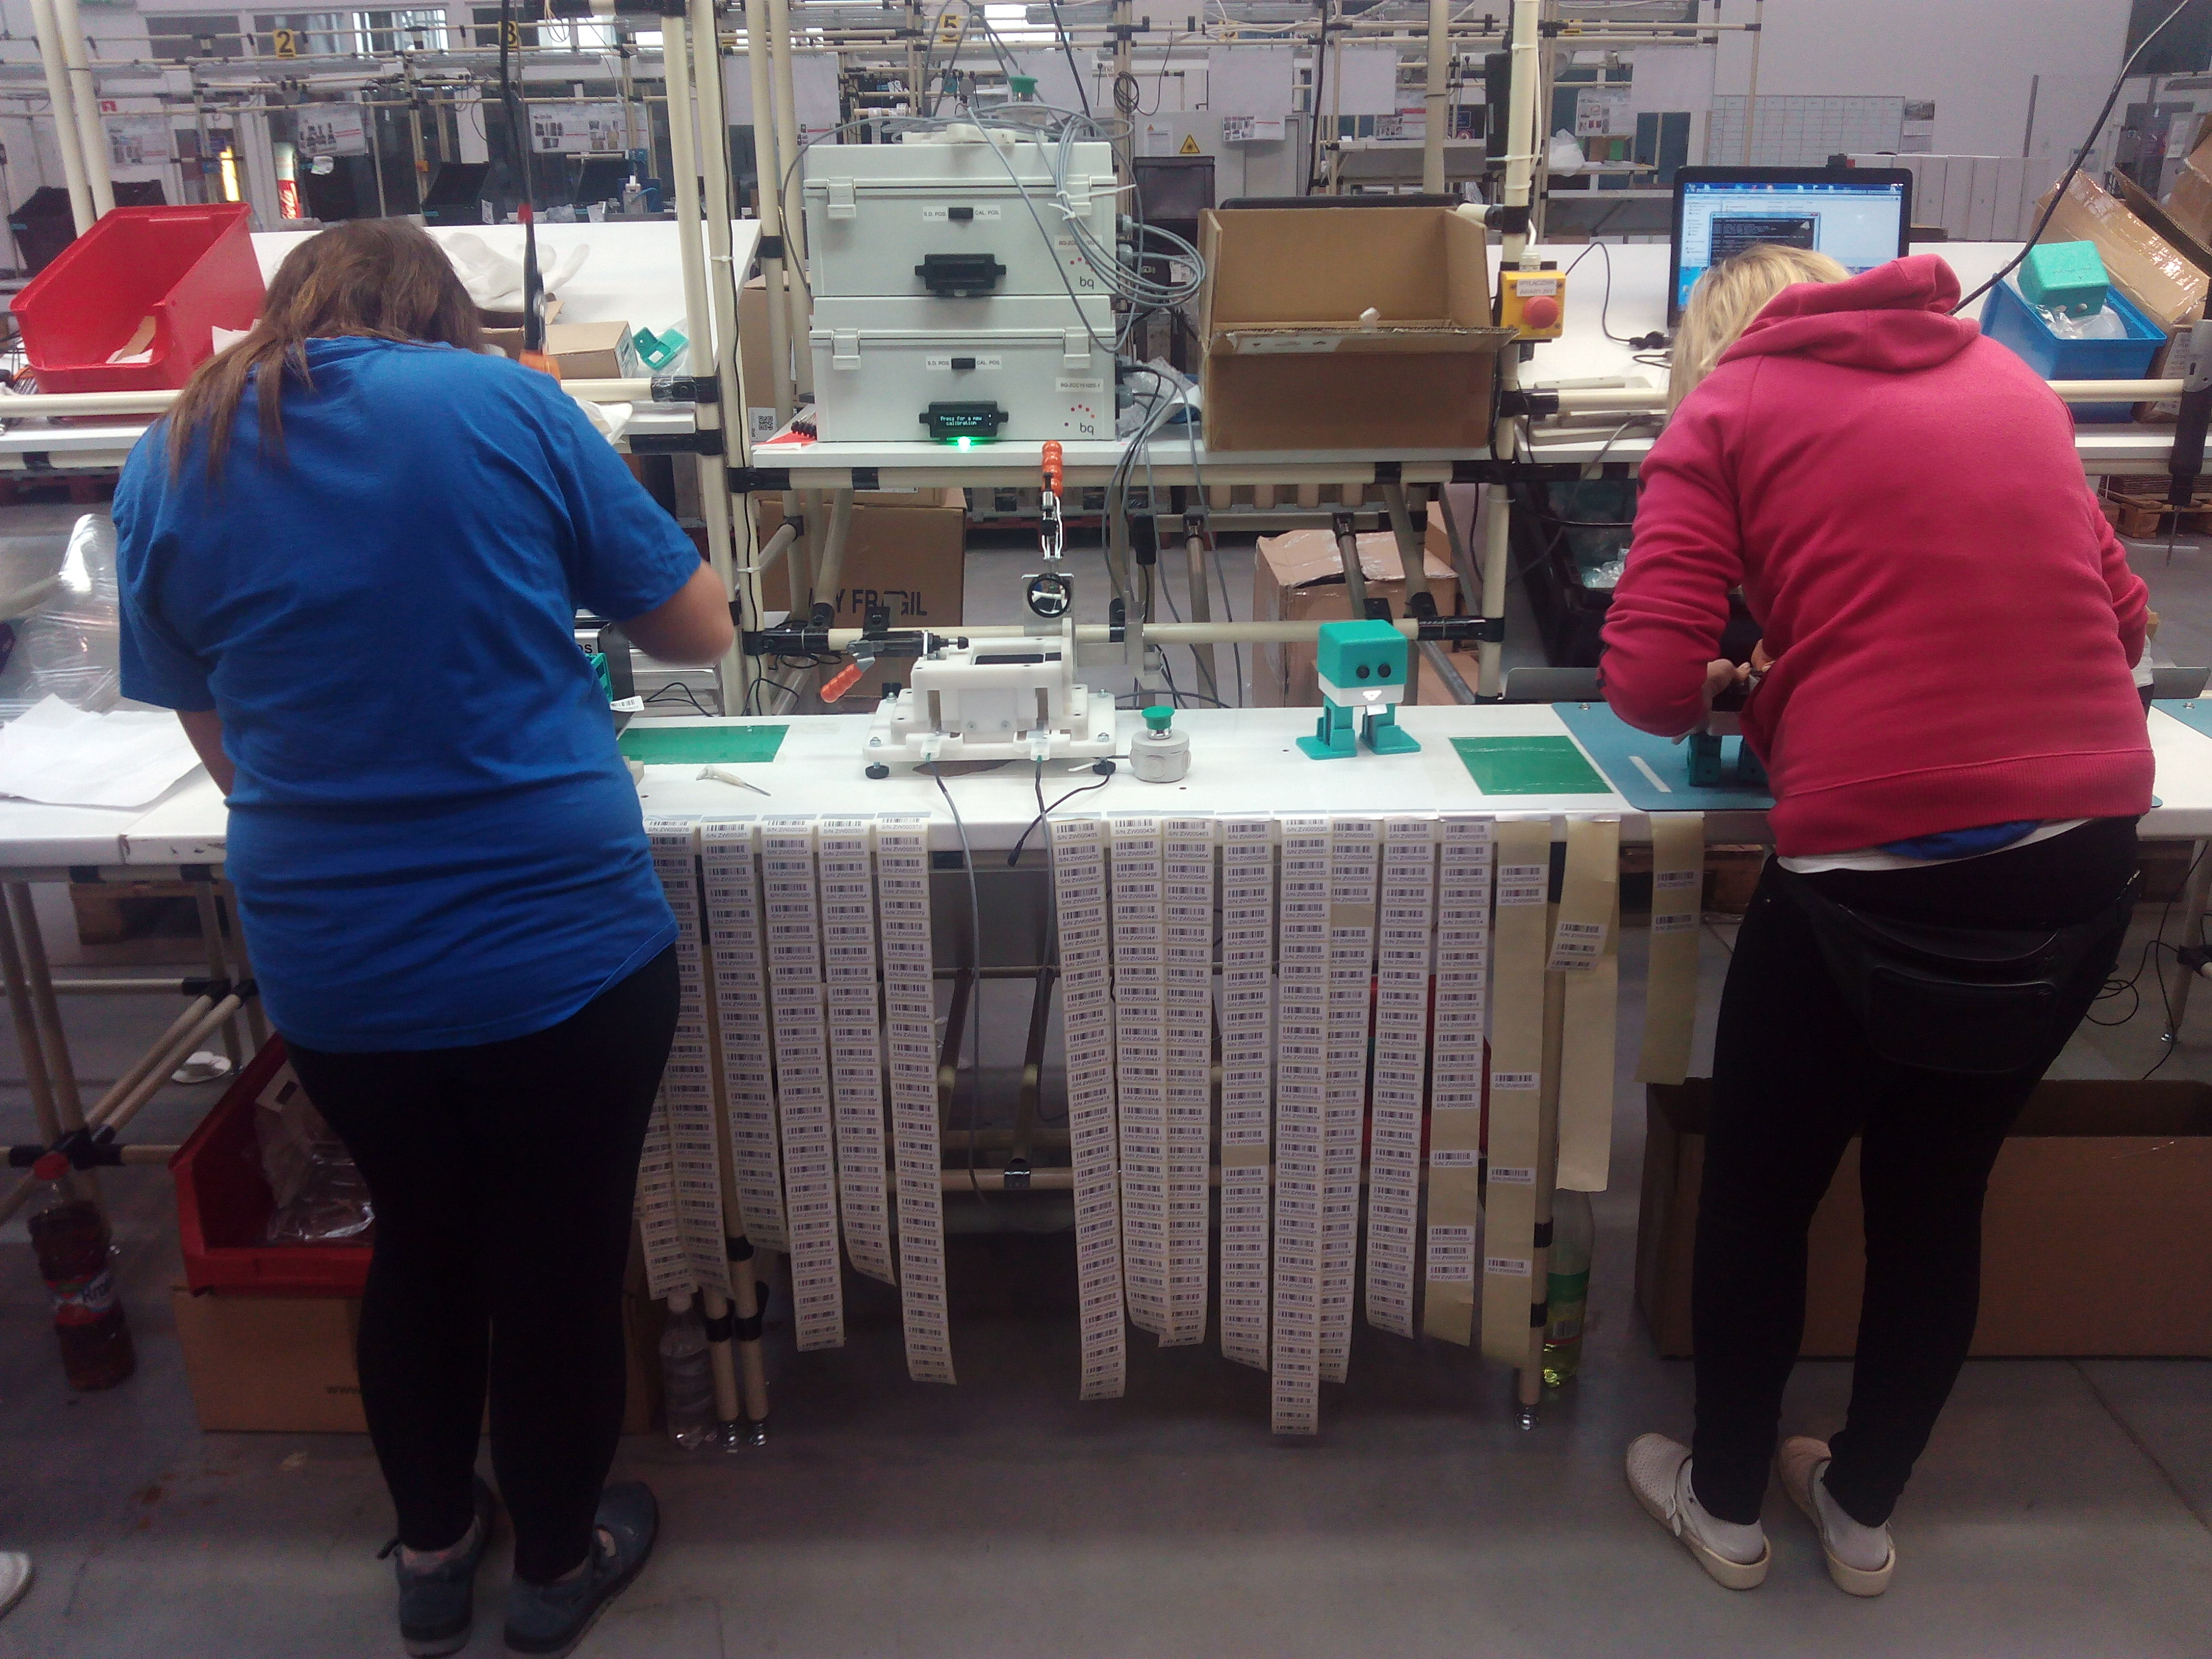
\includegraphics[width=135mm]{Figures/conc2.jpg}
\caption[Operadoras en línea de montaje]{Operadoras en línea de montaje}
\label{fig:conc2}
\end{figure}

\begin{figure}
\centering
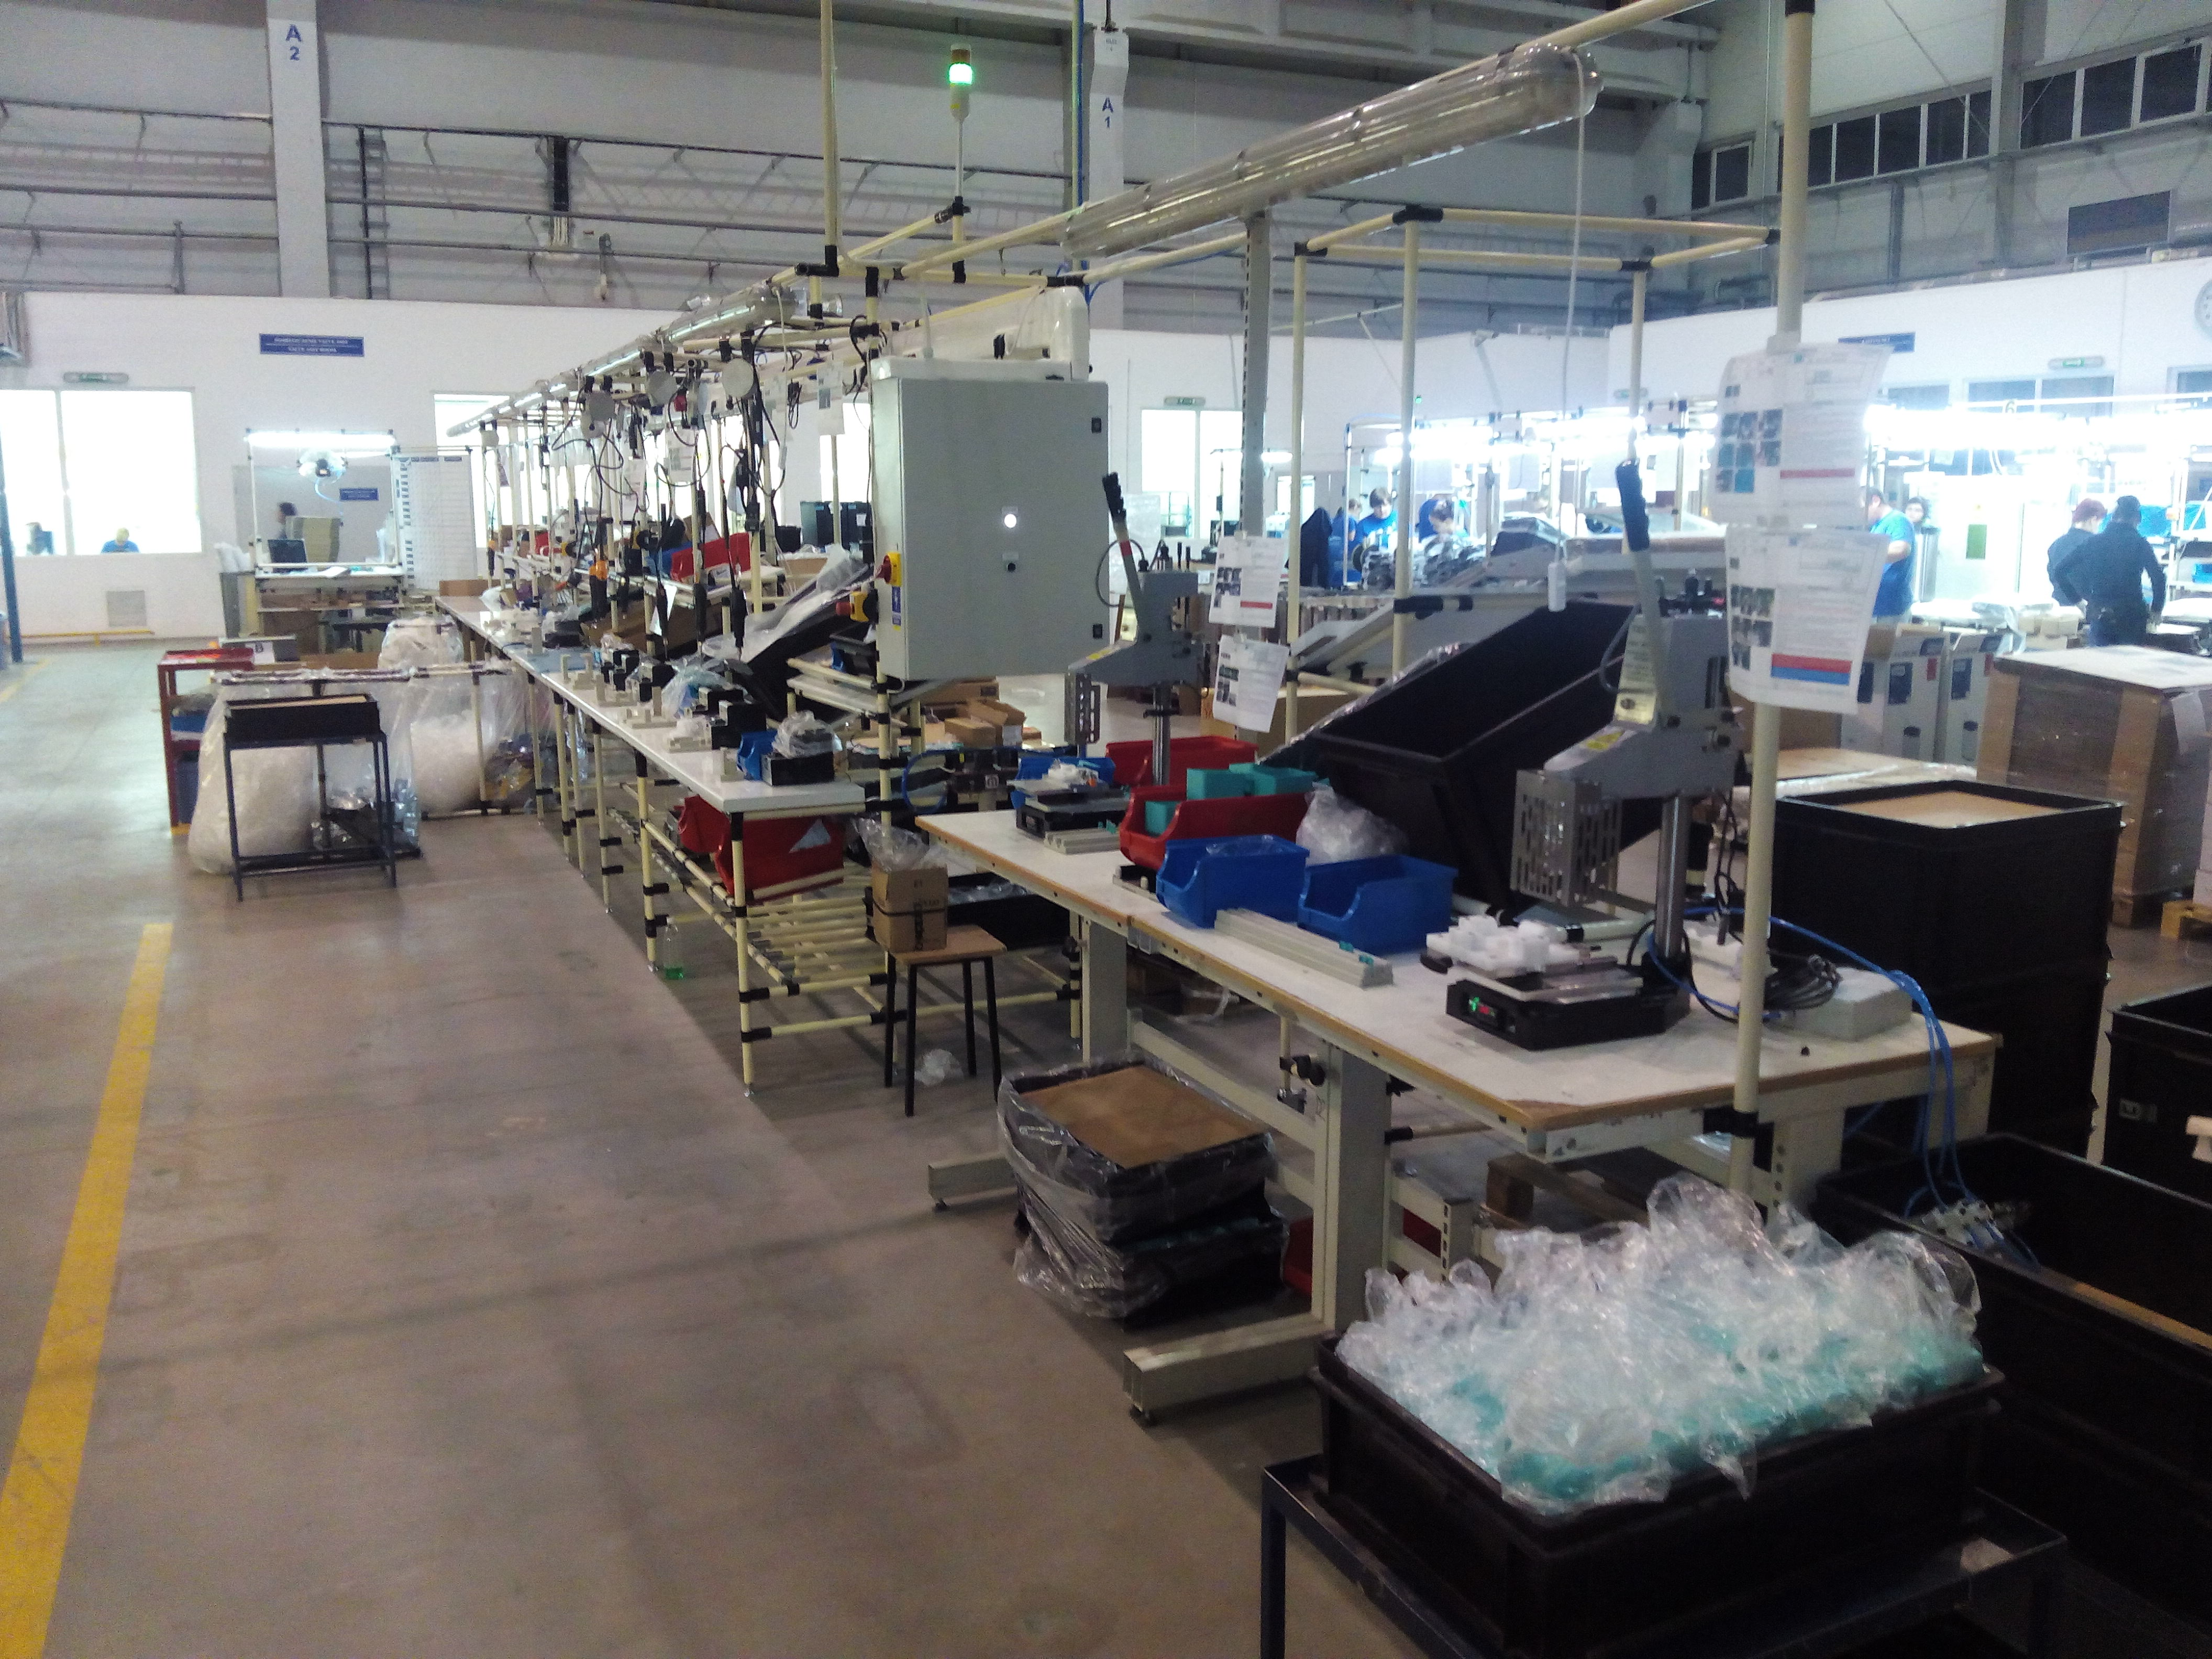
\includegraphics[width=135mm]{Figures/conc3.jpg}
\caption[Línea de montaje de Zowi en Rosti]{Línea de montaje de Zowi en Rosti}
\label{fig:conc3}
\end{figure}

El envío de dos unidades del sistema fue un acierto, en varias ocasiones fue necesario reemplazar componentes o cableado, además de las mejoras implementadas tras los primeros días de operación. Éstos contratiempos habrían sido de mayor gravedad si no se contara con el segundo armario.

Los errores más habituales fueron los producidos en el intento de programar la controladora de Zowi: Puerto USB no liberado entre Zowi y Zowi, alta del dispositivo por el SO con otro nombre de puerto, programación de Zowi sin haberlo energizado, desconexión del cable durante la programación... Los dos primeros se solucionaron de forma preventiva, mientras que para los otros dos se aplicaron medidas correctivas.

Los errores podían dejar el sistema totalmente congelado y el reinicio supone una recalibración de los zapatos, lo que consume alrededor de 2-3 minutos adicionales.

Se observa la base de datos para dos muestras de 4000 unidades -1 semana aproximadamente-. Una muestra al inicio (antes de las mejoras) y otra al final de la producción (tras mejoras). Se atiende a la forma de apagar el sistema: controlado vs. "botonzo", confiando en el buen uso de los operadores, como indicador del funcionamiento. Se muestra tambien el tiempo ciclo entre calibraciones satisfactorias. Tambien el porcentaje de "calibraciones malas". Como se ha dicho, estos elementos son indicadores, hay otros factores externos que podrían afectar a los resultados, como un mal montaje de las partes mecánicas del juguete en las etapas anteriores de la línea de montaje, o un mal uso de los operadores, entre otros. Los datos se resumen en la Tabla \ref{tableResults}.

\begin{table}[h]
\centering
\begin{tabular}{l c c}
\toprule
 & \textbf{Pre-mejoras} & \textbf{Post-mejoras} \\
\midrule
Tiempo calibración medio & 81s & 50s \\
Calibraciones a la primera & 98.61\% & 99.13\% \\
Calibraciones OK & 99.76\% & 99.89\% \\
Apagados "forzados" & 63\% & 43\% \\
Sistema recuperado error & - & 35\% \\
\bottomrule\\
\end{tabular}
\caption{Conclusiones y resultados}
\label{tableResults}
\end{table}

\section{Trabajos futuros}

Tras la finalización de la producción inicial, se trae la fabricación del robot Zowi a España, los armarios de calibración y los bancos finales fueron enviados a la fábrica que BQ tiene en Noáin (Navarra), dónde continúan funcionando.

El último prototipo creado fue actualizado con todos los cambios desarrollados para la versión final y se emplea en el SAT de BQ, en Rivas-Vaciamadrid, utilizando el utillaje diseñado en la fase de desarrollo, Anexo \ref{app:piezas}.

Hablar de futuras mejoras sobre éste mismo sistema no tiene sentido ya que el proyecto quedó cerrado y hay otras etapas más lentas en la línea de montaje. Sin embargo, si que se podría haber logrado un mejor diseño, como se comenta a continuación.

Una posible y elegante mejora en la velocidad sería el empleo de un PID en la lectura-actuación de las posición de los servos en lugar del método por iteraciones empleado.

De cara a otros proyectos utilizando arquitecturas similares (Raspberry y Arduino), donde los plazos y tiempos no jueguen un papel tan importante entre los requisitos, habría algunos puntos a tener en cuenta tras lo aprendido en la realización de éste proyecto:

\begin{itemize}
  \item Trabajar en el software: Implementar un logger en las mismas scripts de python y un mayor uso de try-except y comprobaciones que permitan conocer con mayor detalle la traza de operación.
  \item En la misma línea que el punto anterior, utilizar un campo en la estructura de la base de datos para representar qué se está guardando en dicha entrada, ésto permitiría identificar facilmente los diferentes errores, warnings, mensajes informativos...
  \item Desarrollar un pequeño protocolo o herramienta para la comunicación entre Python y Arduino por serie, con una gestión de errores para validación en la interpretación. Dicho protocolo haría más fácil definir en ambos dispositivos las instrucciones que se desean implementar para la comunicación.
  \item El empleo de un reloj RTC (Real time clock) en la Raspberry evitaría la desconfiguración de la hora cuando ésta no tiene acceso a internet y no se puede utilizar NTP para mantener su hora sincronizada.
\end{itemize}


%----------------------------------------------------------------------------------------
%	THESIS CONTENT - APPENDICES
%----------------------------------------------------------------------------------------

\appendix % Cue to tell LaTeX that the following "chapters" are Appendices

% Include the appendices of the thesis as separate files from the Appendices folder
% Uncomment the lines as you write the Appendices


\chapter{Manual de usuario} % Main appendix title

\label{app:usermanual} % For referencing this appendix elsewhere, use \ref{AppendixA}

Manual de usuario entregado a la empresa contratada para la fabricación, destinado a los operadores de la fábrica.

\newpage

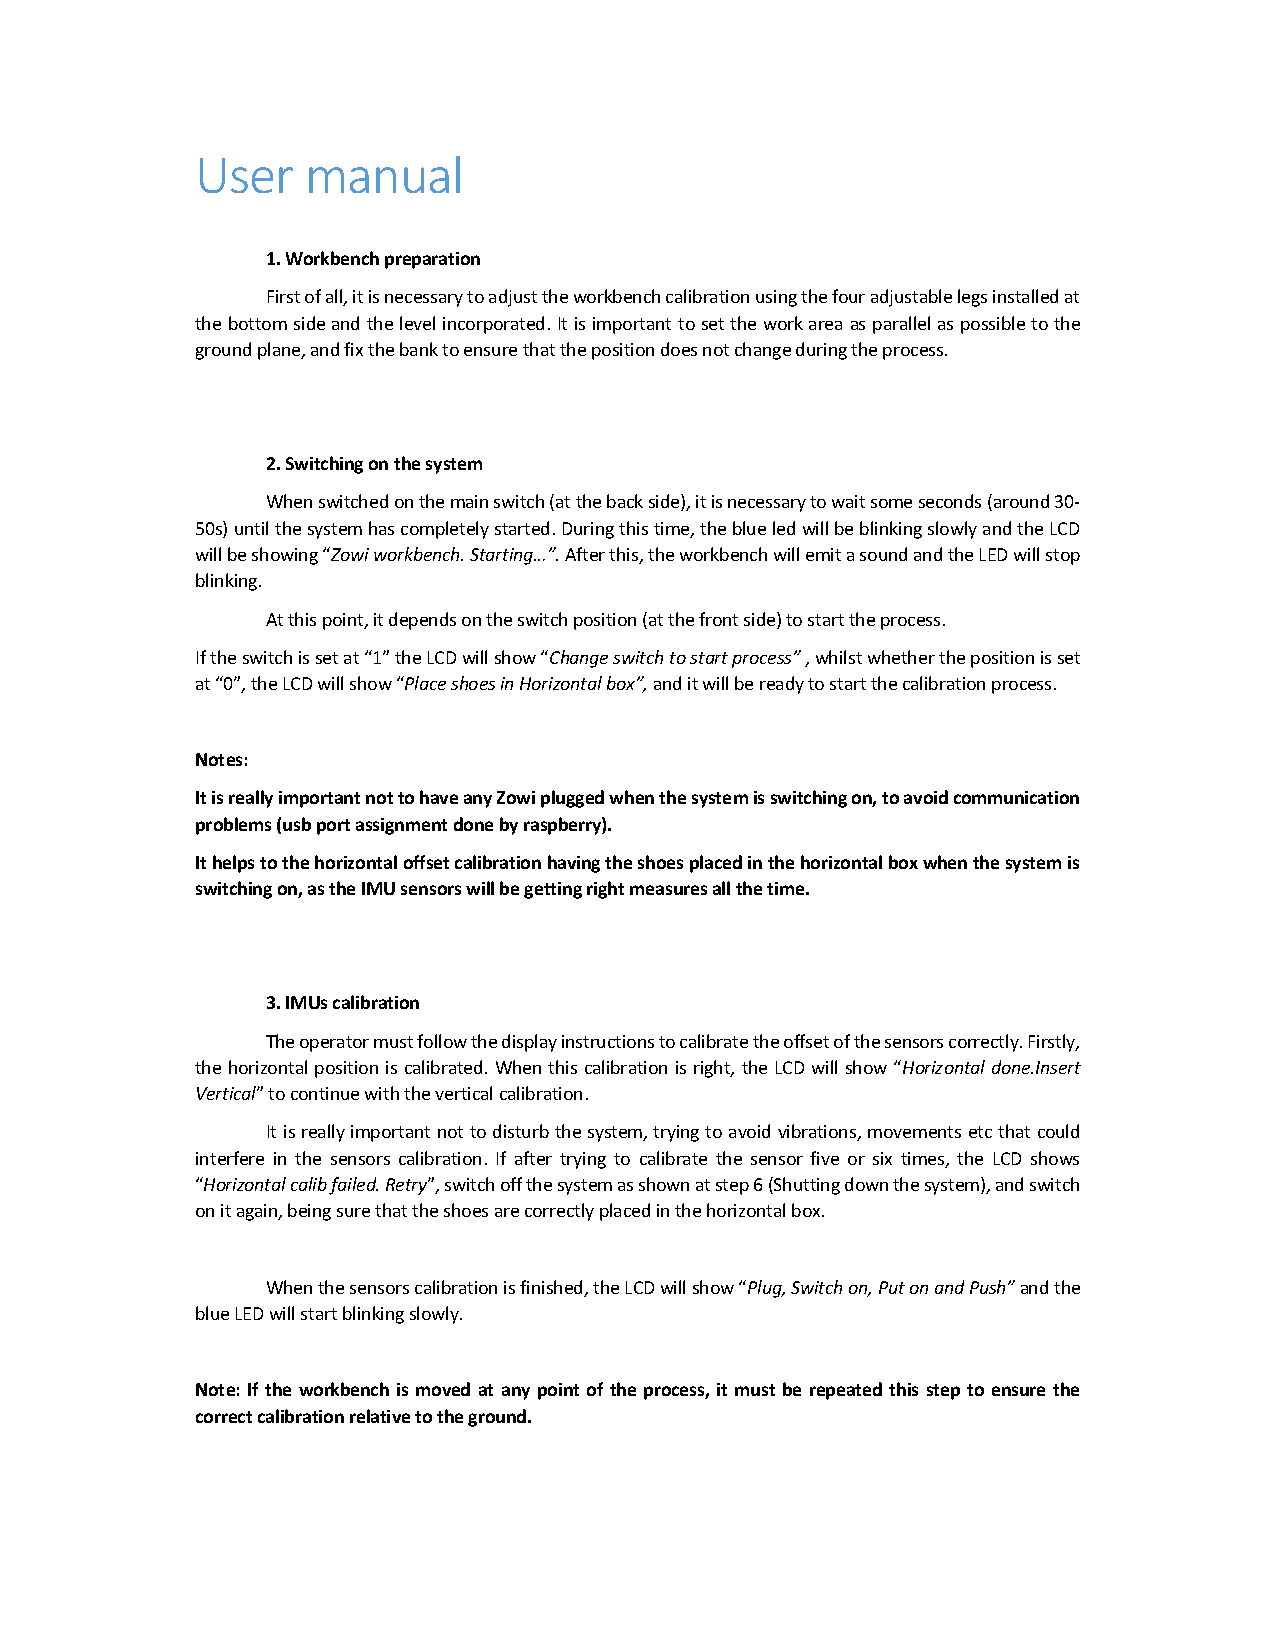
\includepdf[pages=-, pagecommand={}]{Appendices/externos/User-manual.pdf}


\chapter{Planos Eléctricos: Armario 1} % Main appendix title

\label{app:planosElectricos} % For referencing this appendix elsewhere, use \ref{AppendixA}

Planos eléctricos del armario 1.

\newpage

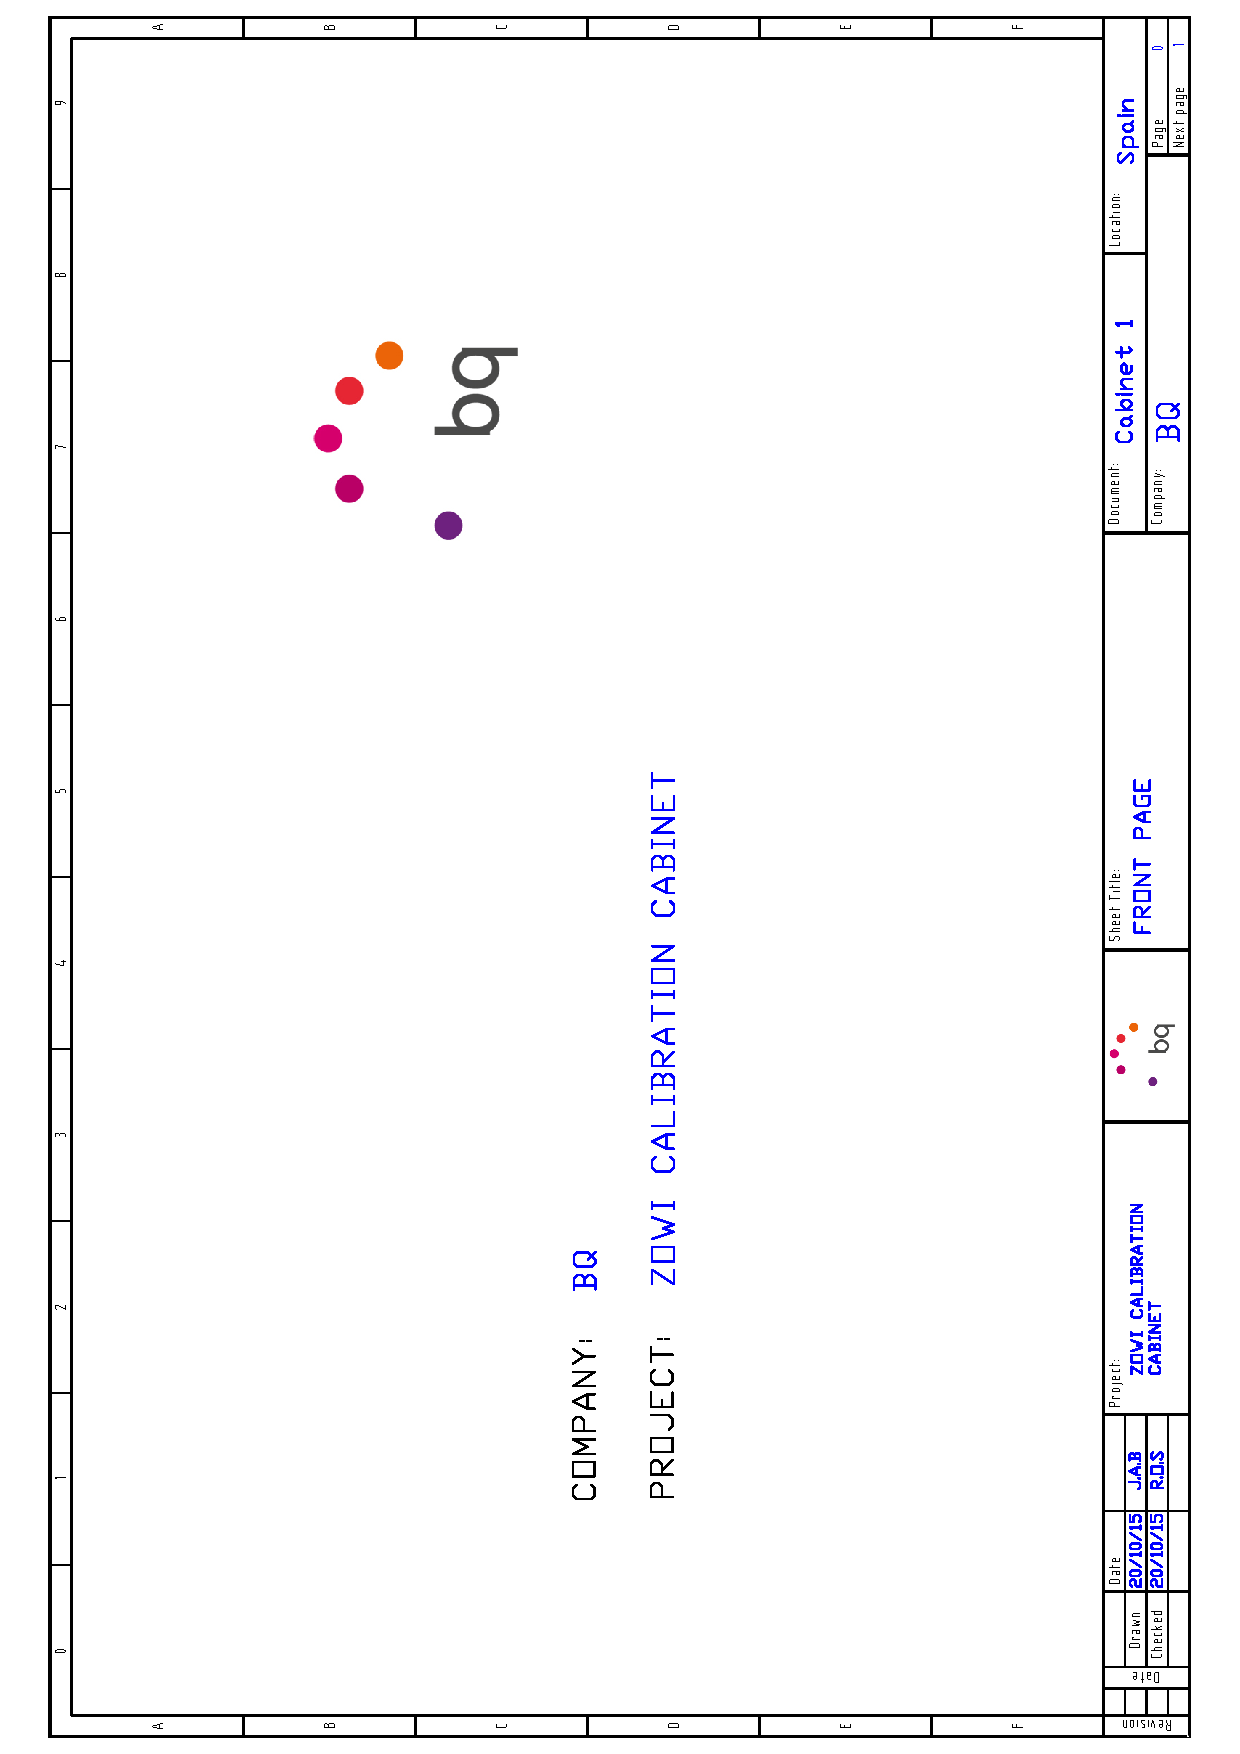
\includepdf[pages=-]{Appendices/externos/PlanosElectricos/cab1.pdf}


\chapter{Planos Eléctricos: Armario 2} % Main appendix title

\label{app:planosEle2} % For referencing this appendix elsewhere, use \ref{AppendixA}

Planos eléctricos del armario 2.

\newpage

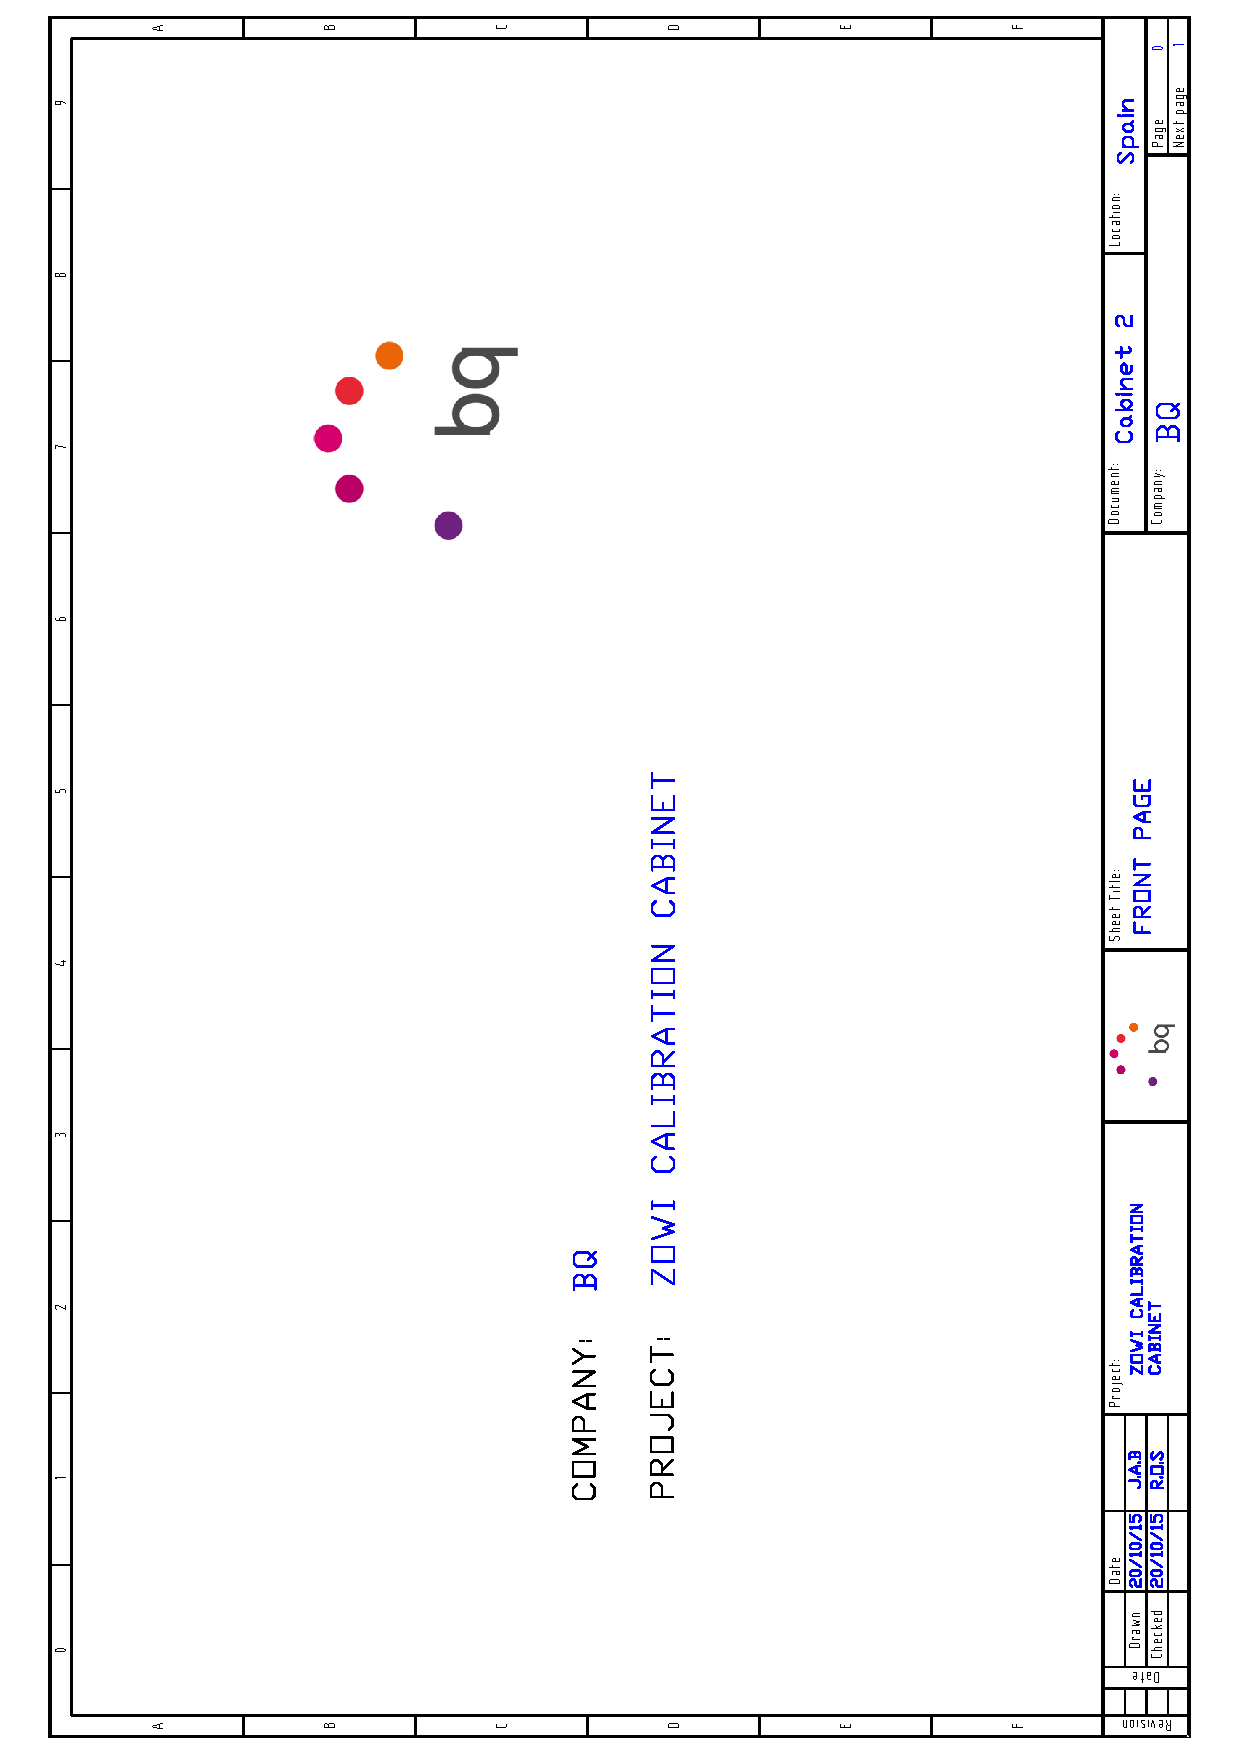
\includepdf[pages=-]{Appendices/externos/PlanosElectricos/cab2.pdf}


\chapter{Mega PINOUT} % Main appendix title

\label{app:pinoutMega} % For referencing this appendix elsewhere, use \ref{AppendixA}

Pinout de Freaduino Mega2560.

\newpage

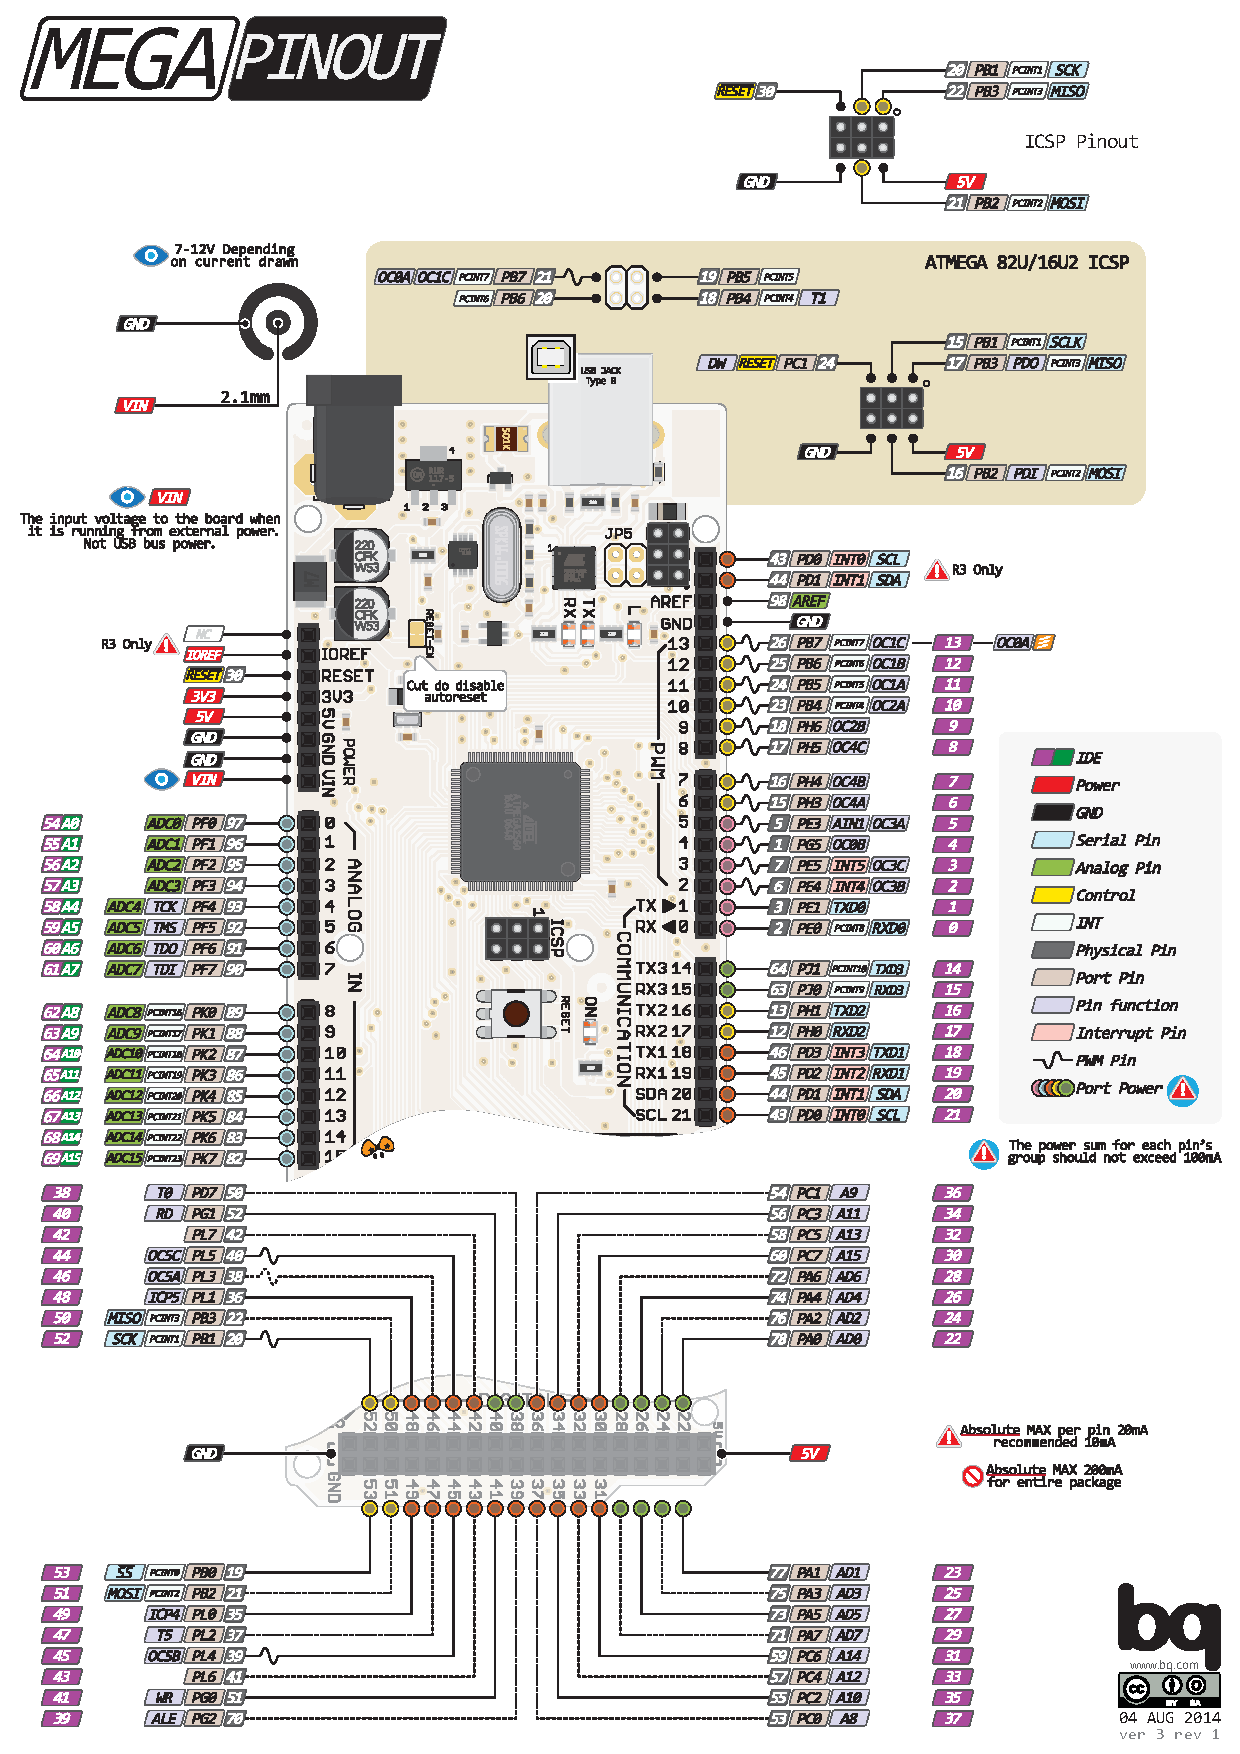
\includepdf[pages=-]{Appendices/externos/megapdf.pdf}


\chapter{Mega Custom Shield} % Main appendix title

\label{app:pcbFiles} % For referencing this appendix elsewhere, use \ref{AppendixA}

Esquemático y gerbers del shield diseñedo para Mega.

\newpage

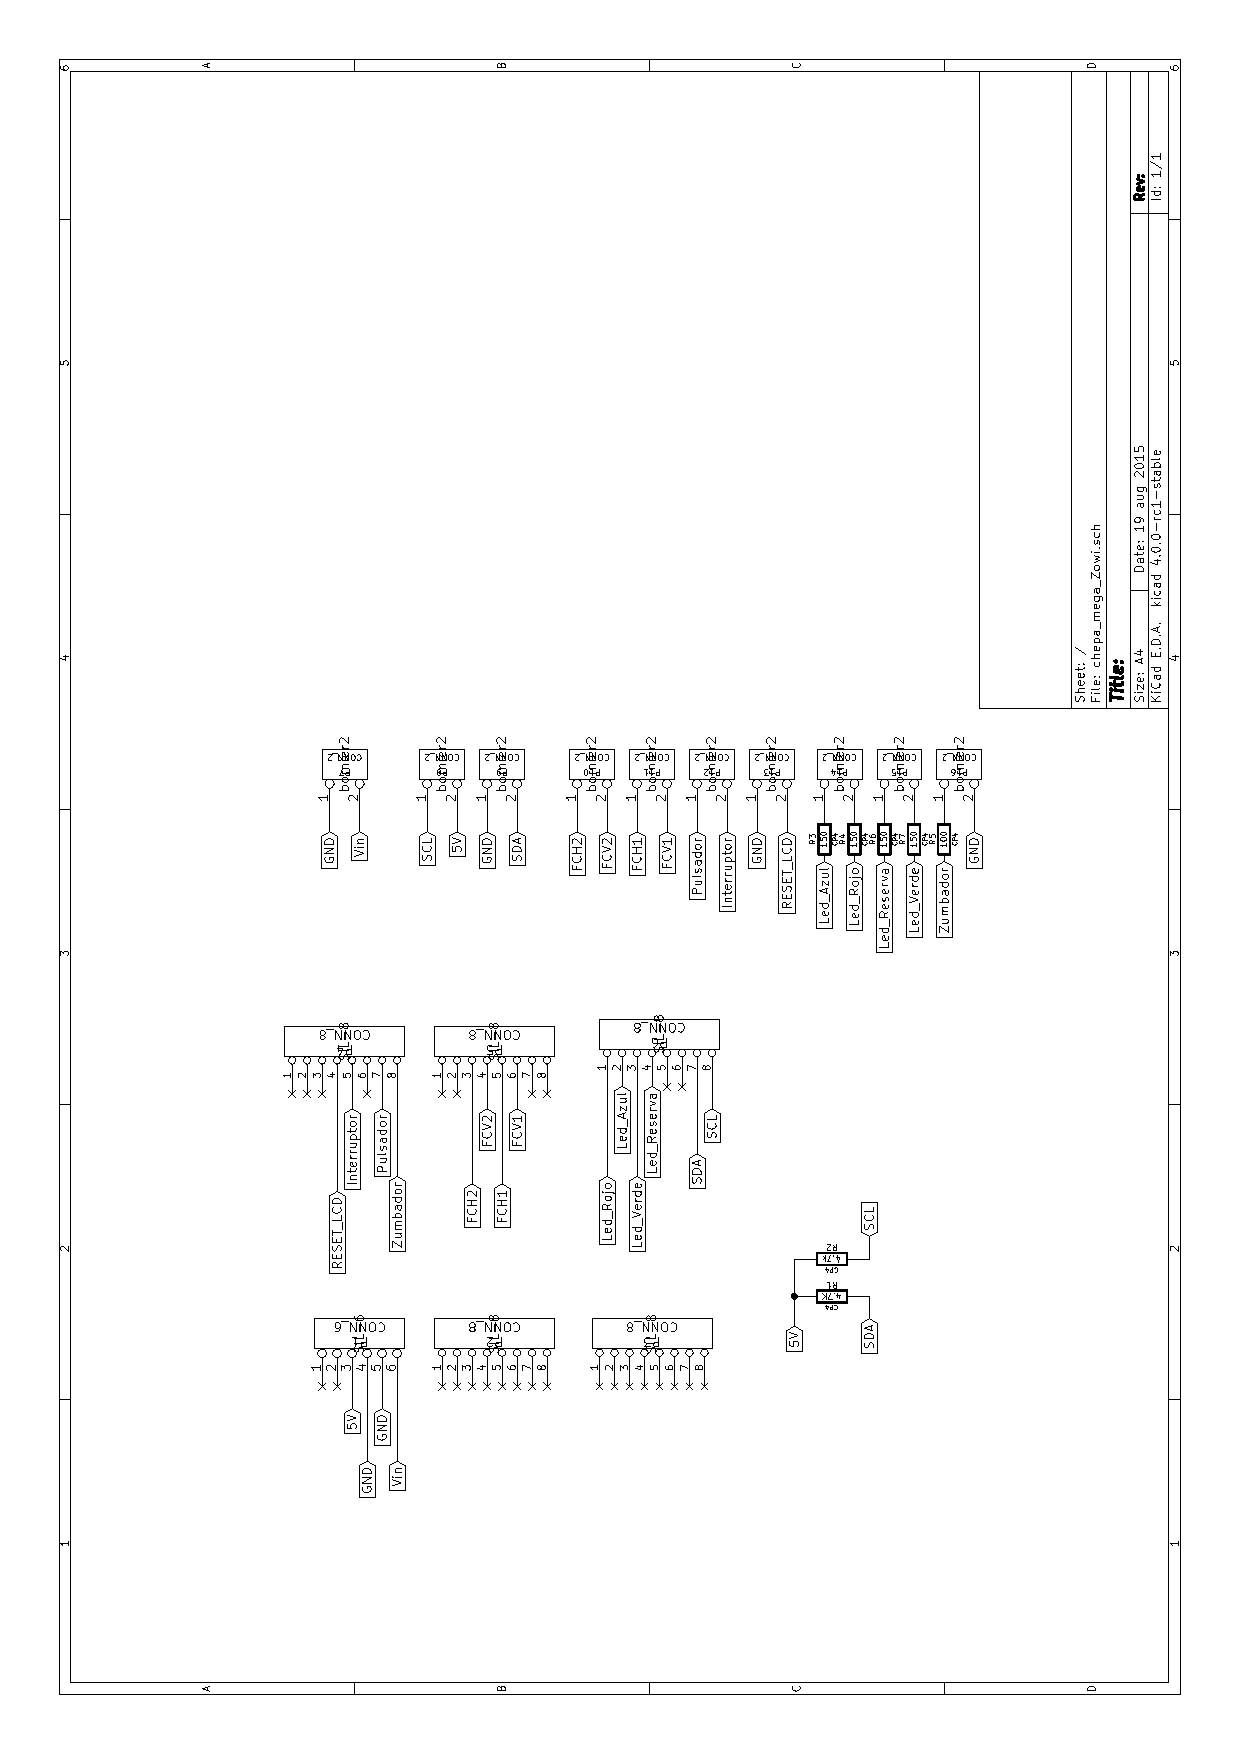
\includepdf[pages=-]{Appendices/externos/PCB/Schematic.pdf}
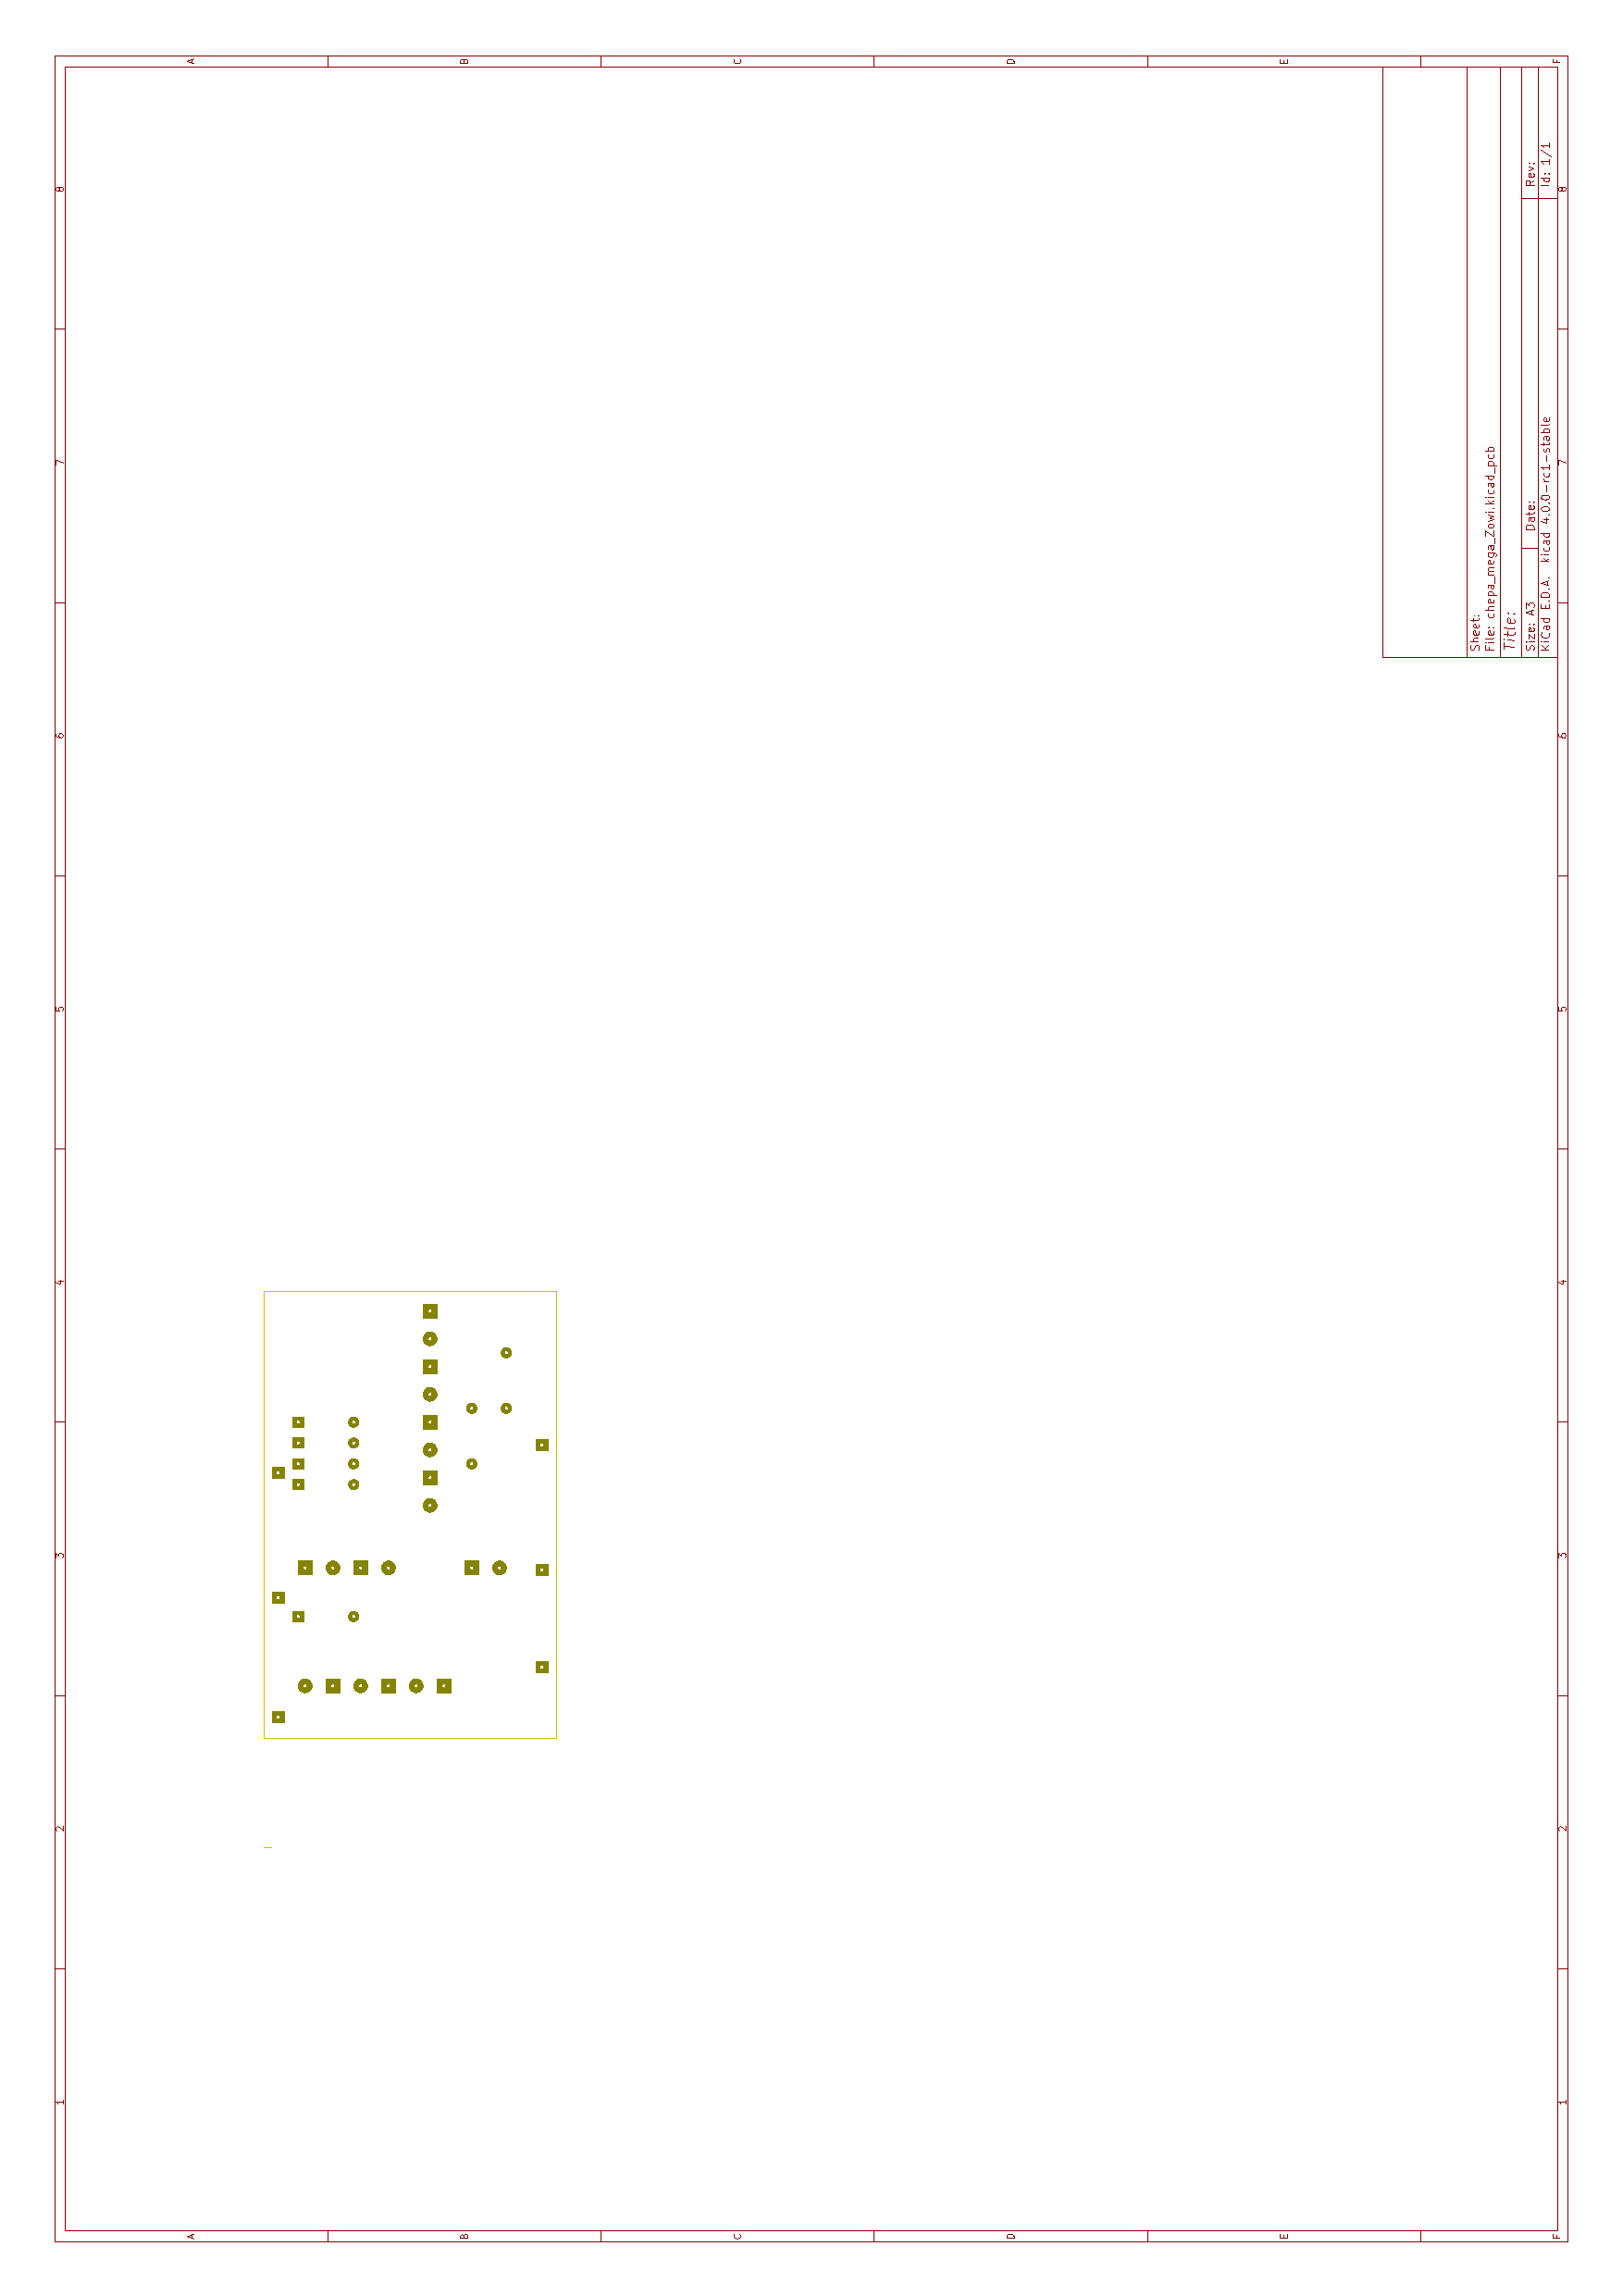
\includepdf[pages=-]{Appendices/externos/PCB/Gerbers.pdf}


\chapter{Máquina de estados Mega} % Main appendix title

\label{app:megadiag} % For referencing this appendix elsewhere, use \ref{AppendixA}

Diagrama de la máquina de estados implementada en Mega.

\newpage

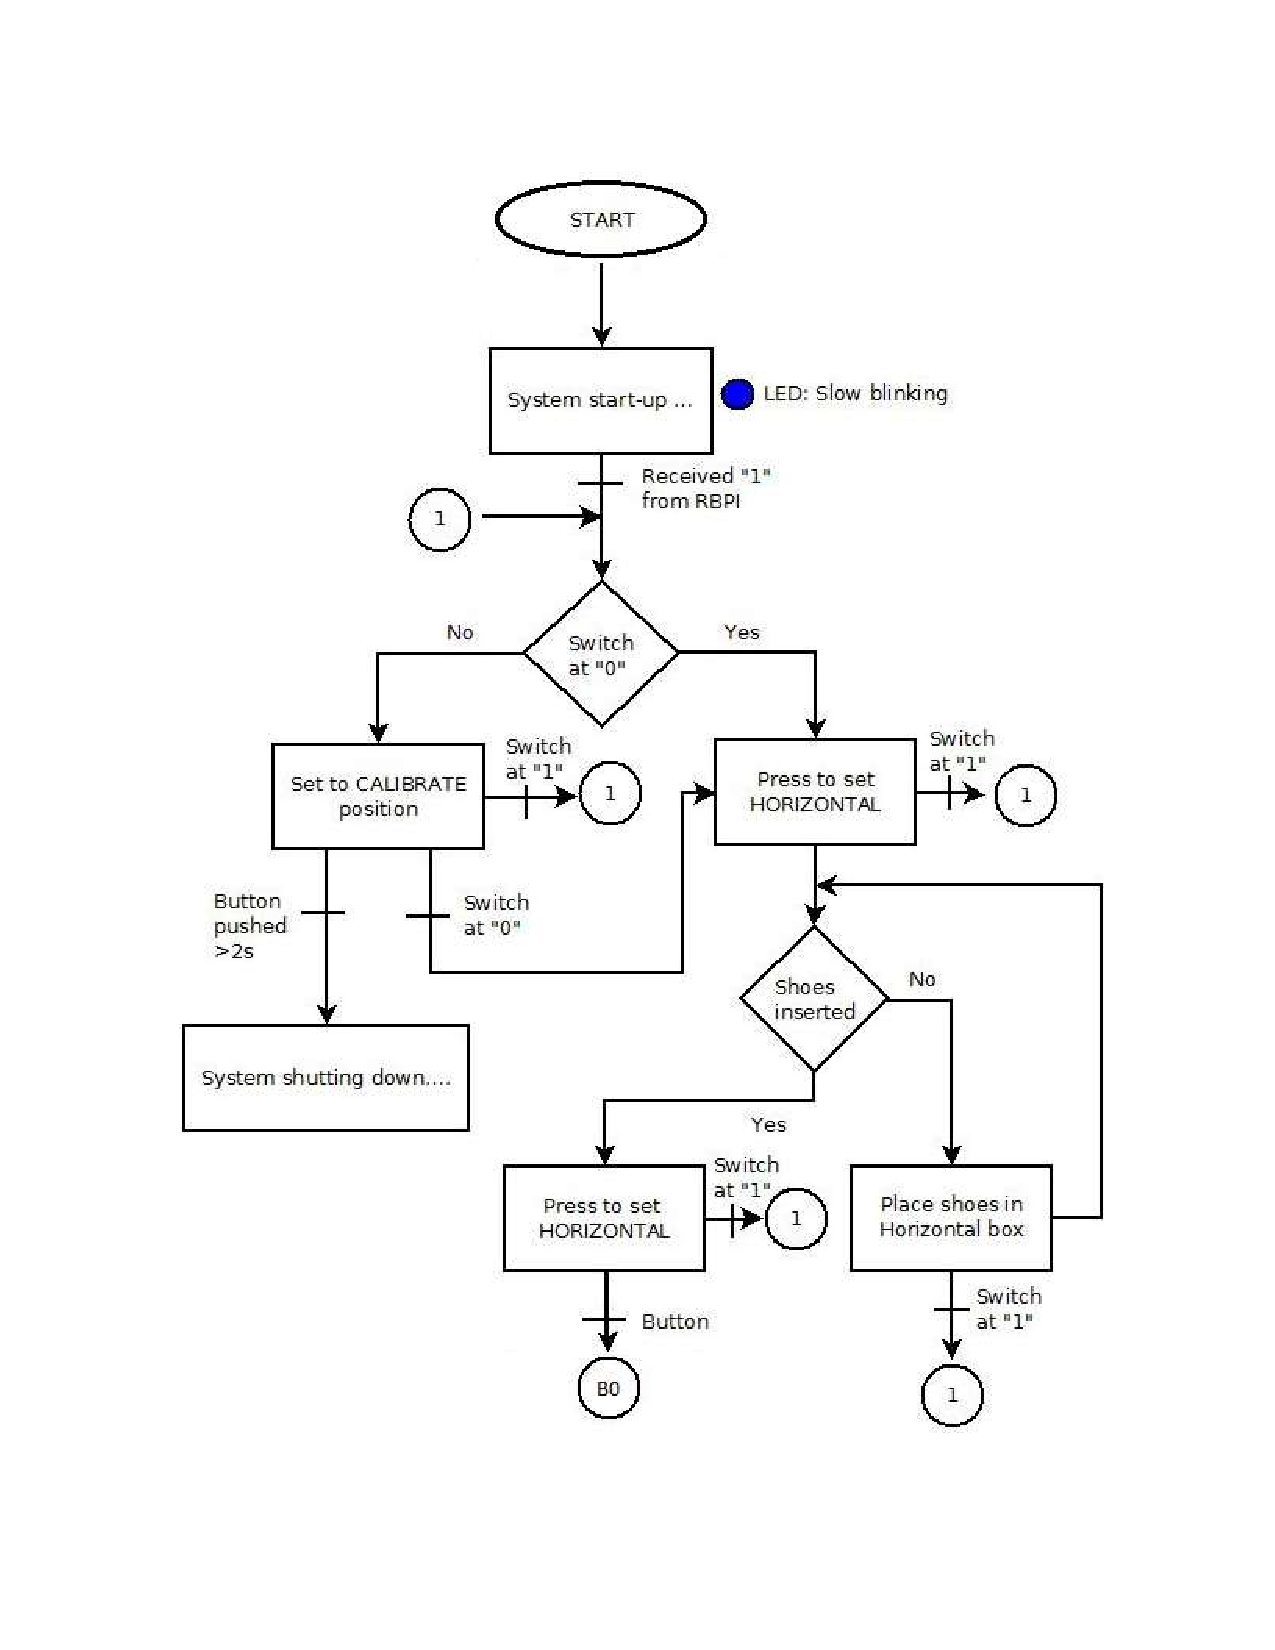
\includepdf[pages=-, pagecommand={}]{Appendices/externos/DiagramaMEGA/MegaDiag.pdf}


\chapter{Configuración IMUS} % Main appendix title

\label{app:imuvalues} % For referencing this appendix elsewhere, use \ref{AppendixA}

Valores máximos y mínimos de la calibración de las IMUs instaladas en los dos armarios. Además de información de sus pines SA0, selector de direcciones de esclavo I\textsuperscript{2}C.

\newpage

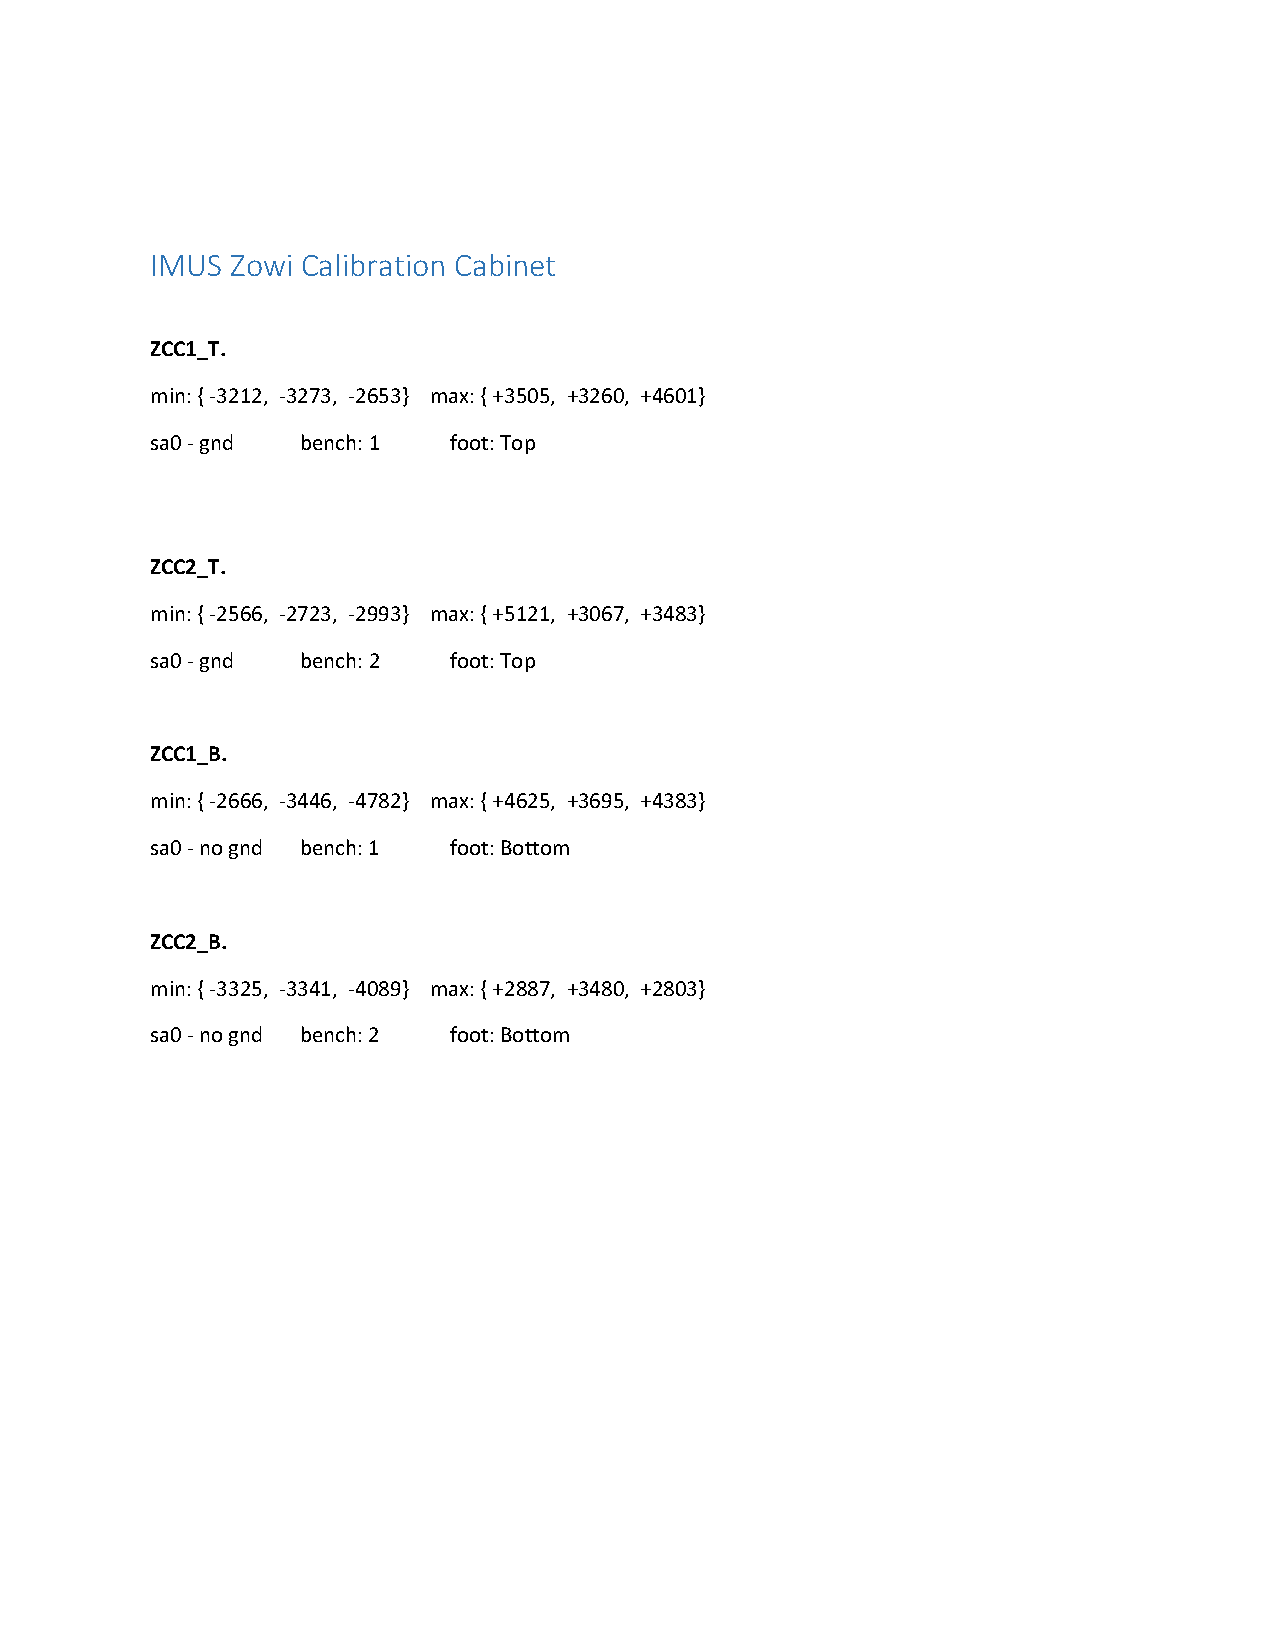
\includepdf[pages=-, pagecommand={}]{Appendices/externos/IMU-values.pdf}


\chapter{Estructura base de datos} % Main appendix title

\label{app:dbsctruct} % For referencing this appendix elsewhere, use \ref{AppendixA}

En este documento se muestra la estructura de la base de datos, además de las direcciones de la EEPROM de Zowi donde se guardan las posiciones ``offset'' de los servos.

\newpage

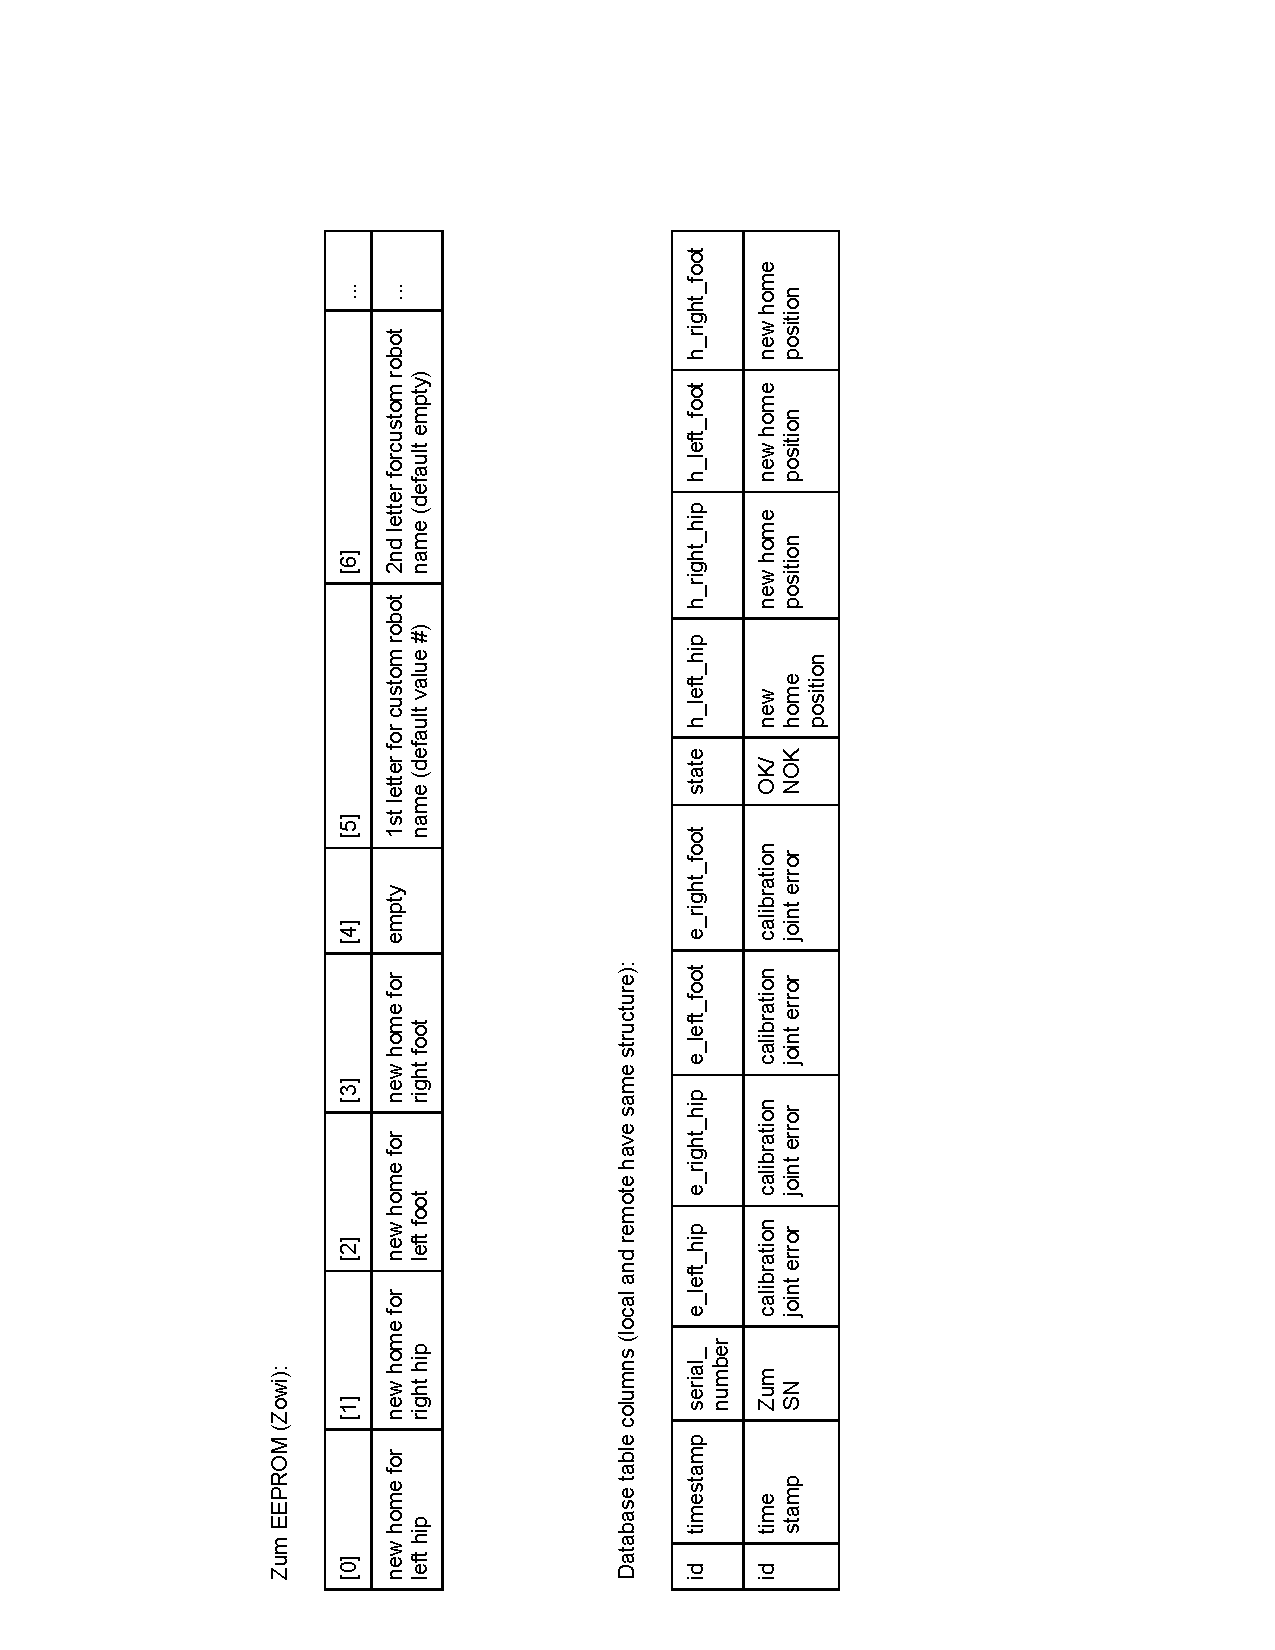
\includepdf[pages=-, pagecommand={}]{Appendices/externos/db-struct.pdf}


\chapter{BOM de los armarios finales} % Main appendix title

\label{app:BOM} % For referencing this appendix elsewhere, use \ref{AppendixA}

Desglose de precios de los componentes del sistema final, para ambos armarios.

\newpage

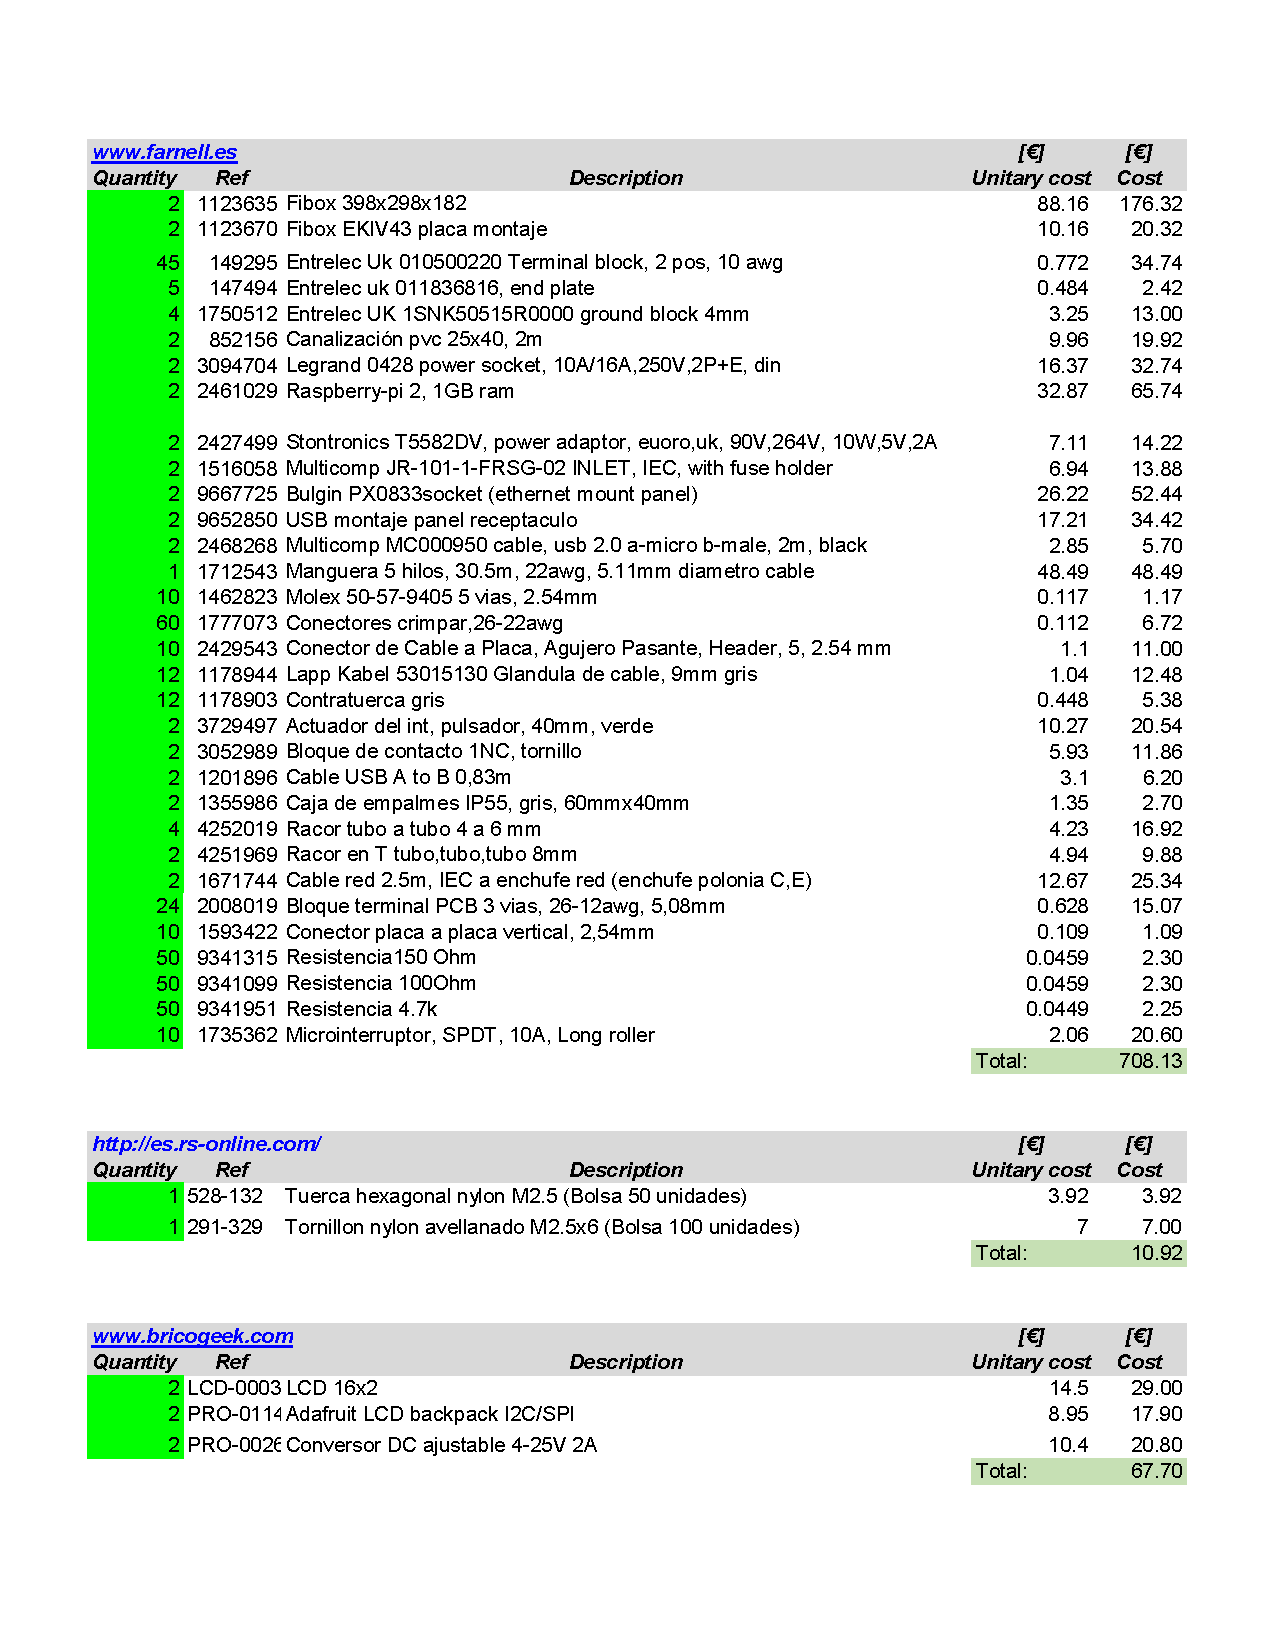
\includepdf[pages=-, pagecommand={}]{Appendices/externos/bomfinal.pdf}


\chapter{Piezas Impresas} % Main appendix title

\label{app:piezas} % For referencing this appendix elsewhere, use \ref{AppendixA}

Piezas diseñadas e impresas para el desarrollo. El prototipo del sistema previo a la versión final (funcionando en el SAT de Rivas) utiliza estas piezas.

\newpage

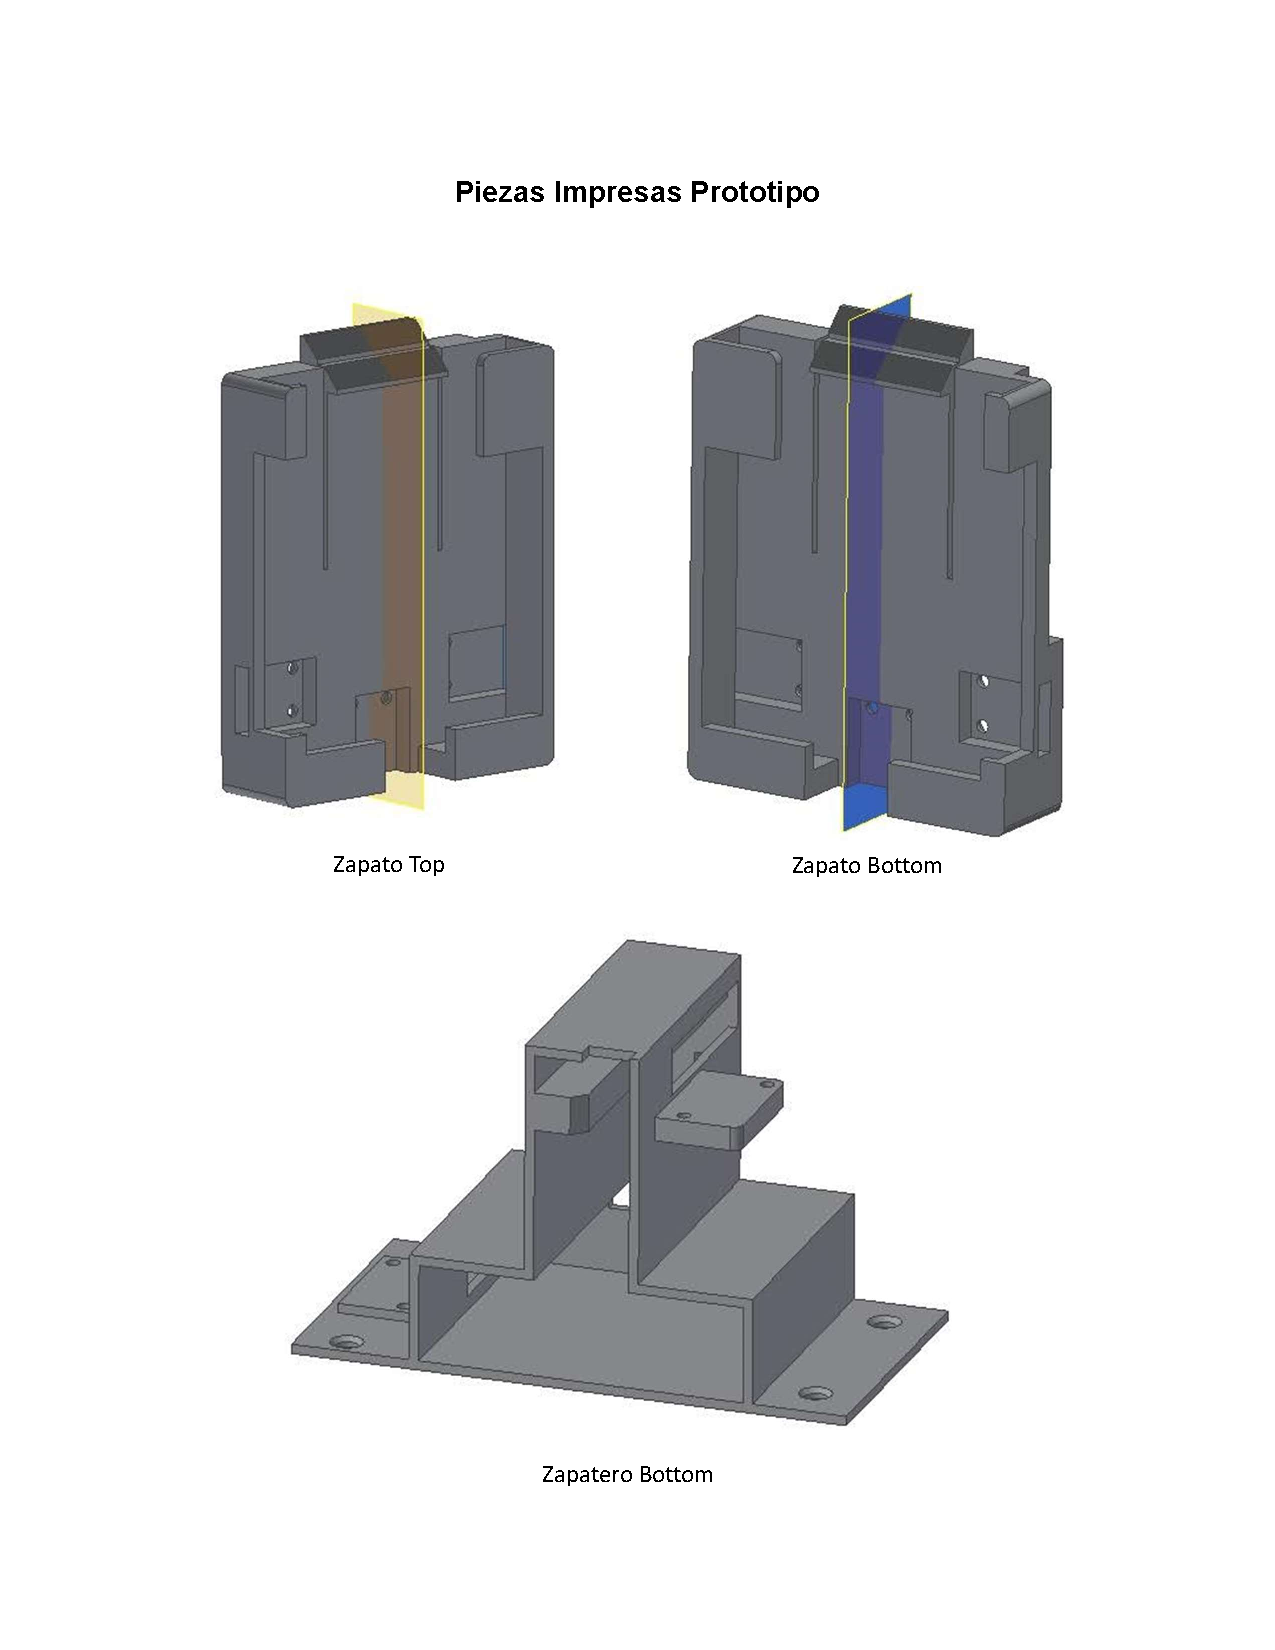
\includepdf[pages=-, pagecommand={}]{Appendices/externos/piezas.pdf}


\chapter{Fichero running.sh} % Main appendix title

\label{app:running} % For referencing this appendix elsewhere, use \ref{AppendixA}

Fichero running.sh, encargado de lanzar la script principal de python y relanzarla si esta es interrumpida. Debe estar en /etc/init.d/running.sh.

\newpage

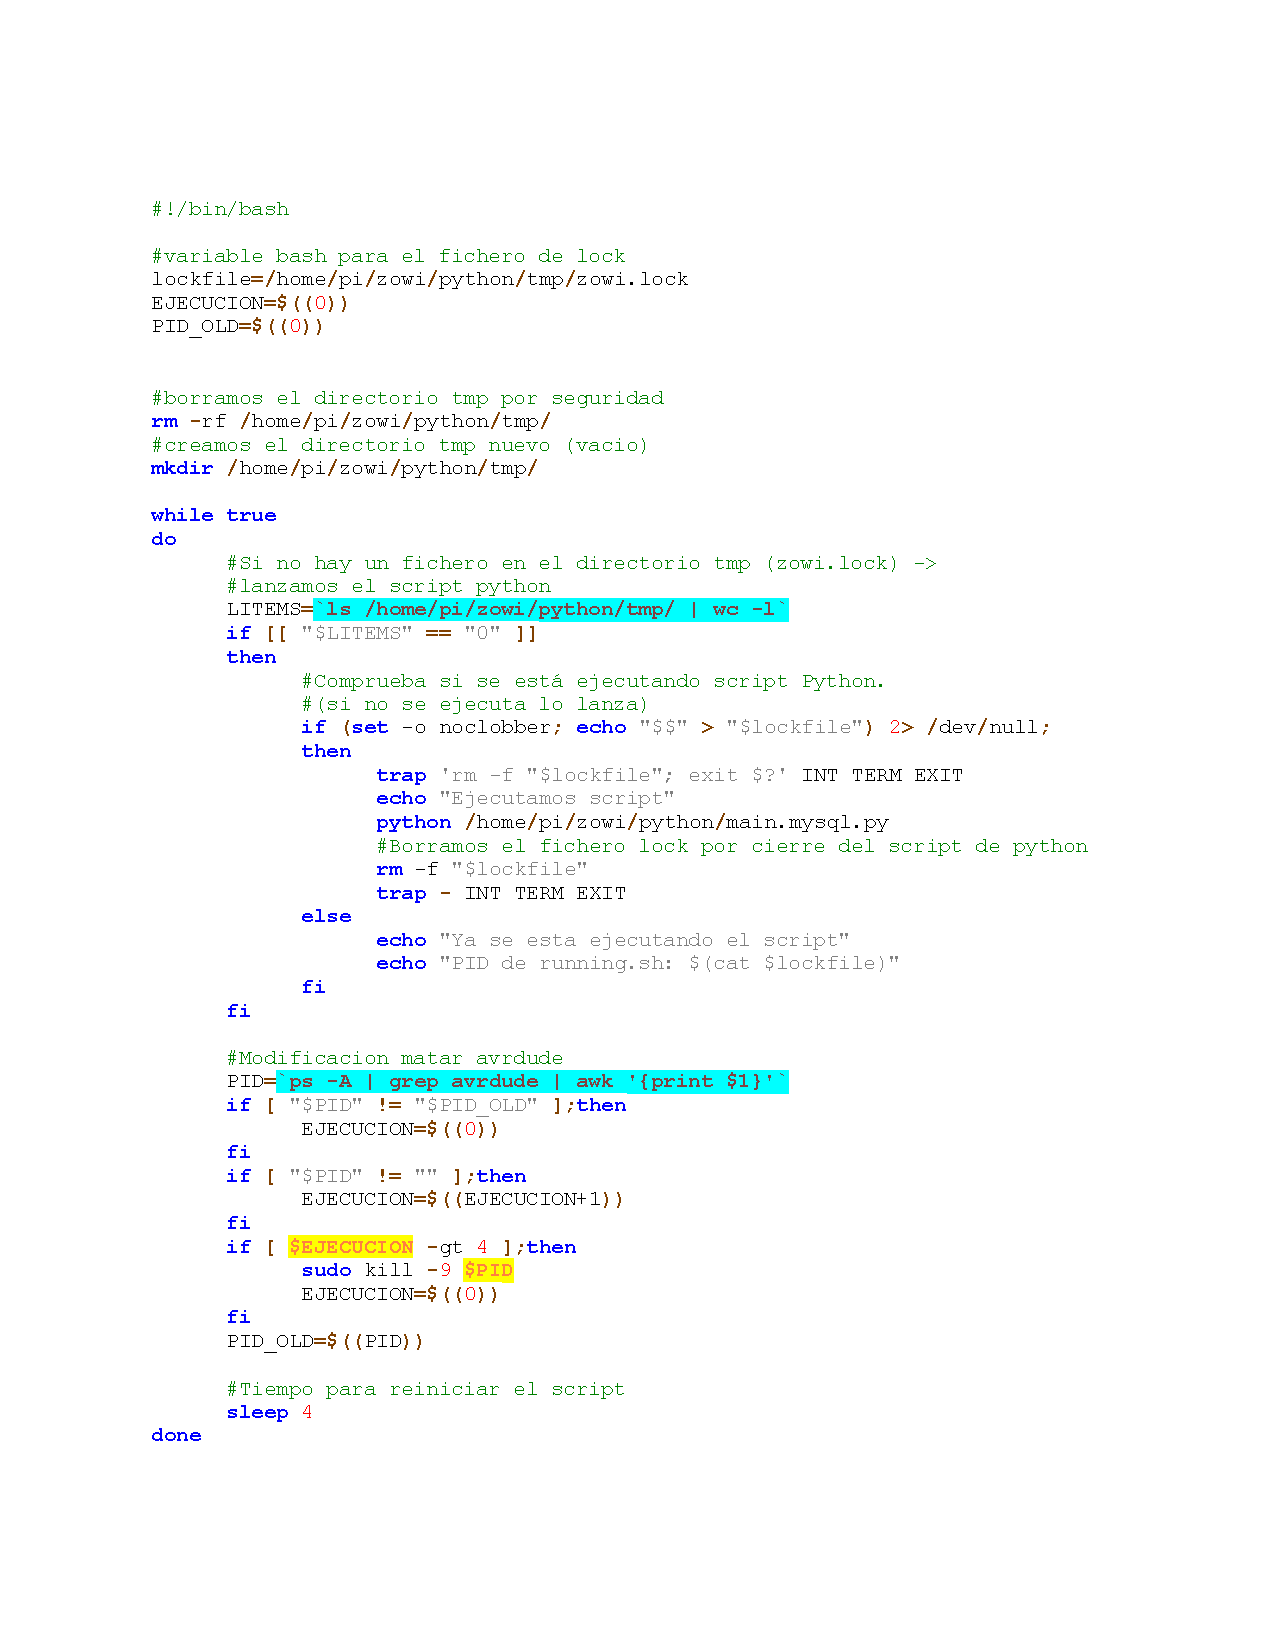
\includepdf[pages=-, pagecommand={}]{Appendices/externos/running.pdf}


\chapter{Fichero ZowiInit} % Main appendix title

\label{app:zowiinit} % For referencing this appendix elsewhere, use \ref{AppendixA}

ZowiInit lanzará la script running.sh al arranque del sistema. Se muestran también las instrucciones para hacerlo funcionar una vez creado y alojado en \textit{/etc/init.d/}.

\newpage

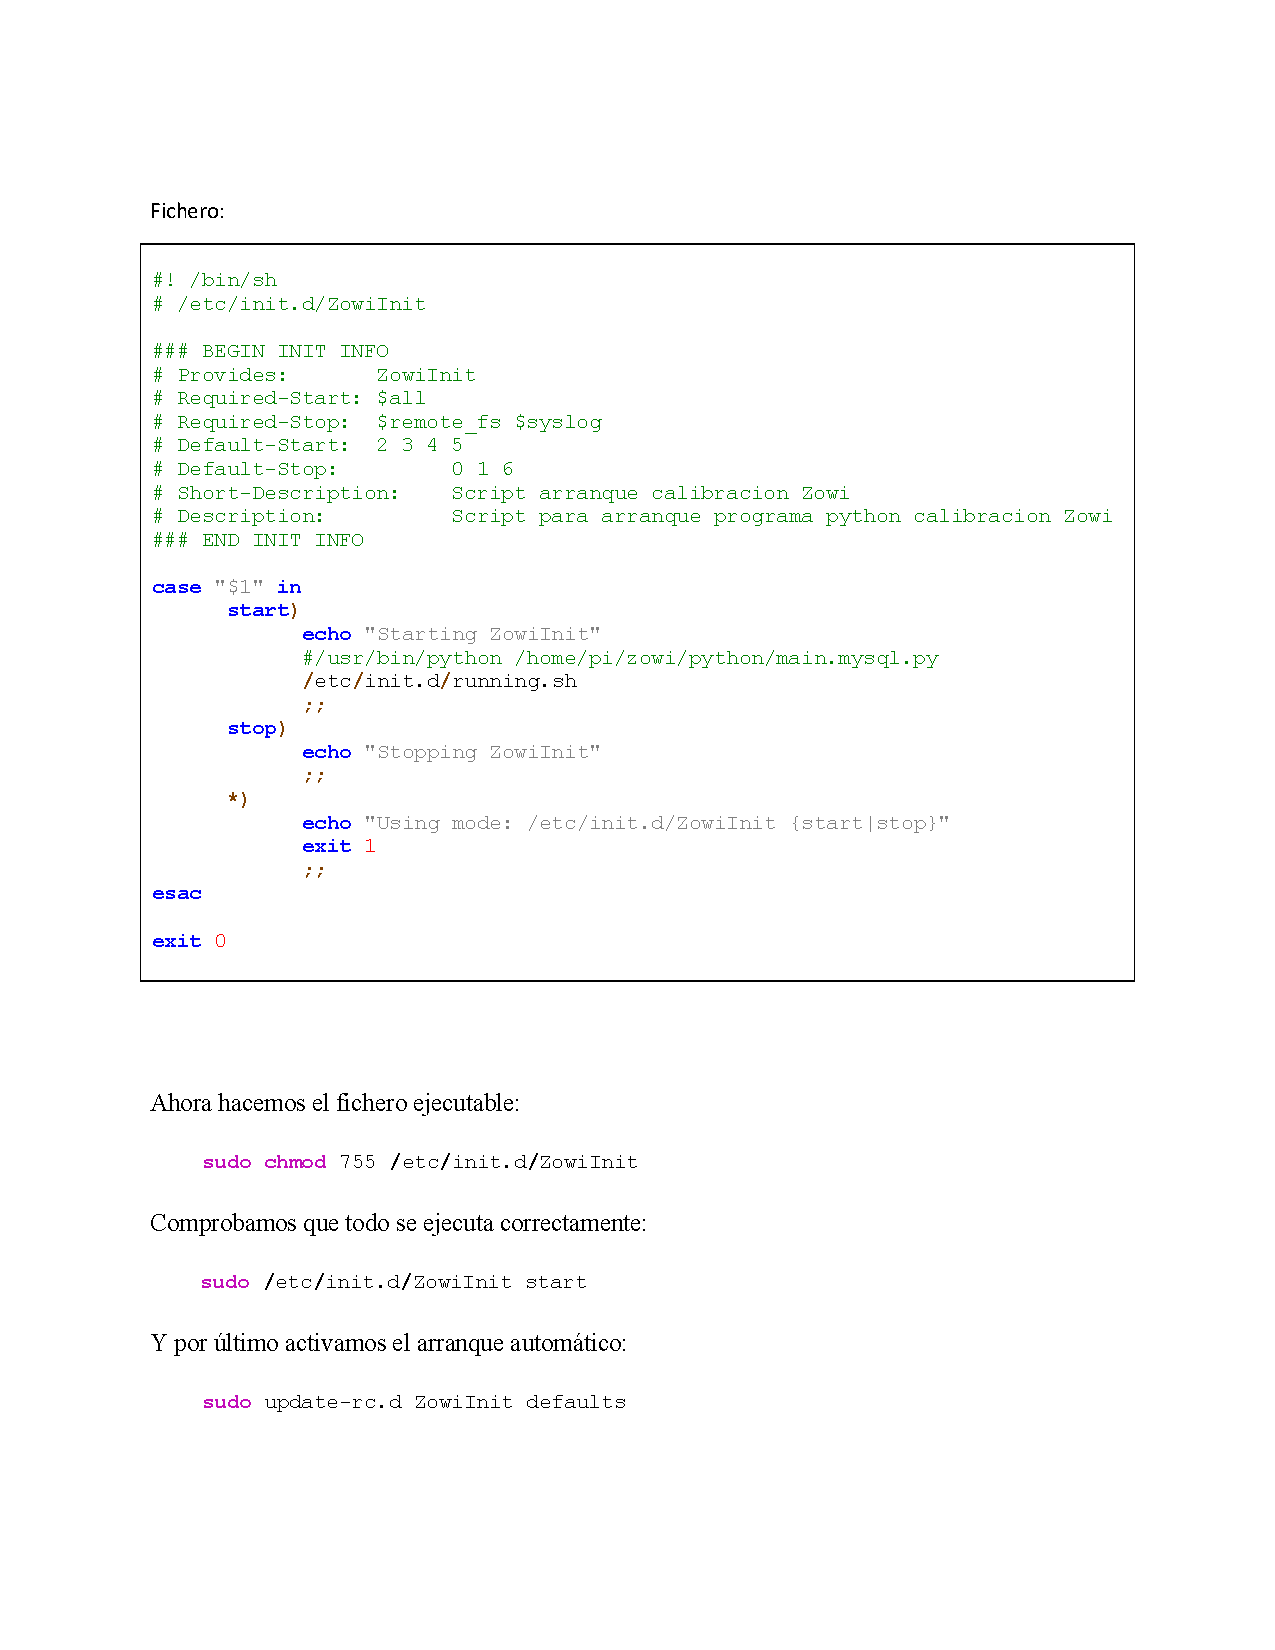
\includepdf[pages=-, pagecommand={}]{Appendices/externos/zowiinit.pdf}


\chapter{Autologin al inicio} % Main appendix title

\label{app:autologin} % For referencing this appendix elsewhere, use \ref{AppendixA}

Logeo de usuario automático al iniciar el sistema, sin pedir usuario ni contraseña.

\newpage

\includepdf[pages=-, pagecommand={}]{Appendices/externos/autologin.pdf}


\chapter{Reglas puertos USB} % Main appendix title

\label{app:rules} % For referencing this appendix elsewhere, use \ref{AppendixA}

Instrucciones del fichero rules para asignar alias a los puertos USB.

\newpage

\includepdf[pages=-, pagecommand={}]{Appendices/externos/rules.pdf}


\chapter{Notas de instalación Raspberry} % Main appendix title

\label{app:raspi-tips} % For referencing this appendix elsewhere, use \ref{AppendixA}

Documento de anotaciones sobre la configuración realizada en Raspberry.

\newpage

\includepdf[pages=-, pagecommand={}]{Appendices/externos/raspi-tips.pdf}


\chapter{Código Raspberry} % Main appendix title

\label{app:pythoncode} % For referencing this appendix elsewhere, use \ref{AppendixA}

Programa principal de la Raspberry, escrito en python: Fichero con nombre \textbf{main.mysql.py}.

\newpage

\includepdf[pages=-, pagecommand={}]{Appendices/externos/pythoncode.pdf}


\chapter{Código Mega} % Main appendix title

\label{app:megacode} % For referencing this appendix elsewhere, use \ref{AppendixA}

Programa principal de la Mega, de Arduino: Se muestra el programa principal para uno de los armarios ligeramente retocado (indents y saltos de línea principalmente). Las diferencias entre distintos armarios serán solamente los valores de calibración del acelerómetro.

\newpage

\includepdf[pages=-, pagecommand={}]{Appendices/externos/megacode.pdf}


\chapter{Código Zowi} % Main appendix title

\label{app:zowicode} % For referencing this appendix elsewhere, use \ref{AppendixA}

Programa intérprete que se descarga en Zowi para ser calibrado.

\newpage

\includepdf[pages=-, pagecommand={}]{Appendices/externos/zowicode.pdf}


\chapter{Especificaciones Mega} % Main appendix title

\label{app:mega-specs} % For referencing this appendix elsewhere, use \ref{AppendixA}

Especificaciones de la Freaduino Mega 2560: se muestran las especificaciones de la original Arduino Mega 2560 en primer lugar y los cambios de la versión clónica.

\newpage

\includepdf[pages=-, pagecommand={}]{Appendices/externos/mega-specs.pdf}


\chapter{Especificaciones Raspberry} % Main appendix title

\label{app:raspi-specs} % For referencing this appendix elsewhere, use \ref{AppendixA}

Especificaciones de la Raspberry PI 2 Model B.

\newpage

\includepdf[pages=-, pagecommand={}]{Appendices/externos/raspi-specs.pdf}



%----------------------------------------------------------------------------------------
%	BIBLIOGRAPHY
%----------------------------------------------------------------------------------------

\printbibliography[heading=bibintoc]

%----------------------------------------------------------------------------------------

\end{document}
